% -*- TeX-PDF-mode: t -*-

% XXX 12pt?  Measure is a bit long in 11pt.  Note: If I change the
% document font size, be sure to match the x-height of \code.
% XXX Use monospace for \code?

% draft - Fast compilation, all XXX notes, draft+git footers
%\documentclass[11pt,twoside,draft]{mitthesis}
% (no option) - Full compilation, all XXX notes, draft+git footer
\documentclass[11pt,twoside]{mitthesis}
% final - Full compilation, no XXX notes, no footer
%\documentclass[11pt,twoside,final]{mitthesis}

\usepackage[square,comma,numbers,sort&compress]{natbib}

% Put hyperref in final mode; otherwise hyperlinks are disabled
\usepackage[pdfauthor={Austin T. Clements},
            pdftitle={The Scalable Commutativity Rule: Designing Scalable Software for Multicore Processors},
            breaklinks,hidelinks,final]{hyperref}

% Fonts
\usepackage[T1]{fontenc}
\usepackage{amssymb}
\usepackage[defaultsans]{lato}
% [lf] - Use lining figures by default.  Mostly because I say things
% like "CPU 0" a lot in the text and old style figures make that look
% really weird.
\usepackage[lf,footnotefigures]{MinionPro} % After amssymb
\usepackage[toc,bib]{tabfigures}
% No Minion Pro?  Uncomment the next line to use Times
%\usepackage{times,mathptmx}
\usepackage{mathrsfs}

\usepackage{textcomp}
\usepackage{verbatim}
\usepackage{amsmath}
\usepackage{amsfonts}
\usepackage{xspace}
\usepackage{xcolor}
\usepackage{graphicx}
\usepackage{url}
\usepackage{listings}
\usepackage{balance}
\usepackage{gnuplot-lua-tikz}
\usepackage{subfig}
\usepackage{booktabs}
\usepackage{multirow}
\usepackage{rotating}
\usepackage{fancyvrb}
\usepackage{lastpage}
\usepackage{alltt}
\usepackage{etoolbox}
\usepackage{ifdraft}
\usepackage{titlesec}
\usepackage{cleveref} % After hyperref, listings
\IfFileExists{microtype.sty}{
  \usepackage{microtype}
}{
  \PackageError{microtype}{Package microtype not found.  Please
    install texlive-latex-recommended}{}
}

% Local packages below here

\usepackage{xxxnotes}
\usepackage{gitinfo}
\usepackage{wordnum}

\usepackage{scp-macros}
\usetikzlibrary{calc}
\usetikzlibrary{shapes.geometric}
\usetikzlibrary{shapes.misc}

\input{glyphtounicode}
\pdfgentounicode=1

\DeclareMathAlphabet{\mathcal}{OMS}{cmsy}{m}{n}

% If we're building without Minion Pro, define away \figureversion and
% \sscshape
\ifx\figureversion\undefined%
  \def\figureversion#1{}
\fi
\ifx\sscshape\undefined%
  \let\sscshape=\scshape
\fi

% Draft footer
\ifoptiondraft{\fancyfoot[L]{\textbf{FAST DRAFT}}}%
{\ifoptionfinal{}{\fancyfoot[L]{\textbf{DRAFT}}}}%

% Set page number footer in old style numerals
\fancyfoot[C]{{\figureversion{text}\thepage}}

% One space after periods
\frenchspacing

% Avoid widows and orphans
\widowpenalty=500
\clubpenalty=500

% Double spacing is too big; single spacing is too small
\linespread{1.15}

% Disable annoying inter-paragraph vertical spacing
\raggedbottom

% Aggressive figure placement
\renewcommand{\topfraction}{0.9}
\renewcommand{\bottomfraction}{0.8}
\setcounter{topnumber}{2}
\setcounter{bottomnumber}{2}
\setcounter{totalnumber}{4}
\setcounter{dbltopnumber}{2}
\renewcommand{\dbltopfraction}{0.9}
\renewcommand{\textfraction}{0.07}
\renewcommand{\floatpagefraction}{0.7}
\renewcommand{\dblfloatpagefraction}{0.7}

\setlength{\marginparwidth}{0.8in}

% For text from the SOSP paper, define CompactItemize
\newenvironment{CompactItemize}{\begin{itemize}}{\end{itemize}}

% Fix things like \emph{foo\xspace}.  See
% http://tug.org/pipermail/texhax/2006-November/007339.html
\makeatletter
\xspaceaddexceptions{\check@icr}
\makeatother

% Listing style
\lstset{basicstyle=\fontsize{9}{9}\sffamily,showstringspaces=false,columns=fullflexible}

% Use \code{...} for inline code.  Note that \code will typeset
% hyphens as minus signs.  You can use $math$ in \code.
\makeatletter
\def\@mathcode#1{\text{\code{#1}}}
\def\@regcode{\lstinline[mathescape=true]}
\def\@code{\ifmmode\let\next\@mathcode\else\let\next\@regcode\fi\next}
\def\code{\protect\@code}
\makeatother
\let\syscall=\code
% Code in gnuplot labels
\def\gpcode#1{{\fontsize{9}{9}\sffamily #1}}
% Command names.  The literate= hack makes listings use a regular
% hyphen instead of a minus sign, which is important for \cmd and
% happens to never matter for \code.
%\newcommand{\cmd}[1]{{\lstset{literate={-}{{-}}1}\code{#1}}}
% The above stopped working, but we don't do anything complex where we
% use \cmd, so use a simple definition.
\newcommand{\cmd}[1]{{\fontsize{9}{9}\sffamily #1}}
\let\gpcmd=\gpcode
% Don't set command names differently
%\newcommand{\cmd}[1]{#1}
%\newcommand{\gpcmd}[1]{#1}

\RecustomVerbatimEnvironment{Verbatim}{Verbatim}{formatcom=\footnotesize}

\renewcommand{\ttdefault}{pxtt}

\newcommand{\vm}{RadixVM\xspace}
\newcommand{\refcache}{Refcache\xspace}
\newcommand{\sys}{sv6\xspace}
\newcommand{\tool}{{\scshape Commuter}\xspace}
\newcommand{\analyzer}{{\scshape Analyzer}\xspace}
\newcommand{\testgen}{{\scshape Testgen}\xspace}
\newcommand{\mtrace}{{\scshape Mtrace}\xspace}
\newcommand{\SIM}{SIM\xspace}
\newcommand{\fs}{ScaleFS\xspace}

\newcommand{\inputcode}[1]{%
  {\small\hrule\vspace{0.5em}\input{#1}\hrule\vspace{0.5em}}}

\newcommand{\inputnodraft}[1]{%
  \ifdraft{#1 omitted in draft mode}{\input{#1}}}

\makeatletter
% XXX I'd much rather strip all periods from *all* captions in the
% list of figures, but I can't for the life of me get TeX to do that.
\def\sc@oneperiod#1.{\@ifnextchar.{\sc@oneperiod #1}{#1.}}
\newcommand{\splitcaption}[2]{%
  \caption[\protect\sc@oneperiod #1.]{#1 #2}}
\makeatother

\newcommand{\tikzshowbbox}{
  \path[draw=black] (current bounding box.north west)
    rectangle (current bounding box.south east);
  \fill[overlay,black] (0,0) circle (.5mm);
  \draw[overlay,black] (0,2mm) -- +(0,5mm) (0,-2mm) -- +(0,-5mm)
                       (2mm,0) -- +(5mm,0) (-2mm,0) -- +(-5mm,0);}

\bibpunct[: ]{[}{]}{,}{n}{XXX}{XXX}

% Do always capitalize "Figure".  Also override the default "Fig."
\crefname{figure}{Figure}{Figures}
\crefname{mysubfigure}{Figure}{Figures}
\Crefname{mysubfigure}{Figure}{Figures}
\newcommand{\thiscref}[1]{this \lcnamecref{#1}}
\newcommand{\Thiscref}[1]{This \lcnamecref{#1}}

% Single-line format with chapter number and a vertical bar.
% \titleformat{\chapter}[hang]{%
%   \huge\bfseries}{\thechapter\hspace{15pt}\rule[-1.2em]{.5pt}{3em}\hspace{15pt}}{0pt}{\huge\bfseries}

% Two-line format with spelled-out chapter number and a horizontal bar
% under the title.
\titleformat{\chapter}[display]%
  {\relax}%
  {\sscshape\Wordnum{\thechapter}}{1em}%
  {\huge\bfseries}[\titlerule]

% Make tables use the same numbering and format as figures
\makeatletter
\let\thetable\thefigure
\let\c@table\c@figure
\makeatother

% Fold the one table in to the list of figures
\makeatletter
\renewcommand\ext@table{lof}
\makeatother
\renewcommand\listfigurename{Figures and Tables}

\begin{document}

\input{pyexpr}

\makeatletter
\def\PY@reset{\let\PY@it=\relax \let\PY@bf=\relax%
    \let\PY@ul=\relax \let\PY@tc=\relax%
    \let\PY@bc=\relax \let\PY@ff=\relax}
\def\PY@tok#1{\csname PY@tok@#1\endcsname}
\def\PY@toks#1+{\ifx\relax#1\empty\else%
    \PY@tok{#1}\expandafter\PY@toks\fi}
\def\PY@do#1{\PY@bc{\PY@tc{\PY@ul{%
    \PY@it{\PY@bf{\PY@ff{#1}}}}}}}
\def\PY#1#2{\PY@reset\PY@toks#1+\relax+\PY@do{#2}}

\expandafter\def\csname PY@tok@gd\endcsname{\def\PY@tc##1{\textcolor[rgb]{0.63,0.00,0.00}{##1}}}
\expandafter\def\csname PY@tok@gu\endcsname{\let\PY@bf=\textbf\def\PY@tc##1{\textcolor[rgb]{0.50,0.00,0.50}{##1}}}
\expandafter\def\csname PY@tok@gt\endcsname{\def\PY@tc##1{\textcolor[rgb]{0.00,0.27,0.87}{##1}}}
\expandafter\def\csname PY@tok@gs\endcsname{\let\PY@bf=\textbf}
\expandafter\def\csname PY@tok@gr\endcsname{\def\PY@tc##1{\textcolor[rgb]{1.00,0.00,0.00}{##1}}}
\expandafter\def\csname PY@tok@cm\endcsname{\let\PY@it=\textit\def\PY@tc##1{\textcolor[rgb]{0.25,0.50,0.50}{##1}}}
\expandafter\def\csname PY@tok@vg\endcsname{\def\PY@tc##1{\textcolor[rgb]{0.10,0.09,0.49}{##1}}}
\expandafter\def\csname PY@tok@mh\endcsname{\def\PY@tc##1{\textcolor[rgb]{0.40,0.40,0.40}{##1}}}
\expandafter\def\csname PY@tok@go\endcsname{\def\PY@tc##1{\textcolor[rgb]{0.53,0.53,0.53}{##1}}}
\expandafter\def\csname PY@tok@ge\endcsname{\let\PY@it=\textit}
\expandafter\def\csname PY@tok@vc\endcsname{\def\PY@tc##1{\textcolor[rgb]{0.10,0.09,0.49}{##1}}}
\expandafter\def\csname PY@tok@il\endcsname{\def\PY@tc##1{\textcolor[rgb]{0.40,0.40,0.40}{##1}}}
\expandafter\def\csname PY@tok@cs\endcsname{\let\PY@it=\textit\def\PY@tc##1{\textcolor[rgb]{0.25,0.50,0.50}{##1}}}
\expandafter\def\csname PY@tok@cp\endcsname{\def\PY@tc##1{\textcolor[rgb]{0.74,0.48,0.00}{##1}}}
\expandafter\def\csname PY@tok@gi\endcsname{\def\PY@tc##1{\textcolor[rgb]{0.00,0.63,0.00}{##1}}}
\expandafter\def\csname PY@tok@gh\endcsname{\let\PY@bf=\textbf\def\PY@tc##1{\textcolor[rgb]{0.00,0.00,0.50}{##1}}}
\expandafter\def\csname PY@tok@ni\endcsname{\let\PY@bf=\textbf\def\PY@tc##1{\textcolor[rgb]{0.60,0.60,0.60}{##1}}}
\expandafter\def\csname PY@tok@nl\endcsname{\def\PY@tc##1{\textcolor[rgb]{0.63,0.63,0.00}{##1}}}
\expandafter\def\csname PY@tok@nn\endcsname{\let\PY@bf=\textbf\def\PY@tc##1{\textcolor[rgb]{0.00,0.00,1.00}{##1}}}
\expandafter\def\csname PY@tok@no\endcsname{\def\PY@tc##1{\textcolor[rgb]{0.53,0.00,0.00}{##1}}}
\expandafter\def\csname PY@tok@na\endcsname{\def\PY@tc##1{\textcolor[rgb]{0.49,0.56,0.16}{##1}}}
\expandafter\def\csname PY@tok@nb\endcsname{\def\PY@tc##1{\textcolor[rgb]{0.00,0.50,0.00}{##1}}}
\expandafter\def\csname PY@tok@nc\endcsname{\let\PY@bf=\textbf\def\PY@tc##1{\textcolor[rgb]{0.00,0.00,1.00}{##1}}}
\expandafter\def\csname PY@tok@nd\endcsname{\def\PY@tc##1{\textcolor[rgb]{0.67,0.13,1.00}{##1}}}
\expandafter\def\csname PY@tok@ne\endcsname{\let\PY@bf=\textbf\def\PY@tc##1{\textcolor[rgb]{0.82,0.25,0.23}{##1}}}
\expandafter\def\csname PY@tok@nf\endcsname{\def\PY@tc##1{\textcolor[rgb]{0.00,0.00,1.00}{##1}}}
\expandafter\def\csname PY@tok@si\endcsname{\let\PY@bf=\textbf\def\PY@tc##1{\textcolor[rgb]{0.73,0.40,0.53}{##1}}}
\expandafter\def\csname PY@tok@s2\endcsname{\def\PY@tc##1{\textcolor[rgb]{0.73,0.13,0.13}{##1}}}
\expandafter\def\csname PY@tok@vi\endcsname{\def\PY@tc##1{\textcolor[rgb]{0.10,0.09,0.49}{##1}}}
\expandafter\def\csname PY@tok@nt\endcsname{\let\PY@bf=\textbf\def\PY@tc##1{\textcolor[rgb]{0.00,0.50,0.00}{##1}}}
\expandafter\def\csname PY@tok@nv\endcsname{\def\PY@tc##1{\textcolor[rgb]{0.10,0.09,0.49}{##1}}}
\expandafter\def\csname PY@tok@s1\endcsname{\def\PY@tc##1{\textcolor[rgb]{0.73,0.13,0.13}{##1}}}
\expandafter\def\csname PY@tok@sh\endcsname{\def\PY@tc##1{\textcolor[rgb]{0.73,0.13,0.13}{##1}}}
\expandafter\def\csname PY@tok@sc\endcsname{\def\PY@tc##1{\textcolor[rgb]{0.73,0.13,0.13}{##1}}}
\expandafter\def\csname PY@tok@sx\endcsname{\def\PY@tc##1{\textcolor[rgb]{0.00,0.50,0.00}{##1}}}
\expandafter\def\csname PY@tok@bp\endcsname{\def\PY@tc##1{\textcolor[rgb]{0.00,0.50,0.00}{##1}}}
\expandafter\def\csname PY@tok@c1\endcsname{\let\PY@it=\textit\def\PY@tc##1{\textcolor[rgb]{0.25,0.50,0.50}{##1}}}
\expandafter\def\csname PY@tok@kc\endcsname{\let\PY@bf=\textbf\def\PY@tc##1{\textcolor[rgb]{0.00,0.50,0.00}{##1}}}
\expandafter\def\csname PY@tok@c\endcsname{\let\PY@it=\textit\def\PY@tc##1{\textcolor[rgb]{0.25,0.50,0.50}{##1}}}
\expandafter\def\csname PY@tok@mf\endcsname{\def\PY@tc##1{\textcolor[rgb]{0.40,0.40,0.40}{##1}}}
\expandafter\def\csname PY@tok@err\endcsname{\def\PY@bc##1{\setlength{\fboxsep}{0pt}\fcolorbox[rgb]{1.00,0.00,0.00}{1,1,1}{\strut ##1}}}
\expandafter\def\csname PY@tok@kd\endcsname{\let\PY@bf=\textbf\def\PY@tc##1{\textcolor[rgb]{0.00,0.50,0.00}{##1}}}
\expandafter\def\csname PY@tok@ss\endcsname{\def\PY@tc##1{\textcolor[rgb]{0.10,0.09,0.49}{##1}}}
\expandafter\def\csname PY@tok@sr\endcsname{\def\PY@tc##1{\textcolor[rgb]{0.73,0.40,0.53}{##1}}}
\expandafter\def\csname PY@tok@kn\endcsname{\let\PY@bf=\textbf\def\PY@tc##1{\textcolor[rgb]{0.00,0.50,0.00}{##1}}}
\expandafter\def\csname PY@tok@gp\endcsname{\let\PY@bf=\textbf\def\PY@tc##1{\textcolor[rgb]{0.00,0.00,0.50}{##1}}}
\expandafter\def\csname PY@tok@kr\endcsname{\let\PY@bf=\textbf\def\PY@tc##1{\textcolor[rgb]{0.00,0.50,0.00}{##1}}}
\expandafter\def\csname PY@tok@s\endcsname{\def\PY@tc##1{\textcolor[rgb]{0.73,0.13,0.13}{##1}}}
\expandafter\def\csname PY@tok@kp\endcsname{\def\PY@tc##1{\textcolor[rgb]{0.00,0.50,0.00}{##1}}}
\expandafter\def\csname PY@tok@w\endcsname{\def\PY@tc##1{\textcolor[rgb]{0.73,0.73,0.73}{##1}}}
\expandafter\def\csname PY@tok@ow\endcsname{\let\PY@bf=\textbf\def\PY@tc##1{\textcolor[rgb]{0.67,0.13,1.00}{##1}}}
\expandafter\def\csname PY@tok@sb\endcsname{\def\PY@tc##1{\textcolor[rgb]{0.73,0.13,0.13}{##1}}}
\expandafter\def\csname PY@tok@k\endcsname{\let\PY@bf=\textbf\def\PY@tc##1{\textcolor[rgb]{0.00,0.50,0.00}{##1}}}
\expandafter\def\csname PY@tok@se\endcsname{\let\PY@bf=\textbf\def\PY@tc##1{\textcolor[rgb]{0.73,0.40,0.13}{##1}}}
\expandafter\def\csname PY@tok@sd\endcsname{\let\PY@it=\textit\def\PY@tc##1{\textcolor[rgb]{0.73,0.13,0.13}{##1}}}

\def\PYZbs{\char`\\}
\def\PYZus{\char`\_}
\def\PYZob{\char`\{}
\def\PYZcb{\char`\}}
\def\PYZca{\char`\^}
\def\PYZam{\char`\&}
\def\PYZlt{\char`\<}
\def\PYZgt{\char`\>}
\def\PYZsh{\char`\#}
\def\PYZpc{\char`\%}
\def\PYZdl{\char`\$}
\def\PYZhy{\char`\-}
\def\PYZsq{\char`\'}
\def\PYZdq{\char`\"}
\def\PYZti{\char`\~}
% for compatibility with earlier versions
\def\PYZat{@}
\def\PYZlb{[}
\def\PYZrb{]}
\makeatother



% -*- TeX-master: "paper.tex"; TeX-PDF-mode: t -*-

\title{The Scalable Commutativity Rule: \\ Designing Scalable Software for
  Multicore Processors}
\author{Austin T. Clements}
\prevdegrees{
  S.B., Massachusetts Institute of Technology (2006) \\
  M.Eng., Massachusetts Institute of Technology (2008)}
\department{Department of Electrical Engineering and Computer Science}
\degree{Doctor of Philosophy in Computer Science}
\degreemonth{June}
\degreeyear{2014}
\thesisdate{\XXX!{date}}
\supervisor{M. Frans Kaashoek}{Professor \XXX{full title?}}
\chairman{Leslie A. Kolodziejski}{Chair, Department Committee
  on Graduate Theses}
\maketitle

\cleardoublepage

\begin{abstractpage}
% $Log: abstract.tex,v $
% Revision 1.1  93/05/14  14:56:25  starflt
% Initial revision
% 
% Revision 1.1  90/05/04  10:41:01  lwvanels
% Initial revision
% 
%
%% The text of your abstract and nothing else (other than comments) goes here.
%% It will be single-spaced and the rest of the text that is supposed to go on
%% the abstract page will be generated by the abstractpage environment.  This
%% file should be \input (not \include 'd) from cover.tex.
In this thesis, I designed and implemented a compiler which performs
optimizations that reduce the number of low-level floating point operations
necessary for a specific task; this involves the optimization of chains of
floating point operations as well as the implementation of a ``fixed'' point
data type that allows some floating point operations to simulated with integer
arithmetic.  The source language of the compiler is a subset of C, and the
destination language is assembly language for a micro-floating point CPU.  An
instruction-level simulator of the CPU was written to allow testing of the
code.  A series of test pieces of codes was compiled, both with and without
optimization, to determine how effective these optimizations were.

\end{abstractpage}
\cleardoublepage

\begin{singlespace}
\chapter*{Acknowledgments}

\XXX![AC]{Update}

We thank Silas Boyd-Wickizer, Marc Shapiro, Rachid Guerraoui,
Butler Lampson, the anonymous reviewers, and our
shepherd, Jon Howell, for their feedback.
%
Additionally, Silas Boyd-Wickizer contributed to much of the
implementation of \sys.
%
This research was supported by NSF awards SHF-964106 and CNS-1301934,
by Quanta, and by Google. Eddie Kohler was partially supported by a
Microsoft Research New Faculty Fellowship and a Sloan Research
Fellowship.



This dissertation incorporates and extends work previously published
in the following papers:

\begin{quote}
  Austin~T. Clements, M.~Frans Kaashoek, Nickolai Zeldovich,
  Robert~T. Morris, and Eddie Kohler.
  \newblock The scalable commutativity rule: Designing scalable
  software for multicore processors.
  \newblock In \emph{Proceedings of the 24th ACM Symposium on
    Operating Systems Principles (\mbox{SOSP})}, Farmington,
  Pennsylvania, November 2013.

  Austin~T. Clements, M.~Frans Kaashoek, and Nickolai Zeldovich.
  \newblock {RadixVM}: Scalable address spaces for multithreaded
  applications.
  \newblock In \emph{Proceedings of the ACM EuroSys Conference},
  Prague, Czech Republic, April 2013.

  Austin~T. Clements, M.~Frans Kaashoek, and Nickolai Zeldovich.
  \newblock Concurrent address spaces using {RCU} balanced trees.
  \newblock In \emph{Proceedings of the 17th International Conference
    on Architectural Support for Programming Languages and Operating
    Systems (\mbox{ASPLOS})}, London, UK, March 2012.
\end{quote}

\end{singlespace}

\pagestyle{plain}
\tableofcontents
\newpage
\listoffigures
\XXX!{Check for overlong captions and use splitcaption}

% The preamble folded tables in to the list of figures
% \newpage
% \listoftables

% Shift sectioning commands to start at \chapter
\let\subsubsubsection\subsubsection
\let\subsubsection\subsection
\let\subsection\section
\let\section\chapter

\section{Introduction}
\label{sec:intro}

\XXX[STATUS]{Re-organized and expanded from SOSP.  Draft almost
  ready.}

This dissertation presents a pragmatic and formal approach to the
design and implementation of scalable multicore software that spans
from the earliest stages of software interface conception through
testing and maintenance of complete implementations.

The rest of \thiscref{sec:intro} introduces the multicore
architectures that have taken over general-purpose computing, the
problematic ways in which software developers are coping with these
new architectures, and our solution to the design and implementation
of software for multicore architectures.


%\subsection{The rise of multicore architectures}
\subsection{Parallelize or perish}

Until the mid-2000's, writing higher performance software got easier
with every passing year as each new CPU model clambered for higher
clock speeds and greater computational throughput.
%
But higher clock speeds require more power and generate more heat, and
around 2005 clock speeds brought CPUs to the thermal dissipation
limits of a few square centimeters of silicon.
%
CPU architects could no longer significantly increase clock speeds, so
instead they began increasing parallelism, putting more cores on the
same chip, providing more and more independent processing units, while
maintaining shared access to memory and I/O resources.
% maintaining a ``coherent'' view of memory and shared access to I/O
% resources.
%
% With the rise of multicore architectures, parallel programming went
% from niche to necessary.
With the widespread adoption of multicore architectures for
general-purpose computing, parallel programming went from niche to
necessary.
%
All software must now be parallel to perform.
%
But, while software performance naturally scales with clock speed,
scaling with parallelism is an untamed problem.  Even with careful
engineering, software rarely achieves the holy grail of \emph{linear
  scalability}, where doubling the hardware parallelism doubles the
software's performance.

Operating system kernels are a poignant example of both the importance
of parallelism and the difficulty of achieving it.
%
As the common substrate that provides shared services and resources
that most applications depend heavily on, any limits on kernel
scalability become limits on application scalability.
%
Kernels must deal with interactions within and between applications
and cope with diverse and unknown workloads.
%
% \XXX{example?  Any application that creates, opens, read, or writes
%   files is at risk of contending with any other application that uses
%   the file system if the kernel's implementation is insufficiently
%   parallel.}
%
Underlining the importance of kernel scalability, Linux kernel
developers have put vast amounts of effort into multicore Linux,
bringing it to the forefront of putting parallel programming
techniques into practice.  Lock-free data structures, read-copy-update
garbage collection, per-core data, and sophisticated synchronization
mechanisms are all commonplace in the Linux kernel.

Yet, despite the extensive efforts of kernel and application
developers alike, scaling software performance on multicores remains
an inexact science dominated by guesswork, measurement, and expensive
cycles of redesign.
%
The state of the art for evaluating and improving the scalability of
multicore software is the choose some workload, plot performance at
varying numbers of cores, and use tools such as differential
profiling~\cite{mckenney:differential} to identify scalability
bottlenecks.  \XXX[AC]{Should we cite anything for this?  Is there
  anything to cite besides our own papers?}  \XXX[AC]{Mention that
  this is an evolution of sequential optimization techniques?}
%
This focuses developer effort on demonstrable issues, but is
ultimately a near-sighted approach.
%
% Different workloads and higher core counts often reveal new
% bottlenecks, leading to a Sisyphean cycle of performance catch-up and
% leaving workloads and hardware that kernel developers don't have
% access to to fend for themselves.
%
Each new hardware model and workload powers a Sisyphean cycle of
finding and fixing new bottlenecks.
%
Projects such as Linux require continuous infusions of manpower to
maintain their scalability edge and even then, workloads and hardware
that kernel developers don't have access to are a scalability gamble.
%
But the deeper problem with this workload-driven approach is that many
scalability problems lie not in the implementation, but in the
software interface.  By the time developers have an implementation, a
workload, and the hardware to demonstrate a bottleneck,
interface-level solutions may be impractical or impossible.

Consider the POSIX~\cite{posix2013} \code{open} call, which opens a
file by name and returns a \emph{file descriptor}, a number used to
identify the open file in later operations.
%
Even though this identifier is opaque, POSIX requires that \code{open}
return the numerically lowest available file descriptor for the
calling process, forcing the kernel to serialize file descriptor
allocation between threads in a process.
%
This simplified the kernel interface during the early days of Unix,
but this interface design choice is now a burden on implementation
scalability.
%
It's an unnecessary burden, too: a simple change to allow \code{open}
to return \emph{any} available file descriptor would enable the kernel
to choose file descriptors scalably.
%
This particular example is well-known~\cite{boyd-wickizer:corey}, but
myriad subtler issues exist in POSIX and other interfaces.

Interface design choices have implications for implementation
scalability.
%
If interface designers could distinguish interfaces that definitely
have a scalable implementation from those that don't, they would have
the predictive power to design \emph{scalable interfaces} that enable
scalable implementations.


\subsection{A rule for interface design}

This dissertation presents a new approach to scalability that starts
at scalable software interface design.
%
This makes reasoning about multicore scalability possible before an
implementation exists and before the necessary hardware is available
to measure the implementation's scalability.  It can highlight
inherent scalability problems, leading to alternate interface designs.
And it sets a clear scaling target for the implementation of a
scalable interface and enables systematic testing of an
implementation's scalability.

Scalability is often considered an implementation property, not an
interface property, not least because what scales depends on hardware.
%
However, modern shared-memory multicores use local caches and
protocols like MESI~\cite{papamarcos:mesi} to provide a globally
consistent ``coherent'' view of memory.  This general architecture
enables general arguments about scalability.
%
On such processors, a core can scalably read and write data it has
cached exclusively, and scalably read data it has cached in shared
mode. Writing a cache line that was last read or written by another
core is not scalable, however, since the coherence protocol serializes
ownership changes for each cache line, and because the shared
interconnect may serialize unrelated transfers.

We therefore say that a set of operations scales if their
implementations have \emph{conflict-free} memory accesses; that is, no
core writes a cache line that was read or written by another core.
%
When memory accesses are conflict-free, adding more cores will produce
a linear increase in capacity.
%
This is not a perfect model of the complex realities of modern
hardware, but it is a good approximation that we confirm in
\cref{sec:scalability}.

At the core of our approach is this \emph{scalable commutativity
  rule}: In any situation where several operations
\emph{commute}---meaning there's no way to distinguish their execution
order using the interface---they have an implementation whose memory
accesses are conflict-free during those operations.
%
Or, more concisely, \textbf{whenever interface operations commute,
  they can be implemented in a way that scales.}

This rule makes intuitive sense: when operations commute, their
results (return value and effect on system state) are independent of
order.  Hence, communication between commutative operations is
unnecessary, and eliminating it yields conflict-free and scalable
implementations.

The commutativity rule leads to a new way to design scalable
software:
%
analyze the interface's commutativity; if possible, refine or redesign
the interface to improve its commutativity, and then design an
implementation that scales in commutative situations.
%
For example,
consider file creation in a POSIX-like file system. Imagine that
multiple processes create files in the same directory at the same
time. Can the creation system calls be made to scale? Our
first answer was ``obviously not'': the system calls modify the same
directory, so surely the implementation must
serialize access to the directory. But it turns
out these operations commute if the two files have different names
(and no hard or symbolic links are involved) and, therefore, have an
implementation that scales for such names.
One such implementation represents each directory as a hash table
indexed by file name, with an independent lock per bucket,
so that creation of differently named files is conflict-free, barring
hash collisions.
%
Before the rule, we tried to determine if these
operations could scale by analyzing all of the \emph{implementations}
we could think
of.  This process was difficult, unguided, and itself did not scale to
complex interfaces, which
motivated our goal of reasoning about
scalability in terms of interfaces.


\subsection{Contributions}

\XXX{Should more of this stuff go into the rule section and this just
  be a summary?}

The rest of this dissertation presents the scalable commutativity rule
in depth and explores its consequences from interface design to
implementation to testing.

The intuition for the rule presented above is useful in practice, but
not precise enough to reason
about formally.
%
Therefore, the first contribution of this dissertation is a
formalization of the scalable commutativity rule and a proof of the
correctness of this formalized form, which we present in
\cref{sec:rule}.
%
Connecting this formalization to scalability as traditionally measured
requires certain assumptions about multicore hardware, which we verify
experimentally in \cref{sec:scalability}.

An important consequence of this presentation is a novel form of
commutativity we name \emph{\SIM\ commutativity}.
%
The usual definition of commutativity (e.g., for algebraic operations)
is so stringent that it rarely applies to the complex, stateful
interfaces common in systems software.
%
\SIM\ commutativity, in contrast, is \emph{state-dependent} and
\emph{interface-based}, as well as \emph{monotonic}.
%
When operations commute in the context of a specific system state,
specific operation arguments, and specific concurrent operations, we
show that an implementation exists that is conflict-free \emph{for that state
  and those arguments and concurrent operations}.
%
This exposes many more opportunities to apply the rule to real
interfaces---and thus discover scalable implementations---than a more
conventional notion of commutativity would.
%
Despite its logical state dependence, \SIM\ commutativity is
interface-based: rather than requiring all operation orders to produce
identical internal states, it requires the resulting states to be
indistinguishable via the interface.
%
\SIM\ commutativity is thus independent of any specific
implementation, enabling developers to apply the rule directly to
interface design.

Putting the rule into practice, in \cref{sec:posix} this dissertation
contributes a set of general guidelines for designing interfaces that
enable scalable implementations, inspired by both the successes and
failures of POSIX.  In these guidelines, we propose specific
modifications to POSIX that would allow for greater scalability.

However, complex interfaces are still complex, and even given the rule
and these interface design guidelines, it can be difficult to spot and
reason about all commutative cases.
%
% Complex interfaces can make it difficult to spot and reason about all
% commutative cases even given the rule.
%
To address this challenge, this dissertation introduces a method to
automate reasoning about interfaces and implementations, embodied in a
software tool named \tool, presented in \cref{sec:tool}.
%
\tool takes an interface model
in the form of a simplified, symbolic implementation, computes precise
conditions under which sets of operations commute, and tests an
implementation for conflict-freedom under these conditions.  This tool can be
integrated into the software development process to drive initial design and
implementation, to incrementally improve existing implementations, or to
help developers understand the commutativity of an interface.

In \cref{sec:topic:model}, we apply \tool to a simplified model of
\pyexpr{len(mscan.calls)} POSIX file system and virtual memory system
calls.
%
From this model,
\tool generates \pyexpr{mscan.ntestcases} tests of commutative
system call pairs, all of which can be made conflict-free
according to the rule.
%
Applying this suite to Linux, we find that the Linux kernel is
conflict-free for \pyexpr{mscan.ntestcases - mscan.linux.shared}
(\pyexpr{percent(1-(mscan.linux.shared/float(mscan.ntestcases)))}) of
these cases.
%
Many of the commutative cases where Linux is not conflict-free are
important to applications---such as commutative
\code{mmap}s and creating different files in a shared directory---and
reflect findings in previous work~\cite{boyd-wickizer:scaling}.

Finally, to demonstrate the application of the rule and \tool to the
design and implementation of a real system, we use these tests to
guide the implementation of a new research operating system kernel
named \sys.
%
\sys doubles as an existence proof showing that the rule can be
applied fruitfully to the design and implementation of a large
software system, and as an embodiment of novel scalable kernel
implementation techniques.
%
\Cref{sec:sv6} details these techniques and the software designs
necessary to achieve conflict-free commutative operations in \sys's
virtual memory system (\vm) and in-memory file system (\fs).
%
\tool verifies that \sys is conflict-free for
\pyexpr{mscan.ntestcases - mscan.xv6.shared}
(\pyexpr{percent(1-(mscan.xv6.shared/float(mscan.ntestcases)))})
of the tests generated by our POSIX model and addresses many of the
sources of conflicts found in the Linux kernel.
%
\Cref{sec:eval} confirms that \sys's conflict-free implementations of
commutative system calls translate to dramatic improvements in
scalability for both microbenchmarks and application benchmarks on an
80-core x86 machine.

% The paper is organized as follows.  \S\ref{sec:related} relates our thinking
% about scalability to previous work. \S\ref{sec:rule} introduces the
% commutativity rule and argues its correctness. \S\ref{sec:posix} applies the
% rule to an OS interface, identifying opportunities for
% commutativity. \S\ref{sec:tool} describes \tool{}.  \S\ref{sec:model} describes
% \fs and how \tool{} drove its implementation. \S\ref{sec:eval} shows that using
% the commutativity rule results in better scalability on real
% hardware. \S\ref{sec:concl} summarizes our conclusions.

% LocalWords:  rule's RCU microbenchmarks

% -*- fill-column: 80 -*-

\section{Related Work}
\label{sec:related}

The primary contribution of this work is the commutativity rule and its
use in the design and implementation of software systems.  This section
relates this contribution to previous work on scalability, operating
system design, and commutativity.

\subsection{Thinking about scalability}

Israeli and Rappoport introduce the notion of disjoint access parallelism.
In particular, they point out that concurrent programs that access
memory locations disjointly won't experience hotspots, and thus 
are scalable~\cite{israeli:disjoint-access}.  We build on a similar intuition.
A key advance proposed in this work is to reason about the potential
for scalability at the level of interfaces, as opposed to the
scalability of a given implementation or memory access trace.
In particular, we aim to connect the commutativity of interfaces to the
potential for disjoint access parallelism.

Both the original disjoint access parallelism paper and subsequent work,
including the paper by Roy et al.~\cite{roy:limits-dap}, explore
the scalability of applications that have some amount of non-disjoint
sharing, such as compare-and-swap instructions on a shared cache line
or a shared lock.  As part of this research, we also plan to explore
weaker forms of scalability and commutativity, and their relation,
as explained in more detail in \S\ref{sec:research}.

The Laws of Order~\cite{law:orders} explore the relationship between an
interface specification and whether that interface can be implemented
without ``expensive instructions'' related to synchronization.  These expensive
instructions, such
as \code{mfence} on the x86, slow down the execution of an individual
processor in isolation by interfering with its ability to reorder execution in
externally observable ways (e.g., they require the write buffer to be
flushed before subsequent reads can be retired).  The Laws of Order observe
that strong non-commutativity of operations is related to whether an
implementation without expensive instructions is feasible.  Paul
McKenney explores what the Laws of Order may mean for the Linux kernel,
and points out that the Laws of Order may not apply if linearizability
is not required~\cite{lwn:law}.

The commutativity rule explores a different relationship
than the Laws of Order: namely, the relationship between an interface
specification and whether that interface can be implemented in a scalable
manner.  Thus, the commutativity rule is focused on overall system
scalability and not on the performance of individual cores.

Theoreticians generally analyze implementations of concurrent
data structures in terms of properties like lock-freedom and
wait-freedom~\cite{herlihy:art}, and such data structures are useful in
realizing scalable implementations of commutative interfaces.
However, while these notions guarantee progress, they do not imply that a data
structure will perform or scale well.

% \XXX[FK][Cut this paragraph?] Theoreticians analyze concurrent data structures
% not in terms of scalability but make an argument that functions on a data
% structure are lock-free, wait-free, etc.  and worry about contention and
% bottlenecks for performance ~\cite{herlihy:art}, but don't relate these
% properties to scalability.  The Laws of Order are a case in point: it doesn't
% directly relate concurrency to scalability, while the Scalable Commutativity
% Property does.

Practitioners often follow an iterative design pattern for
achieving scalability: design, implement, measure, and
iterate~\cite{cacm-real-world}.  It is well understood that cache-line
contention can result in bad scalability. A clear example is the design of
the MCS lock~\cite{MCS}, which eliminates scalability collapse by avoiding
contention for a particular cache line.  Other good examples include
scalable reference counters~\cite{approx:counter,snzi:podc}.
The commutativity rule makes the connection between scaling and cache-line
movement explicit, and identifies a class of operations that can avoid
cache-line movement.

\subsection{Scalable operating systems}

The Linux kernel scales well for many important workloads, but
there remain many scalability bottlenecks, and, in lieu of a method for
reasoning about interface-level scalability, it is unclear which
of the scalability bottlenecks are inherent to its system call interface.
One well-known bottleneck is the virtual memory system, when multiple
threads in the same process invoke \code{mmap} and \code{munmap} and
trigger page faults.  The Linux kernel does not scale in this situation
because a single lock protects the address space, and this lock is difficult
to remove~\cite{clements:bonsai}.  However, our commutativity rule suggests
that a scalable implementation for the common case of operations on
non-overlapping regions should be possible.  Conversely, there are
operations that cannot be made to scale without deviating from the POSIX
specification,
such as \code{open} returning the lowest available file descriptor.
As part of the proposed work, we will identify situations where POSIX permits or
limits scalability and point out specific interface modifications that would
permit greater implementation scalability.

% A contribution of this paper is the
% design and implementation of 
% a new virtual memory design that allows \code{mmap} and \code{munmap}
% operations to be perfectly scalable when they are invoked for different memory
% regions.  This design improves on the Bonsai-based VM
% design~\cite{clements:bonsai}, which allows only page faults to execute
% concurrently with \code{mmap} and \code{unmap}.  The Scalable Commutativity
% Property made us realize that a perfect-scalable implementation is possible, and
% Section \S\ref{sec:cases} explains how we achieve it.

Multikernels for multicore processors aim for
scalability by avoiding shared data structures in
the kernel~\cite{barrelfish:sosp,wentzlaff:fos}.  These systems
implement shared abstractions using distributed systems techniques
(such as name caches and state replication) on top of message passing.
Our commutativity rule can relate the interface exposed by this shared
abstraction to its scalability, even if implemented using distributed
systems techniques on a multikernel.

The designers of the Corey operating system~\cite{boyd-wickizer:corey} argue for
putting the application in control of managing the cost of sharing
without providing a guideline how; the commutativity rule could be a
helpful guideline for application developers.

\subsection{Commutativity}

The idea of commutativity to increase
concurrency has been widely explored.  The database community has long used the
notions of logical readsets and writesets, conflicts, and execution histories
to reason about when transactions can be executed concurrently
while maintaining serializability (e.g., see~\cite{bernstein:concurrency}).
Weihl discusses commutativity-based concurrency control for abstract data
types~\cite{weihl:commutativity}.  Herlihy and Wing uses commutativity to prove
the correctness of a concurrent queue in their paper introducing
linearizability~\cite{herlihy:linearizability}.  Rinard and Diniz describe
a compiler that exploits commutativity in applications to increase
parallelism~\cite{rinard:commutativity}, and Prabhu et al.\ exploit
commutativity annotations on system calls to give more freedom to the
compiler to increase parallelism by re-ordering operations or issuing
them concurrently~\cite{prabhu:cset}.
Transactional boosting exploits
commutativity to increase concurrency in software transactional memory
systems~\cite{herlihy:boosting}.

Our contribution in this space is to apply commutativity to interfaces. In
contrast, existing definitions, such as Steele's~\cite{steele:commutativity},
apply to specific implementations. Our focus on interfaces is what allows
modular scalability reasoning: the ability to reason about scalability
independently of specific implementations.

% -*- fill-column: 72 -*-

\section{The Basic Commutativity Rule}
\label{sec:rule}

We now precisely present the basic commutativity rule and sketch a
proof of its main claim, namely that commutative operations can be made
to scale.
%
The rule depends intimately on \emph{state} and \emph{history}.
%
It says that whenever operations commute \emph{in the context of some
trace} of operations, there exist implementations of those operations
the scale \emph{in the same context}.
%
We argue that this history dependence captures an important property of
practical scalability, and discuss how the definition could be
broadened.

\begin{comment}
To give a sense for how the connection between commutativity and
scalability might be formalized, this section provides a preliminary
definition of scalability, commutativity, and a rule that connects the
two.  While this makes our proposal more concrete, we hope to further
improve on these definitions and rules to make them easier to apply
in practice.

In this section, we start by first defining an abstract machine designed
to capture the primary factors in scalability on real hardware.
Then, we define commutativity in a way
that applies well to system calls with state-dependent behavior.  Finally,
our hypothesis connects the commutativity of interfaces with the
existence of implementations that scale linearly on the abstract
machine.
\end{comment}

\subsection{Definitions}
\label{pf}

\def\OP#1{\textsl{#1}}
\def\INV#1#2#3{\text{\OP{#1}}_{#3}(#2)}
\def\RES#1#2#3{\text{\OP{#1}}_{#3} \rightarrow #2}
\def\HRESTRICT#1#2{#1|#2}
\def\HIST#1{#1}
\def\LEGALHIST{\mathcal{H}}
\def\PARTIALHIST{\mathcal{P}}
\def\STEP{\rightarrow}
\def\TRUE{\textsc{true}}
\def\FALSE{\textsc{false}}
\def\OK{\textsc{ok}}
\def\FAIL{\textsc{fail}}
\def\qed{$\square$}

\begin{comment}
The abstract machine gives us a way to reason about when a particular
implementation scales, which, in turn, lets us weigh potential
implementations of an given interface.
In order to reason about when an interface's implementation \emph{can
  be} scalable, this section turns to \emph{commutativity}, an interface
design property that captures the inherent communication needs of an
interface's implementations.
\end{comment}

Informally, operations commute when 
they produce the same results regardless of their execution order
and later operations cannot reveal their execution order.  To
formalize this, we build on the terminology of Herlihy and
Wing~\cite{herlihy:linearizability}.


An \emph{operation} is the pair of two \emph{actions}, an
\emph{invocation} and a \emph{response}. In the context of an
operating system kernel, the invocation is basically a system call,
including arguments, and the response is the return value. Each
operation takes place on a single \emph{thread}. We write the thread
as a subscript. An example invocation is written
$\INV{operation}{\text{arguments}}{\text{thread}}$, and its response
as $\RES{operation}{\text{response}}{\text{thread}}$.

A \emph{serial history} is a sequence of actions in which each
invocation is immediately followed by its response.

A \emph{history} $\HIST{H}$ is a sequence of actions where for any
thread $t$, the subsequence formed by selecting just operations on $t$
is serial. (We write this subsequence as $\HRESTRICT{\HIST{H}}{t}$.)
%
This means that each thread's actions look like the trace of
some single-threaded program, alternating between invocation and
response. However, operations on \emph{different} threads can overlap.
%
A history may contain \emph{outstanding} invocations---i.e., invocations
that lack corresponding responses. However, since thread subhistories
are serial, there can be at most one outstanding invocation per thread,
and that outstanding invocation must be the last invocation for that
thread.

\emph{Legal} histories capture the notion of correctness. Some
histories are legal and some aren't. A legal history is allowed by the
specification of the objects under study (e.g., the specifications
of systems calls); an illegal history isn't
allowed. If a history is legal, then every prefix of that history is
also legal. The (prefix-closed) set of legal histories is called
$\LEGALHIST$.

We assume that $\LEGALHIST$ exists, but aren't
concerned with how it is created. For example, imagine a
simple interface for a single shared variable with two
functions: $\OP{put}(x)$, which sets the shared variable's value to $x$,
and $\OP{get}()$, which returns the
variable's current value as its response.  $H_1$ and $H_2$ below are
legal histories, but $H_3$ is not (because $\OP{get}_1$ returns an
unexpected value). $H_2$ shows an example of overlapping
operations.
%
\begin{align*}
  H_1 = [&\INV{put}{1}{1}, \RES{put}{\OK}{1}, \INV{get}{}{1},
  \RES{get}{1}{1}] \\
  H_2 = [&\INV{put}{1}{1}, \INV{put}{2}{2}, \INV{get}{}{3},
  \RES{put}{\OK}{2}, \RES{get}{1}{3}, \RES{put}{\OK}{1}] \\
  H_3 = [&\INV{put}{1}{1}, \RES{put}{\OK}{1}, \INV{get}{}{1},
  \RES{get}{0}{1}]
\end{align*}

An \emph{implementation}'s job is to generate responses for outstanding
invocations.
%
We model implementations using a \emph{step relation} over histories,
written $\STEP$.
%
The step relation completes outstanding invocations: if $P \STEP P\cdot
r$, then $P$ is a history with one or more outstanding invocations, and
$r$ is a response to one of the outstanding invocations.
%
Different implementations might generate different responses, and
responses need not be unique (a single implementation might allow both
$P \STEP P\cdot r$ and $P \STEP P\cdot r'$ with $r \neq r'$).
%
Implementations are modeled as state machines that work on a shared
memory.
%
Each thread has a separate state machine that receives invocations on
that thread as externally generated events.
%
Although a history imposes a specific order on all invocations and
responses, threads can in general observe that order only by
writing and reading shared memory.
%
We leave full discussion of this model for future work, but
discuss its preliminary development in Section~\ref{sec:abscal}.

A set of legal histories defines both an interface and correctness
requirements for implementations of that interface.
%
A \emph{correct} implementation will ensure that every generated response is
legal.
%
Specifically, an implementation is correct if, whenever $P \in
\LEGALHIST$ and  $P \STEP P\cdot r$, we also have $P\cdot r \in
\LEGALHIST$.

Note that an implementation has no say over the order in which
\emph{invocations} arrive.
%
This depends only on the set of legal histories.
%
In most situations, such as operating systems kernels, it's important
that the set of legal histories allow any invocation at any time (though
of course an implementation would generate error responses for many
invocations, such as requests to read from non-existent file
descriptors).
%
We elide this requirement for this presentation, as well as some requirements concerning blocking
interfaces---additional work is needed to ensure that implementations
don't block forever unless that is appropriate.


Implementation correctness can imply the existence of state
that implementations must keep.
%
For instance, since $\OP{get}()$ above is required to return
the most recently $\OP{put}$ value, any correct implementation must keep
some state corresponding to that value (although this state need not be
a single shared memory location).


\begin{comment}
\textbf{Nondeterminism.} We assume without loss of
generality${}^{\text{????}}$ that all operations have deterministic
return values. Of course, real operations often return nondeterministic
results. This can be modeled in various ways. For example, we might
model a nondeterministic action as returning a \emph{set} of values,
where the set contains all legal return values.
\XXX[AC][Do we need this, given that legality already accounts for
nondeterminism?]
\XXX[E][Yes, because commutativity doesn't say just that the scrambled
history is legal with SOME return values, we say that the scrambled
history is legal with THE SAME RETURN VALUES as in the original trace]
\XXX[AC][That's exactly my point.  Our definition \emph{already}
captures this, so why do we need to say something fuzzy about making
interface deterministic?  If we're going to say something about
nondeterminism, shouldn't we draw the reader's attention to how our
definitions capture it, rather than saying that they don't without
additional modeling?]
\XXX[E][I don't think it is your point but I don't think we actually need
to care about nondeterminism at this point in the doc]
\end{comment}

\subsection{The rule}
\label{rulerule}

We are now ready to define commutativity and the basic commutativity
rule.

Given a series of actions $X$,
a series of actions $Y$ is an
\emph{interleaving} of $X$ if, for every thread $t$,
$\HRESTRICT{Y}{t} = \HRESTRICT{X}{t}$.
%
This means that $Y$ and $X$ contain exactly the same actions, and that
their per-thread subsequences are identical. However, it allows $Y$ to
reorder actions \emph{among threads} relative to $X$.
%
A series of actions $Z$ is a \emph{sub-interleaving} of $X$ if $Z$ is a
\emph{prefix} of some interleaving of $X$.
%
This means that, for every thread $t$, $\HRESTRICT{Z}{t}$ is a prefix of
$\HRESTRICT{X}{t}$. Sub-interleavings, like interleavings, preserve per-thread
orders of actions in $X$; unlike interleavings, they are allowed to leave
later actions out.
%
Any $X$ is both an interleaving and a sub-interleaving of itself.

Consider a legal history $\HIST{H}$ and a contiguous subsequence $X$ of its
actions, with $\HIST{H} = A \cdot X \cdot B$.
%
We say that $X$ \emph{commutes} in $\HIST{H}$ if, given any
sub-interleaving $Z$ of $X$, any $B'$ so that
$A \cdot Z \cdot B'$ is legal, and any interleaving $Z'$ of $Z$, the
history $A \cdot Z' \cdot B'$ is also legal.
%
Thus, when $X$ commutes in $\HIST{H}$, any actions after $X$ can't
distinguish between different orders of the actions in $X$.

The \textbf{basic commutativity rule} is then stated as follows.
%
Assume there exists a correct implementation over some set of legal
histories $\LEGALHIST$.
%
Take some $\HIST{H} \in \LEGALHIST$ and some $X$ that commutes in
$\HIST{H}$.
%
Then there exists a correct implementation over $\LEGALHIST$
that is \emph{scalable} over the operations wholly
contained in $X$.
%
Here, ``scalable'' means that operations on different threads do not
communicate using shared memory: a memory location written by the
implementation of thread $t$ in $X$ is not read by any other thread in
$X$.


\subsection{Proof sketch}

Why is the basic commutativity rule true?
%
The intuition is simple.
%
Since $X$ commutes in $\HIST{H}$, the implementations of the
invocations in $X$ must not need to communicate: they return the same
results regardless of order, and later functions in $H$ can't
distinguish the order either.

This intuition can be formalized by \emph{constructing} an
implementation $M$
whose threads don't communicate in $X$.
%
This implementation is tailored for a single history and
commutative region. Though it is \emph{correct} for every history, it is
guaranteed to \emph{scale} only for $H$ and $X$.
%
$M$ compares received invocations against a copy of $H$
embedded in $M$.
%
If the received invocations match $H$,
then (at least so far) the operation sequence is the one
$M$ is tailored for, and $M$
plays back responses from its copy of $H$.
%
If they don't match, then $M$ is seeing a
sequence of operations other than the one it's tailored for,
and $M$ switches over to
simulating a correct reference implementation, $R$.
%
This requires replaying the previous invocations to prepare $R$'s
internal state.

Since it is simply playing back responses, you might
expect $M$ to scale over all of $H$.
%
It doesn't, though, since tracking received invocations is not scalable.
%
In general global synchronization is required to ensure that all
threads' received invocations match those in $H$---\emph{except} in a
commutative region.
%
There, by definition, \emph{any} replay order must create an equivalent
result. Thus, $M$ can switch to unsynchronized, scalable tracking upon
reaching $X$, which, as it knows, commutes.

Without further assumptions on the nature of the interface being
represented, a specifically tailored implementation is the best we can
do.
%
We will investigate assumptions that allow us to construct more generic
scalable implementations as part of our proposed work.
%
A more formal presentation of this argument follows.

By assumption a correct reference implementation $R$ exists.
%
Consider a legal history  $\HIST{H} = A \cdot X$ where $X$ commutes in
$\HIST{H}$.
%
Assume without loss of generality that, when given the invocations in
$H$, the reference implementation always generates the responses
indicated by $H$.
%
% Then an implementation that scales over $X$ when given a history
% beginning with $A\cdot X$, but returns the same result as the reference
% implementation for \emph{any} history, can be constructed by tracking
% received invocations against $A\cdot X$.
% %
% Within $A$, invocation tracking must be non-scalable; but within $X$, it
% can be scalable, thanks to commutativity.
% %
% When received invocations either complete $A\cdot X$ or diverge from it,
% the constructed implementation replays the received invocations to the
% reference implementation.
%
Then construct $M$ by adding to $R$'s state one history and one history
program counter per thread.
%
For thread $t$, we store $H_t = A \cdot
  (\HRESTRICT{X}{t})$ and $\textit{pc}_t$. Each $\textit{pc}_t$
  initially points at the first invocation in $H_t$. The special value
  $\textit{pc}_t = \FAIL$ indicates the thread should fall back to the
  reference implementation.
%
The implementation of thread $t$ is as follows.
  \begin{CompactEnumerate}
\item If $\textit{pc}_t = \FAIL$, or $\textit{pc}_t$ points beyond
  $H_t$, then $t$ falls back to the reference implementation.
\item If $\textit{pc}_t$ points at an invocation or response not in
  thread $t$, then $t$ waits for another thread to advance
  $\textit{pc}_t$ or set it to \FAIL.
\item If invocation $i$ is received, and $\textit{pc}_t$ points to an
  invocation $I$ on thread $t$, then:
  \begin{CompactEnumerate}
\item If $i \neq I$, then the thread non-scalably falls back to the
  reference implementation. This involves pausing all other threads, taking
  a snapshot of all $\textit{pc}_t$ values, replaying the
  invocations indicated by the \textit{pc}s on the backup
  implementation's state, and then setting all $\textit{pc}_t$ values to
  \FAIL.
\item If $i = I$ and $\textit{pc}_t$ is in $A$, then the thread
  non-scalably increments \emph{all} $\textit{pc}$ values.
\item If $i = I$ and $\textit{pc}_t$ is in $\HRESTRICT{X}{t}$, then the
  thread scalably increments \emph{only its own} $\textit{pc}_t$.
  \end{CompactEnumerate}
\item If $\textit{pc}_t$ points to a response on thread $t$, then the
  implementation generates that response and increments $\textit{pc}_t$.
  If this response is in $A$, the implementation also
  non-scalably increments the other threads' \textit{pc} values.
\end{CompactEnumerate}

\noindent
%
This implementation
%
exactly replays the responses in $A$ using lockstep \textit{pc}
updates; these responses are legal by assumption (legal histories are
prefix-closed).
%
Over $X$, the order of responses generated by this implementation may
differ from that of $H$, but any such order is legal because of
commutativity.
%
If and when the input history diverges from $H$, the implementation
replays the received invocations to the reference implementation.
%
For invocations in the commutative region $X$, the replay order may
differ from the actual order in which the original invocations were received, because a scalable
implementation cannot record a global reception order.
%
Again commutativity shows that any replay order is allowed, since later
invocations can't distinguish among them.
%
Thus, thanks partially to commutativity, $M$ both scales over $X$ and is
correct for any sequence of invocations. \qed

\subsection{Examples}

The implementation constructed in the proof sketch is clearly not one
anyone would use.
%
Nevertheless, the definition of commutativity on which it relies
captures the implicit interface structure that allows for better
scalable implementations.
%
Some concrete examples of commutative interfaces will show both more
realistic scalable implementations of commutative interfaces, and
conceptual benefits of our history-dependent definition of
commutativity.


\paragraph{Reference counter}

Consider a reference counter with three operations, \OP{inc}, \OP{dec},
and \OP{isdead}.
%
The \OP{inc} operation increments the reference count, returning
nothing.
%
The \OP{dec} operation decrements the reference count, returning
nothing.
%
Finally, the \OP{isdead} operation returns \TRUE\ iff the count is
non-positive.
%
The intent is that a client calls \OP{inc} when obtaining a reference
and \OP{dec} when releasing a reference. After \OP{dec}, the client
calls \OP{isdead}, freeing the object if \OP{isdead} returns \TRUE.

Consider the following history, assuming that the initial value of the
count is 3:
%
\begin{align*}
\HIST{H} = [& \INV{isdead}{}{1}, \RES{isdead}{\FALSE}{1},
	\INV{isdead}{}{2}, \RES{isdead}{\FALSE}{2}, \\
	&\INV{dec}{}{3}, \RES{dec}{\OK}{3},
	\INV{dec}{}{4}, \RES{dec}{\OK}{4},
	\INV{dec}{}{5}, \RES{dec}{\OK}{5}, \\
        &\INV{isdead}{}{6}, \RES{isdead}{\TRUE}{6}].
\end{align*}
%
Each operation is
performed by a different thread, indicated by subscript.
%
The following subsequences commute in $\HIST{H}$.

\begin{CompactItemize}
\item Each individual invocation--response pair obviously commutes, since an
  individual invocation--response pair has no nontrivial re-interleavings.
  This doesn't tell us anything, since the scalability of an
  individual operation in isolation is meaningless.
\item The first two \OP{isdead} calls commute. They can be made to scale
  by keeping per-core counter snapshots, and forcing \OP{dec} to update
  each core's snapshots.
\item The three \OP{dec} calls commute. They can be made to scale by
  keeping per-core counters, and forcing \OP{isdead} to sum all per-core
  counters before returning a result.
\item The first four operations commute (two \OP{isdead} and two \OP{dec}). These can be
  made to scale with a combination of per-core counters (whose sum is one
  less than the true counter) and
  per-core ``\OP{isdead}'' snapshots. An ``\OP{isdead}'' snapshot is defined to
  \TRUE\ iff the sum of the per-core counters is negative. A \OP{dec}
  call decrements its per-core counter. If the per-core counter goes
  negative, the \OP{dec} call must read and sum all the counters and update
  the ``\OP{isdead}'' snapshots accordingly.
  In this history, threads 3 and 4 might start out with per-core
  counters equal to 1, with thread 5's per-core counter equal to 0.
  Then the first four operations will execute scalably.\footnote{%
  %
  The operations would not execute scalably given other
  initial per-core counter assignments.}
\end{CompactItemize}

The first \emph{five} operations do \emph{not} commute in $\HIST{H}$.

Now, the three different commutative subsequences above call for three
\emph{fundamentally different} scalable implementations. This is exactly
right! We know that a read-mostly counter can be made scalable, and a
write-mostly counter can be made scalable, though those implementations
are very different. In practice, an implementer would decide which
\emph{kinds} of commutative subsequences are more common, and write an
implementation scalable in those situations.


\paragraph{Reference counter interfaces}

Typical reference counter interfaces differ from the one above by
combining \OP{isdead} and \OP{dec} into one call, \OP{deccheck}, where
\OP{deccheck} both decrements the reference count and returns
\TRUE\ if the decrement caused the counter to become non-positive.
%
(For instance, Linux's \verb+atomic_inc+ and \verb+atomic_dec_and_test+
functions provide this kind of interface.)
%
Commutativity reasoning shows how this interface choice limits
scalability.
%
The analogous history would be as follows:
%
\begin{align*}
\HIST{H'} = [&\INV{deccheck}{}{3}, \RES{deccheck}{\FALSE}{3},
	\INV{deccheck}{}{4}, \RES{deccheck}{\FALSE}{4}, \\
&\INV{deccheck}{}{5}, \RES{deccheck}{\TRUE}{5}]
\end{align*}
%
Now, unlike in $H$ above, the three \OP{deccheck} calls \emph{do not}
commute.
%
The interface with combined decrement is harder to make scale than
the interface that separates decrement from checking alone.
%
This can lead to new implementation techniques.
%
For example, in the separated interface, perhaps
calls to \OP{isdead} could be moved to a background
thread that occasionally collected garbage, allowing \OP{inc} and
\OP{dec} calls to scale.
%
On the other hand, if, in most histories, the counter has a large
positive value, then even the \OP{deccheck} interface commutes, and
therefore can be made to scale using per-core counters.

Basic commutativity reasoning points out where scalability is possible.
%
Other forms of reasoning are required to choose which kinds of
scalability are important to implement.
%
We envision developing a \emph{set} of commutativity rules that
distinguish interfaces by \emph{how easily} they commute---in other
words, that distinguish interfaces that commute only with specific
arguments or at specific points in a history from interfaces that
commute more generally.


\begin{comment}
Careful analysis using our commutativity definition reveals that
increments and decrements commute as long as the counter is large
enough. If the counter is small, however, decrements may not commute.
For example, if the counter is one, and there are two concurrent
decrements, which one returns true and which false depends on
the order. Thus this interface does not allow a generally commutative
implementation.

However, the commutativity analysis suggests a way to change the
interface so that it can scale. In particular:
\begin{verbatim}
  inc() -> void
  dec() -> void
  nonzero?() -> boolean
\end{verbatim}
Now increments and decrements scale. If the calls to {\tt nonzero?}
can be moved to a background thread that occasionally collects
garbage, then the common case can be made to scale.

\XXX[rtm][this is a lot like the ispos example, but cast in a way
that I think makes it more clear why it's useful to the programmer to
have a precise definition of commutativity. also I think we should have
an example that involves a programming using commutativity to help
choose a better interface.]
\end{comment}


\paragraph{File creation}  Consider the following history, in which
threads in different processes create different files in the same directory:
%
\begin{align*}
\HIST{H} = [& \ldots, \INV{open}{\text{\code{"/tmp/a", O_CREAT|O_EXCL}}}{1},
    \RES{open}{\textit{fd1}}{1}, \\
  & \INV{open}{\text{\code{"/tmp/b", O_CREAT|O_EXCL}}}{2},
    \RES{open}{\textit{fd2}}{2}, \ldots ].
\end{align*}
%
This is the file-creation example mentioned earlier.
%
The subsequence containing the four responses and invocations shown
above is commutative in $\HIST{H}$.
%
These operations both write
the directory, so it's natural to assume that they must modify shared
state. An implementer might naturally throw up her hands and not even
try to make them scale. But ignoring quotas (and assuming inode
numbers are nondeterministic, and that directory listings return values
in random order, etc.), the operations commute. Later code
can't distinguish the order in which the operations completed. This is
a hint that a scalable implementation might exist. As in fact one
does---given a hash-based directory definition, cores creating
``/tmp/a'' and ``/tmp/b'' could do so without
communicating. Even updating the directory modification time could be
made to scale by storing per-core modification times to be resolved on
read, or when the disk is actually written.
%
On the other hand, if the threads were in \emph{the same} process, the
operations wouldn't commute, because different interleavings of the
operations would result in different returned file descriptors.


\begin{comment}
% Eddie doesn't get the point of this and so doesn't want to fix it to
% be correct

\paragraph{Delayed allocation} You're designing an allocator.
It may run out of resources. You consider an interface design in which
the allocator returns an error indication if there are no free
resources. However, concurrent calls to the allocator therefor won't
commute, suggesting that there may not be a scalable implementation. You
think ``why not just have the allocator delay until resources become
available?'' With intuitive notions of commutativity, this appears to
make the allocator commutative, since there's no obvious difference
between a call when there were free resources and a call when there
weren't.
%
However, once you apply our careful definition of commutativity, you'll
realize that the delaying allocator doesn't make allocation commute.
Both the invocation and the response have to be in the re-interleaving
window. The definition says that every re-interleaving has to leave a legal
$R$. But you can't re-interleave the return of the allocation call that had
to wait so that it goes before the return of the allocation call that
didn't.
\end{comment}

\subsection{Discussion}

The basic commutativity rule helps separate the job of a scalable
systems programmer into
two problems:

\begin{CompactItemize}

\item When designing an interface, the designer can decide if a given
  interface design could scale without first having to implement it,
  by reasoning about commutativity at the level of the interface's
  specification.

\item Once the designer has decided on an interface and which operations
  commute, the designer can think about an implementation that is
  more efficient than the general construction given above by exploiting the
  semantics of the specific interface.

\end{CompactItemize}

\noindent
In practice, designers make trade-offs between scalability
and other desired properties.  For example, memory is not
unlimited, so the kernel must reuse memory; but re-using memory that has been used
by an operation is not commutative with that operation. As another example, an
implementation that scales linearly may not be the
highest performing implementation for a particular core count.
Some implementations of a scalable reference counter may be inefficient for a
small number of cores.

Determining which operations commute can be non-trivial, as illustrated
by the file creation and counter examples above.  In the best case,
some operations are always commutative, such as multiple invocations
of \code{getpid()}.  For these cases, our hypothesis suggests that
the operations should always be scalable.  In other cases, as we've
shown, commutativity depends on system state (e.g., whether quotas are
enabled) or arguments (e.g., whether two \OP{open} calls are on different
threads of the same process); or there may be no maximal set of mutually
commutative actions (e.g., the reference counter), forcing the designer
to choose which operations to scale.
%%  , but is relatively
%% straightforward, as in the file creation example:
%% as long as quotas are not enabled, the
%% operations should scale linearly.  The most complex situations arise when
%% different subsets of operations commute but there is no single maximal set
%% of operations that commutes together.
%% A similar situation might arise if quotas are enabled in a file system,
%% or a pipe becomes full or empty. 
In these cases, an interface designer
may need to provide explicit hints as to which of the commutative sets
of operations they decided to make scalable, or they may opt to change
the interface.

\section{Conflict-freedom to scalability}
\label{sec:scalability}

\XXX[STATUS]{Draft v2 ready.  New chapter vs SOSP.  Applied Frans
  edits from init-154-g6dbae76.}

% \XXX[AC]{Should this go \emph{after} the rule chapter?  To show
%   commutative $\implies$ conflict-free and then conflict-free
%   $\implies$ scalable?  That might make it harder to add a discussion
%   of the converse and the effects of global clocks, but maybe that
%   should go in a separate ``Variants of the rule'' chapter after these
%   two?}

% Directory-based

% Interconnect

% cc-NUMA

% Should I explain cache coherence and directories and such here or
% assume that's understood?  How ``introductory'' should this chapter
% be?

% What really matters is what *doesn't* require coordination in the
% steady-state.  What can be done purely locally.  Any transition that
% involves coordination represents a scalability hazard.

The previous \lcnamecref{sec:rule} proved that commutative operations
have a conflict-free implementation, but what ultimately matters to
practitioners is scalability.  \Thiscref{sec:scalability} shows that,
under reasonable assumptions,
conflict-freedom is a good predictor of linear scalability on modern
multicore hardware, closing the gap between the theoretical basis of
the scalability commutativity rule and its utility in practice.

\subsection{Conflict-freedom and multicore processors}

The connection between conflict-freedom and scalability mustn't be taken
for granted.  Indeed, some early multi-processor architectures such as
the Intel Pentium depended on shared buses with global lock
lines~\cite[\S8.1.4]{intel-sdm-3}, so even conflict-free operations
did not scale.

Today's multicores avoid such centralized components.  Modern, large,
cache-coherent multicores utilize peer-to-peer interconnects between
cores and sockets, partition and distribute physical memory between
sockets (NUMA), and have deep cache hierarchies with per-core
write-back caches.
%
To maintain a unified, globally consistent view of memory despite
their distributed architecture, multicores depend on MESI-like
coherence protocols~\cite{papamarcos:mesi} to coordinate ownership of
cached memory.
%
A key invariant of these coherence protocols is that either a cache
line is not present in any cache, a mutable copy is present in a
single cache, or the line is present in any number of caches but is
immutable.
%
Maintaining this invariant requires coordination, and this is where
the connection to scalability lies.

\begin{figure}
  \centering
  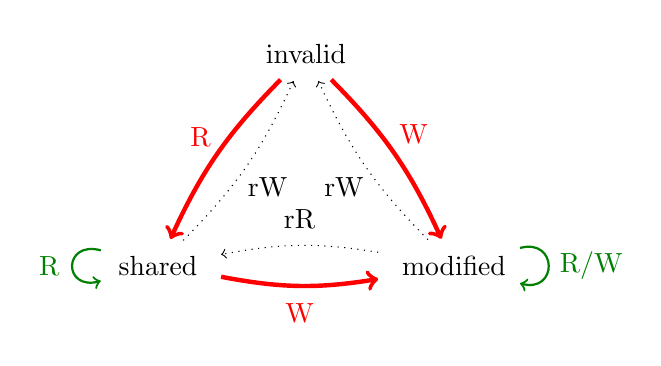
\begin{tikzpicture}[x=2cm,y=2cm,bend angle=10,
%    every node/.style={draw},
    rfo/.style={->,red,ultra thick},
    local/.style={->,green!50!black,thick},
    remote/.style={->,dotted}]

    \begin{scope}[every node/.append style={shape=ellipse}]
      \node (I) at (90:1) {invalid};
      \node (S) at (200:1) {shared};
      \node (M) at (340:1) {modified};
    \end{scope}

    \begin{scope}[every node/.append style={shape=circle,inner sep=2pt}]
      \draw[rfo] (I) to[bend right] node[auto=right] {R} (S);
      \draw[rfo] (I) to[bend left] node[auto=left] {W} (M);

      \draw[rfo] (S) to[bend right] node[auto=right] {W} (M);
      \draw[local,<-] (S) to[loop left,distance=5mm] node {R} (S);
      \draw[remote] (S) to[bend right] node[auto=right] {rW} (I);

      \draw[local] (M) to[loop right,distance=5mm] node {R/W} (M);
      \draw[remote] (M) to[bend left] node[auto=left] {rW} (I);
      \draw[remote] (M) to[bend right] node[auto=right] {rR} (S);
    \end{scope}
  \end{tikzpicture}
  %
  \splitcaption{A basic cache-coherence state machine.}{``R'' and
    ``W'' indicate local read and write operations, while ``rR'' and
    ``rW'' indicate remote read and write operations.  Thick red lines
    show operations that cause communication.  Thin green lines show
    operations that occur without communication.}
  \label{fig:mesi}
\end{figure}

\Cref{fig:mesi} shows the basic state machine implemented by each
cache for each cache line.  This maintains the above invariant by
ensuring a cache line is either invalid in all caches, modified in one
cache and invalid in all others, or shared by any number of caches.
Practical implementations add further states---MESI's ``exclusive''
state, Intel's ``forward'' state~\cite{goodman:mesif}, and AMD's
``owned'' state~\cite[\S7.3]{amd-arch-2}---but these do not change the
basic communication required to maintain cache coherence.

Roughly, a set of operations scales when maintaining coherence does
not require communication in the steady state.
%
Multiple cores reading different cache lines scales because, once each
cache line is in each core's cache, no further communication is
required to access it, so further reads can proceed independently of
concurrent operations.
%
Likewise, multiple cores writing different cache lines scales for much
the same reason.
%
Multiple cores reading the \emph{same} cache line also scales because
the line can be kept in each core's cache in shared mode, allowing
further reads to proceed independently and in parallel with no
coordination.
%
These three conditions are synonymous with conflict-freedom.
%
Furthermore, higher level operations composed of conflict-free reads
and writes are
themselves conflict-free and will also execute independently and in
parallel.
%
In all of these cases, conflict-free operations execute in the same
time in isolation as they do concurrently, so the total throughput of
$N$ such concurrent operations is proportional to $N$.  Therefore,
conflict-free operations scale.

The converse is also true: conflicting operations cause
cache state transitions and the resulting coordination limits
scalability.
%
That is, if a cache line written by one core is read or written by
other cores, those operations must
coordinate and, as a result, will slow each other down.  While this
doesn't directly concern the scalable commutativity rule (which says
only when operations can be conflict-free, not when they must be
conflicted), the huge effect that conflicts can have on scalability
affirms the importance of conflict-freedom.

The following sections verify that conflict-free operations scale
linearly on real hardware, show that conflicts can severely limit
scalability, and explore
the practical limitations of conflict-free scalability.


\subsection{Conflict-free operations scale}
\label{sec:scalability:conflict-free}

We use two machines to evaluate conflict-free and conflicting
operations on real hardware: an 80-core (8 sockets $\times$ 10 cores)
Intel Xeon E7-8870 (the same machine used for evaluation in
\cref{sec:eval}) and, to show that our conclusions generalize, a
48-core (8 sockets $\times$ 6 cores) AMD Opteron 8431.
%
Both are cc-NUMA x86 machines with directory-based cache coherence,
but two manufacturers use different architectures, interconnects, and
coherence protocols.
%
\Cref{fig:machines} shows how the
two machines are broadly organized.

\begin{figure}
  \centering
  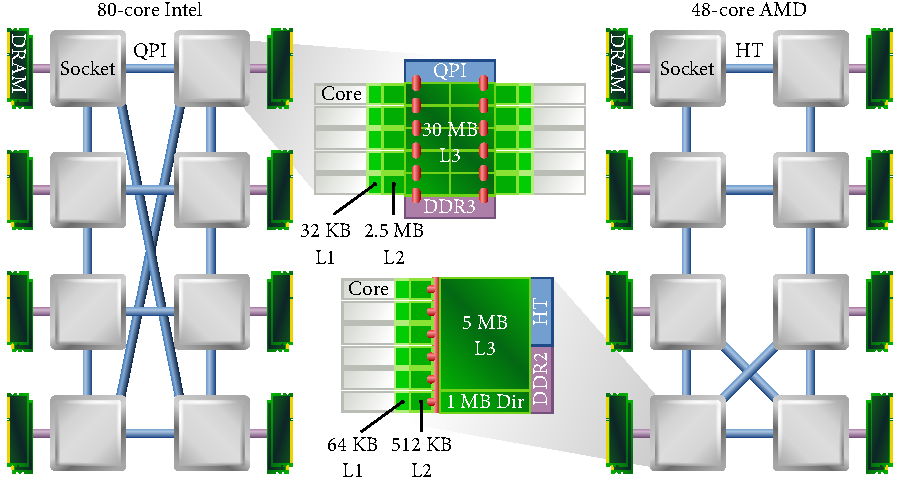
\includegraphics{figures/machines.pdf}
  \caption[Organization of benchmark machines.]{Organization of Intel
    and AMD machines used for
    benchmarks~\cite{ben-motherboard,tom-motherboard-1,tom-motherboard-2}.}
  \label{fig:machines}
\end{figure}

\XXX[AC]{The conflict-free benchmarks wait between accesses.  Maybe
  they should be run at full tilt?}

\begin{figure}
  \centering
  \inputnodraft{graph/cfree-cycles}
  %
  \splitcaption{Conflict-free accesses scale.}{Each graph shows the
    cycles required to perform a conflict-free read or write from $N$
    cores.  Shading indicates the latency distribution for each $N$
    (darker shading indicates higher frequency).}
  \label{fig:cfree-cycles}
\end{figure}

\Cref{fig:cfree-cycles} shows the time required to perform
conflict-free memory accesses from varying numbers of cores.  The
first benchmark, shown in the top row of \cref{fig:cfree-cycles},
stresses read/read sharing by repeatedly reading the same cache line
from $N$ cores.  The latency of these reads remains roughly constant
regardless of $N$.
% (growing slightly on the AMD machine because of increasing noise).
After the first access from each core, the cache
line remains in each core's local cache, so later accesses occur
locally and independently, allowing read/read accesses to scale
perfectly.  Reads of different cache lines from different cores (not
shown) yield identical results to reads of the same cache line.

The bottom row of \cref{fig:cfree-cycles} shows the results of
stressing conflict-free writes by assigning each core a different
cache line and repeatedly writing these cache lines from each of $N$
cores.  In this case these cache lines enter a ``modified'' state at
each core, but then remain in that state, so as with the previous
benchmark, further writes can be performed locally and independently.
%
Again, latency remains constant regardless of $N$, demonstrating that
conflict-free write accesses scale.

\begin{figure}
  \centering
  \inputnodraft{graph/conflict-cycles}
  %
  \splitcaption{Conflicting accesses do not scale.}{Each graph shows
    the cycles required to perform a conflicting read or write from
    $N$ cores.  Shading indicates the latency distribution for each
    $N$ (estimated using kernel density estimation).}
  \label{fig:conflict-cycles}
\end{figure}

\Cref{fig:conflict-cycles} turns to the cost of conflicting
accesses.  The top row shows the latency of $N$ cores writing the same
cache line simultaneously.  The cost of a write/write conflict grows
dramatically as the number of writing cores increases because
ownership of the modified cache line must pass to each writing
core, one at a time.  On both machines, we also see a uniform
distribution of write latencies, which further illustrates this
serialization, as some cores acquire ownership quickly, while others
take much longer.

For comparison, a single complex system call like \code{open}
typically takes 1,000--2,000 cycles on these machines, while a single
conflicting write can take upwards of 50,000 cycles.
%
In the time it takes one thread to perform a single write to a highly
contended cache line, another could open 25 files.

% On the AMD machine, the growth of the mean latency and the spread of
% the distribution are noticeably super-linear as the benchmark adds
% cores further from core 0.

The bottom row of \cref{fig:conflict-cycles} shows the latency of $N$
cores simultaneously reading a cache line last written by core 0 (a
read/write conflict).  For the AMD machine, the results are nearly
identical to the write/write conflict case, since this machine
serializes requests for the cache line at CPU 0's socket.  On the
Intel machine, the cost of read/write conflicts also grows, albeit
more slowly, as Intel's architecture aggregates the read requests at
each socket.
%
We see this effect in the latency distribution, as well, with read
latency exhibiting up to eight different modes.  These modes reflect
the order in which the eight sockets' aggregated read requests are
served by CPU 0's socket.
% (notably, all sockets exhibit all modes, so this is not simply an
% effect of distance from the home socket).
Intel's optimization helps reduce the absolute
latency of reads, but nevertheless, read/write conflicts do not scale
on either machine.


\subsection{Limitations of conflict-free scalability}
\label{sec:scalability:limits}

Conflict-freedom is a good predictor of scalability on real hardware,
but it's not perfect.  Limited cache capacity and associativity cause
caches to evict cache lines (later resulting in cache
misses) even in the absence of coherence traffic.
%
And, naturally, a core's
very first access to a cache line will miss.  Such misses directly
affect sequential performance, but they may also affect the
scalability of conflict-free operations.
%
Satisfying a cache miss (due to conflicts or capacity) requires the
cache to fetch the cache line from another cache or from memory.
%
If this requires communicating with remote cores or remote memory, the
fetch may contend with concurrent operations for interconnect
resources or the remote memory controller.

Applications with good cache behavior are unlikely to exhibit such
issues, while applications with poor cache behavior usually have
sequential performance problems that outweigh scalability concerns.
Nevertheless, it's important to understand where our assumptions about
conflict-freedom break down.

\begin{figure}
  \centering
  \inputnodraft{graph/memscan}
  %
  \splitcaption{Operations scale until they exceed cache or directory
    capacity.}{Each graph shows the latency for repeatedly reading a
    shared region of memory (top) and writing separate per-core
    regions (bottom), as a function of region size and number of
    cores.}
  \label{fig:memscan}
\end{figure}

\Cref{fig:memscan} shows the results of a benchmark that explores some
of these limits by performing conflict-free accesses to regions of
varying sizes from varying numbers of cores.
%
This benchmark stresses the worst case: each core reads or writes in a
tight loop and all memory is physically allocated from CPU 0's socket,
so all misses contend for that socket's resources.
%
The top row of \cref{fig:memscan} shows the latency of reads to a
shared region of memory.
%
On both
machines, we observe slight increases in latency as the region exceeds
the L1 cache and later the L2 cache, but the operations continue to
scale until the region exceeds the L3 cache.  At this point the
benchmark becomes bottlenecked by the DRAM controller of CPU 0's
socket, so the reads no longer scale, despite being conflict-free.

We observe a similar effect for writes, shown in the bottom row of
\cref{fig:memscan}.  On the Intel machine, the operations scale until
the combined working set of the cores on a socket exceeds the socket's
L3 cache size.  On the AMD machine, we observe an additional
effect for smaller regions at high core counts: in this machine,
each socket has a 1~MB directory for tracking ownership of that
socket's physical memory, which this benchmark quickly exceeds.
% The Intel machine has a similar directory, but it's integrated into
% the L3~\cite{intel:e7-8870} and sufficiently provisioned even for
% this benchmark.

\XXX[AC]{False sharing is another common limitation.}


\subsection{Summary}

Despite some limitations, conflict-freedom remains a good predictor
of scalability in practice.  Most software has good cache locality and
high cache hit rates both because this is crucial for sequential
performance, and because it's in the interest of CPU manufacturers to
design caches that fit typical working sets.  For workloads that
exceed cache capacity, NUMA-aware allocation spreads physical memory
use across sockets and DRAM controllers, partitioning physical memory
access, distributing the DRAM bottleneck, and giving cores greater
aggregate DRAM bandwidth.

\Cref{sec:eval} will return to hard numbers on real hardware to show
that conflict-free implementations of commutative interfaces enable
software to scale not just at the level of memory microbenchmarks, but
at the level of an entire OS kernel and its applications.

\XXX[AC]{Conclude by saying that we now have the rule in its full,
  pragmatic form?}

\XXX![FK]{Should this section cite some other performance studies?
  E.g., ``these results are consistent with that other SOSP paper in
  your session.''}

% Causes home node access.  If the missing core is not the line's home
% node, then it has to make a remote request, which takes longer
% depending on how far away the remote node is and can contend for
% interconnect and the remote memory controller.  Even if a core
% misses on a local line, it may contend with other cores on the same
% node for resources.

% Assume some cache locality so compulsory misses are rare (enough to
% keep DRAM bandwidth demand within the capacity of the hardware),
% NUMA-aware memory allocation so that, when there is a miss, it can
% generally be serviced locally.  Such optimizations are standard
% practice, as they are important for sequential performance as they
% are for scalability.


% In the abstract model, two types of memory access scale:
% different cores reading the same read-only memory,
% and different cores writing distinct memory locations.
% Figure~\ref{fig:read-scaling} shows the costs of performing these two types of
% operations simultaneously from 6~cores, 24~cores, and 48~cores.  This benchmark
% stresses the worst case: all memory is physically allocated from NUMA node 0
% and each core reads or writes memory in a tight loop.  The behavior
% depends on how much memory is used by each core.  In both cases, the
% operations scale perfectly until the combined working set on a chip exceeds
% that chip's L3 cache.  After this, the benchmark is bottlenecked by
% node 0's DRAM controller, which can be saturated by even a single chip.  This
% indicates that physical hardware agrees with our abstract model for working sets
% that fit in cache.  Beyond this, hardware does not scale, though in practice
% NUMA-aware allocation and lower bandwidth requirements lessen the impact of
% overflowing the cache.

\section{Designing commutative interfaces}
\label{sec:posix}

\XXX[STATUS]{Unchanged from SOSP.  No changes planned.}

\noindent
The rule facilitates scalability reasoning at the interface and
specification level, and \SIM\ commutativity lets us apply the rule to
complex interfaces.
%\Cref{sec:topic:strong-commutativity} gave a glimpse of this using
%\code{open}.
\Thiscref{sec:posix} demonstrates the interface-level reasoning enabled by the
rule. Using POSIX as a case study, we explore changes that make operations
commute in more situations, enabling more scalable implementations.
%
Already, many POSIX operations commute with many other
operations, a fact we will quantify in the next \lcnamecref{sec:tool};
\thiscref{sec:posix} focuses on
problematic cases to give a sense of the subtler issues of commutative
interface design.
%
% While the details here are specific to POSIX, the general ideas are
% applicable to any interface.

\paragraph{Decompose compound operations.}

Many POSIX APIs combine several operations into one, limiting the
combined operation's commutativity.
For example,
\code{fork} both creates a new process and snapshots the current process's
entire memory state, file descriptor state, signal mask, and several
other properties.  As a result, \code{fork} fails to commute
with most other operations in the same process, such as memory writes,
address space operations, and many file descriptor operations.
However, applications often follow \code{fork} with
\code{exec}, which undoes most of \code{fork}'s sub-operations.
With only \code{fork} and \code{exec}, applications are forced to accept
these unnecessary sub-operations that limit commutativity.

POSIX has a little-known API called \code{posix_spawn} that
addresses this problem by creating a process and loading an image
directly (\code{CreateProcess} in Windows is similar).  This is
equivalent to \code{fork}/\code{exec}, but its specification eliminates
the intermediate sub-operations.  As a result, \code{posix_spawn}
commutes with most other operations and permits a broadly scalable
implementation.
% As we show in \cref{sec:eval:app}, using \code{posix_spawn} instead of
% \code{fork} and \code{exec} leads to better scalability.

Another example, \code{stat}, retrieves and returns many
different attributes of a file simultaneously, which makes it
non-commutative with operations on the same file that change any
attribute returned by \code{stat} (such as \code{link}, \code{chmod},
\code{chown}, \code{write}, and even \code{read}).  In practice,
applications invoke \code{stat} for just one or two of the returned
fields. An alternate API that gave applications
control of which field or fields were returned
would commute with more operations and enable a more scalable
implementation of \code{stat}, as we show in
\cref{sec:eval:fs-microbenchmarks}.

POSIX has many other examples of compound return values.
\code{sigpending} returns all pending signals, even if the caller only
cares about a subset;
% \code{wait} returns all children, even if the caller
% just cares about a subset;
and \code{select} returns all ready file
descriptors, even if the caller needs only one ready FD.

\XXX[AC]{Examples of weird return values that distinguish things in
pointless ways?  I think open had something annoying with this.}

% \XXX[AC]{Embrace non-determinism?  Embrace under-specification?  Maybe
% this is really about naming.  Do not constrain resource names?  Name
% resources non-deterministically?  Use opaque resource names?}

\paragraph{Embrace specification non-determinism.}

POSIX's ``lowest available FD'' rule is a classic example of
overly deterministic design that results in poor scalability.
Because of this rule, \code{open} operations in the same process (and
any other FD allocating operations) do not commute, since the order in
which they execute determines the returned FDs.  This constraint is rarely
needed by applications and an alternate interface
that could return any
unused FD would allow FD allocation operations to commute and enable
implementations to use well-known scalable allocation methods.  We will
return to this example, too, in \cref{sec:eval:fs-microbenchmarks}.
Many other POSIX interfaces get this right: \code{mmap} can
return any unused virtual address and \code{creat} can assign any unused
inode number to a new file.

% \XXX[AC]{Linearizable interfaces are really the problem below.
% Communication interfaces should allow causal or unconstrained ordering.}

\paragraph{Permit weak ordering.}

Another common source of limited commutativity is strict ordering
requirements between operations.  For many operations, ordering is
natural and keeps interfaces simple to use; for example, when one thread
writes data to a file, other threads can immediately read that data.
%
Synchronizing operations like this are naturally non-commutative.
%
Communication interfaces, on the other hand, often enforce strict
ordering, but may not need to.
For instance, most systems order all messages sent via a local Unix
domain socket, even when using
\code{SOCK_DGRAM}, so any \code{send} and \code{recv} system
calls on the same socket do not commute (except in error conditions).
This is often unnecessary, especially in multi-reader or multi-writer
situations, and an alternate interface that does not enforce ordering
would allow \code{send} and \code{recv} to commute as long as there is
both enough free space and enough pending messages on the socket, which
would in turn allow an implementation of Unix domain sockets to support
scalable communication (which we use in \cref{sec:eval:app}).
% \XXX[AC]{Should be ``as we demonstrate'', but we don't isolate unordered
% sockets.}

% \XXX[AC]{Delay?  Decouple and delay?  Enable asynchrony?  Decouple
% asynchronous operations?  Maybe this should be part of decompose
% compound operations because we're splitting the initiation from the
% final action?  Or part of weak ordering because these operations should
% be weakly ordered with respect to other cores.  This also involves
% specification non-determinism, but in the same way weak ordering does.
% Release resources asynchronously?  Really it's about resources that are
% coordinated with other cores.  Coordinate asynchronously?  The above is
% about coordinate you want to be immediate, just unordered.  This is
% about coordination that can be delayed.}

\paragraph{Release resources asynchronously.}

% \XXX[AC]{kill isn't very compelling.  Others are better.}
% Another example of strict ordering is \code{kill}, which requires that
% the signal be immediately delivered to the target (if it is not masked).
% This means \code{kill} does not commute with the target executing
% instructions.  A delayed \code{kill} would commute with target execution
% and other operations, and would
% allow a kernel to batch signal delivery.

A closely related problem is that many POSIX operations have global
effects that must be visible before the operation returns.
This is generally good design for usable interfaces, but for
operations that release resources, this is often stricter than
applications need and expensive to ensure.  For example, writing
to a pipe
must deliver \code{SIGPIPE} immediately if there are no
read FDs for that pipe, so pipe writes do not commute with the last
\code{close}
of a read FD.  This requires aggressively tracking the number of
read FDs; a relaxed specification that promised to eventually deliver the
\code{SIGPIPE} would allow implementations to use more scalable
read FD tracking.
Similarly, \code{munmap} does not commute
with memory reads or writes of the unmapped region from other threads.
Enforcing this requires non-scalable remote TLB shootdowns before \code{munmap}
can return, even though depending
on this behavior usually indicates a bug.  An \code{munmap} (perhaps an
\code{madvise}) that released virtual memory asynchronously
would let the kernel
reclaim physical memory lazily and batch or eliminate remote TLB
shootdowns.


% \section{Example}
\label{sec:example}

This section illustrates ways in which the commutativity rule helps
designers think about implementations, using reference counters as a
case study.

Consider a reference counter with three operations, \OP{inc}, \OP{dec},
and \OP{check}.
%
The \OP{inc} operation increments the reference count and returns
\OK.
%
The \OP{dec} operation decrements the reference count and returns
\OK.
%
Finally, the \OP{check} operation returns \TRUE\ if the count is
non-positive and \FALSE\ otherwise.
%
The intent is that a client calls \OP{inc} when obtaining a reference
and \OP{dec} when releasing a reference.  At some point, possibly after
many \OP{inc} and \OP{dec} operations, the client
calls \OP{check}, freeing the object if \OP{check} returns \TRUE.

An obvious way in which this interface commutes is that \OP{inc} and
\OP{dec} operations commute with themselves and each other. This
observation can be turned into a scalable implementation by splitting
(or partitioning) the counter representation: giving each core a
separate counter, with the abstract counter equal to the sum
of the per-core counters. \OP{inc} and \OP{dec} operate on the local
per-core counter, while \OP{check} must take the sum of the per-core
counters~\cite{XXX}. This splitting is a common and long-standing
pattern for scalable implementations, evident in techniques such as
per-core free lists~\cite{XXX}.

Applying the commutativity rule shows there at least one more scaling
possibility.
Consider the following six-thread history, with an initial
count of 3:
%
\begin{align*}
\HIST{H} = [& \INV{check}{}{1}, \RES{check}{\FALSE}{1}, ~~
	      \INV{check}{}{2}, \RES{check}{\FALSE}{2}, ~~
	      \INV{dec}{}{3}, \RES{dec}{\OK}{3}, \\
            & \INV{dec}{}{4}, \RES{dec}{\OK}{4}, ~~
	      \INV{dec}{}{5}, \RES{dec}{\OK}{5}, ~~
              \INV{check}{}{6}, \RES{check}{\TRUE}{6}].
\end{align*}
%
Although in general \OP{check} operations do not commute with \OP{inc}
or \OP{dec} operations, in this history, the first four operations
commute (the first two \OP{check}s and the first two \OP{dec}s).
%
And a different partitioning of the abstract counter shows these
operations can be implemented scalably as well.
%
Each core would maintain a per-core counter 
  (whose sum is one
  less than the true counter) and a
  per-core \OP{check} snapshot, which is defined to
  \TRUE\ iff the sum of the per-core counters is negative. A \OP{dec}
  call decrements its per-core counter. If the per-core counter goes
  negative, the \OP{dec} call must read and sum all the counters and update
  the \OP{check} snapshots accordingly.
  In this history, threads 3 and 4 might start out with per-core
  counters equal to 1, with thread 5's per-core counter equal to 0.
  Then the first four operations will execute scalably.
  %
  The operations would not execute scalably given other
  initial per-core counter assignments.

The two scalable implementations described are fundamentally different.
Which is most desirable depends on whether the workload is
expected to be write-heavy (mostly \OP{inc} and \OP{dec}) or
read-heavy (mostly \OP{check}).
Thus an implementer must determine what opportunities to scale exist,
then decide which are likely to be the most valuable,
then choose the implementation that scales in those situations.

As an example of how the commutativity rule can help in choice
of interface, consider a slightly different reference counter
with a \OP{deccheck} operator that decrements the counter
and returns
\TRUE\ if the decrement caused the counter to become non-positive.
%
Linux's \verb+atomic_inc+ and \verb+atomic_dec_and_test+
functions provide this kind of interface.
%
Commutativity reasoning shows how this interface choice limits
scalability.
%
A history with three decrements would look like this:
%
\begin{align*}
\HIST{H'} = [&\INV{deccheck}{}{3}, \RES{deccheck}{\FALSE}{3}, ~~
	     \INV{deccheck}{}{4}, \RES{deccheck}{\FALSE}{4}, \\
             &\INV{deccheck}{}{5}, \RES{deccheck}{\TRUE}{5}]
\end{align*}
%
Unlike the three \OP{dec} operations in $H$ above, the three
\OP{deccheck} operations in $H'$ \emph{do not}
commute.
%
The interface with combined decrement is harder to make scale than
the interface that separates decrement from checking.
%
On the other hand, if, in most histories, the counter has a large
positive value, then even the \OP{deccheck} interface commutes, and
therefore can be made to scale using per-core counters.

% In practice, designers make trade-offs between scalability
% and other desired properties.  For example, memory is not
% unlimited, so the kernel must reuse memory; but re-using memory that has been used
% by an operation is not commutative with that operation. As another example, an
% implementation that scales linearly may not be the
% highest performing implementation for a particular core count; e.g.,
% some implementations of a scalable reference counter may be inefficient for a
% small number of cores.

\XXX[EK]{Would like to wrap up the point of this section here.}

\XXX[nz]{Simple POSIX file system example.}



\section{Analyzing interfaces using \tool}
\label{sec:tool}

\XXX[STATUS]{\analyzer section rewritten from SOSP.  Planning to
  expand \testgen section a bit.
  Applied: Minor edits from Eddie init-244-ga695479.
  Unapplied: Eddie init-244-ga695479.
}

Fully understanding the commutativity of a complex interface is
tricky, and achieving an
implementation that avoids sharing when operations commute adds another
dimension to an already difficult task.  However, by leveraging the
formality of the commutativity rule, developers can automate much of this
reasoning.  \Thiscref{sec:tool} presents a systematic, test-driven approach to
applying the commutativity rule to real implementations embodied in a
tool named \tool, whose components are shown in
\cref{fig:tool}.


\begin{figure*}
\section{Analyzing interfaces using \tool}
\label{sec:tool}

\XXX[STATUS]{\analyzer section rewritten from SOSP.  Planning to
  expand \testgen section a bit.
  Applied: Minor edits from Eddie init-244-ga695479.
  Unapplied: Eddie init-244-ga695479.
}

Fully understanding the commutativity of a complex interface is
tricky, and achieving an
implementation that avoids sharing when operations commute adds another
dimension to an already difficult task.  However, by leveraging the
formality of the commutativity rule, developers can automate much of this
reasoning.  \Thiscref{sec:tool} presents a systematic, test-driven approach to
applying the commutativity rule to real implementations embodied in a
tool named \tool, whose components are shown in
\cref{fig:tool}.


\begin{figure*}
\section{Analyzing interfaces using \tool}
\label{sec:tool}

\XXX[STATUS]{\analyzer section rewritten from SOSP.  Planning to
  expand \testgen section a bit.
  Applied: Minor edits from Eddie init-244-ga695479.
  Unapplied: Eddie init-244-ga695479.
}

Fully understanding the commutativity of a complex interface is
tricky, and achieving an
implementation that avoids sharing when operations commute adds another
dimension to an already difficult task.  However, by leveraging the
formality of the commutativity rule, developers can automate much of this
reasoning.  \Thiscref{sec:tool} presents a systematic, test-driven approach to
applying the commutativity rule to real implementations embodied in a
tool named \tool, whose components are shown in
\cref{fig:tool}.


\begin{figure*}
\input{figures/tool.tex}
\caption{The components of \tool. \XXX![AC]{Fix overfull hbox.}}
\label{fig:tool}
\end{figure*}

First, \analyzer takes a symbolic model of
an interface and computes precise conditions under which that interface's
operations commute.  Second, \testgen takes
these conditions and generates concrete test cases of sets of operations
that commute according to the interface model, and thus should
have a conflict-free implementation according to the commutativity rule.
%
Third, \mtrace checks whether a particular implementation is
conflict-free for each test case.

A developer can use these test cases to understand the
commutative cases they should consider,
to iteratively find and fix scalability
issues in their
code, or as a regression test suite to ensure
scalability bugs do not creep into the implementation over time.


\subsection{\analyzer}
\label{sec:tool:analyzer}

% Alternate outline: Step through in detail with two operations,
% following commutes2 algorithm, then generalize to sets of operations
% in the obvious way, then discuss $n$-cube optimization.  Need to
% cover 1) how to get from the path conditions to the commutativity
% condition, 2) how \code{commutes} differs from SIM commutativity,
% and 3) how we implement ``internal'' variables.  Also need to
% explain (preferably early) how this connects to SIM commutativity:
% that the unconstrained initial state represents all possible
% histories that could come before the operations under test and that
% testing for final state equivalence tests whether any future $Z$ can
% distinguish the different orders.  This keeps things grounded in
% examples from the start, but front-loads symbolic execution and
% separates the rename example from the transition into testgen.


\analyzer automates the process of analyzing the commutativity of an
interface, saving developers from the tedious and error-prone process of
considering large numbers of interactions between complex operations.
%
\analyzer takes as input a model of the behavior of an interface,
written in a symbolic variant of Python, and outputs \emph{commutativity
  conditions}: expressions in terms of arguments and state for exactly
when sets of operations commute.
%
A developer can inspect these expressions to understand an interface's
commutativity or pass them to \testgen (\cref{sec:tool:generator})
to generate concrete examples of when interfaces commute.

% Diagrammatically, something like:
%                        /- op_b=>r_ab @ S_ab -- op_c=>r_abc @ S_abc
%       / op_a=>r_a @ S_a
%      /                 \- op_c=>r_ac @ S_ac -- op_b=>r_acb @ S_acb
%     /                  /- op_a=>r_ba @ S_ba -- op_c=>r_bac @ S_bac
% S_0 --- op_b=>r_b @ S_b
%     \                  \- op_c=>r_bc @ S_bc -- op_a=>r_bca @ S_bca
%      \                 /- op_a=>r_ba @ S_ca -- op_b=>r_cab @ S_cab
%       \ op_c=>r_c @ S_c
%                        \- op_b=>r_bc @ S_cb -- op_a=>r_cba @ S_cba
%
%   (r_a == r_ba == r_bca == r_ca == r_cba) /\
%   (r_b == r_ab == r_acb == r_cab == r_cb) /\
%   (r_c == r_abc == r_ac == r_bac == r_bc) /\
%   (S_ab == S_ba) /\ (S_ac == S_ca) /\ (S_bc == S_cb) /\
%   (S_abc == S_acb == S_bac == S_bca == S_cab == S_cba)
%
% See also [[2013-08-21 :SCP Analyzer pseudo-code]]
%
% Actually, many of these comparisons are redundant.  See the whiteboard
% photo from 2013-09-14.

Given the Python code for a model, \analyzer uses symbolic execution to
consider all possible behaviors of the interface model and construct
complete commutativity conditions.  Symbolic execution also enables
\analyzer to reason about the external behavior of an interface, rather
than specifics of the model's implementation, and enables models to
capture specification non-determinism (like \code{creat}'s ability to
choose any free inode) as under-constrained symbolic values.

% Larger sets are exponentially more expensive: An n-cube has n *
% 2^(n-1) edges, so each individual commutativity test is exponential
% in the number of operations (symbolic branching probably makes this
% doubly exponential, and the growing path condition at least adds a
% polynomial factor and may add another exponential).  The number of
% tests we need to do is nCr(n + k - 1, k) where n is the number of
% interface operations and k is the number under test.  This probably
% makes it triply exponential, but I'm not sure what the growth in k
% is.

\subsubsection{Concrete commutativity analysis}

Starting from an interface model, \analyzer computes the commutativity
condition of each multiset of operations of a user-specified size.
%
To determine whether a set of operations commutes, \analyzer executes
the SIM commutativity test algorithm given in \cref{fig:commutes}.  To
begin with, we can think of this test in concrete (non-symbolic) terms
as a test of whether a set of operations commutes starting from a
specific initial state \code{s0} and given specific operation
arguments \code{args}.

\begin{figure}
  \inputcode{code/commutes}
  %
  \splitcaption{The \SIM commutativity test algorithm.}{\code{s0} is
    the initial state, \code{ops} is the list of operations to test
    for commutativity, and \code{args} gives the arguments to pass to
    each operation.  For clarity, this implementation assumes all
    values in ops are distinct.}
  \label{fig:commutes}
\end{figure}

% Alternate code:
% def commutes(s0, ops, args):
%   results, states = {}, {}
%   for perm in permutations(ops):
%     s = s0.copy()
%     for i, op in enumerate(perm):
%       r = op(s, args[op])
%
%       # Test result equivalence
%       if op not in results:
%         results[op] = r
%       elif r != results[op]:
%         return False
%
%       # Test state equivalence
%       op_set = frozenset(perm[:i+1])
%       if op_set not in states:
%         states[op_set] = s.copy()
%       elif s != states[op_set]:
%         return False
%  return True

This test is implemented by a function called \code{commutes}.
\code{commutes} codifies the definition of \SIM commutativity, except
that it requires the specification to be sequentially consistent so it
needn't interleave partial operations.  Recall that $\HY$ \SI-commutes
in $H = \HX \HCONCAT \HY$ when, given any reordering $\HY'$ of $\HY$
and any action sequence $\HSUFF$, \[\HX \HCONCAT \HY \HCONCAT \HSUFF
\in \SPEC \text{~~~if and only if~~~} \HX \HCONCAT \HY' \HCONCAT
\HSUFF \in \SPEC.\]  Further, for $\HY$ to \SIM-commute in $H$, every
prefix of every reodering of $\HY$ must \SI-commute.
%
In \code{commutes}, the initial state \code{s0} serves the role of the
prefix $\HX$: to put the system in some state.
% For alternate code:
% The outer loop of \code{commutes} considers all reorderings ($\HY'$)
% of the operations under test (assuming sequential consistency).  The
% inner loop executes each individual reordering and performs a result
% test and a state test.
\code{ops} serves the role of $\HY$ (assuming sequential consistency)
and the loop in \code{commutes} generates every $\HY'$, that is, all
prefixes of all reoderings of $\HY$.  This loop performs two tests.
First, the result equivalence test ensures that each operation gives
the same response in all reorderings.  Finally, the state equivalence
test serves the role of the future actions, $\HSUFF$, by requiring all
prefixes of all reorderings to converge on states that are
indistinguishable by future operations.

Since \code{commutes} substitutes state equivalence in place of
considering all possible future operations (which would be difficult
with symbolic execution), it's up to the model's author to define
state equivalence as whether two states are externally
indistinguishable.  This is standard practice for high-level data
types (e.g., two sets represented as trees could be equal even if they
are balanced differently).  For the POSIX model we present in
\cref{sec:topic:model}, only a few types need special handling beyond what
\analyzer's high-level data types already provide.

The \code{commutes} algorithm can be optimized by observing that if
two permutations of the same prefix reach the same state, only one
needs to be considered further.  This optimization gives
\code{commutes} a pleasing symmetry: it becomes equivalent to
exploring all $n$ step paths from $\tup<0,0,\ldots>$ to
$\tup<1,1,\ldots>$ in an $n$-cube, where each unit step is an
operation and each vertex is a state.


\subsubsection{Symbolic commutativity analysis}
\label{sec:topic:rename-conditions}

So far, we've considered only how to determine if a set of operations
commutes for a specific initial state and specific arguments.
Ultimately, we're interested in the entire space of states and
arguments for which a set of operations commutes.  To find this,
\analyzer executes \code{commutes} \emph{symbolically}, passing it an
unconstrained symbolic initial state and unconstrained symbolic
operation arguments.  Symbolic execution lets \analyzer efficiently
consider \emph{all possible} initial states and arguments and
precisely determine the (likely infinite) set of states and arguments
for which the operations commute (that is, for which \code{commutes}
returns \code{True}).

\begin{figure}
  \inputcode{code/rename}
  \caption{A simplified version of our \code{rename} model.}
  \label{fig:rename-spec}
\end{figure}

\Cref{fig:rename-spec} gives an example of how a developer could model
the \code{rename} operation in \analyzer.  The first five lines
declare symbolic types used by the model (\code{tuninterpreted}
declares a type whose values support only equality).  The \code{POSIX}
class, itself a symbolic type, represents the \emph{system state} of
the file system and its methods implement the interface operations to
be tested.  The implementation of \code{rename} itself is
straightforward.  Indeed, the familiarity of Python and ease of
manipulating state were part of why we chose it over abstract
specification languages.

% \begin{figure}
%   \inputcode{code/commutes2-old}
%   \splitcaption{The \SIM commutativity test algorithm for two
%     operations.}{\tool executes \code{commutes} symbolically and
%     \code{commutes} executes the operations being tested.  Given a
%     system state type and two operations, \code{commutes} returns
%     whether the operations commute under the constraints of the path
%     condition that leads to the return.}
%   \label{fig:commutes2-old}
% \end{figure}
\begin{figure}
  \inputcode{code/commutes2}
  \caption{The \SIM commutativity test algorithm specialized to two
    operations.}
  \label{fig:commutes2}
\end{figure}

To explore how \analyzer analyzes \code{rename}, we'll use the version
of \code{commutes} given in \cref{fig:commutes2}, which is specialized
for pairs of operations.  In practice, we typically analyze pairs of
operations rather than larger sets because larger sets take
exponentially longer to analyze and rarely reveal problems beyond
those already revealed by pairs.

% Derived from figures/tree.tex
\newcommand\treecommutes{%
  \tikz[y=-0.0111111in,x=0.0111111in]{
    \definecolor{tmpfill}{rgb}{0,1,0}
    \path[fill=tmpfill] (0,0) circle (4.29);
    \node[font=\fontsize{5}{6}\selectfont,text=white,inner sep=0pt] {$\checkmark$};
  }%
}
\newcommand\treediverges[1]{%
  \tikz[y=-0.0111111in,x=0.0111111in]{
    \definecolor{tmpfill}{rgb}{1,0,0}
    \path[fill=tmpfill] (0,0) circle (4.29);
    \node[font=\fontsize{5}{6}\selectfont,text=white,inner sep=0pt] {#1};
  }%
}
\begin{figure}
  \centering
  \inputnodraft{figures/tree.tex}
  %
  \splitcaption{Symbolic execution tree of \code{commutes2} for
    \code{rename/rename}.}{Each node represents a conditional branch
    on a symbolic value.  The terminals at the right indicate whether
    each path constraint yields a commutative execution of the two
    operations (\treecommutes), or, if not, whether it diverged on
    return values (\treediverges{R}) or final state
    (\treediverges{S}).}
  \label{fig:rename-branching}
\end{figure}

\XXX[AC]{Add line labels to figure that match up with code listings?}

\XXX[AC]{Show initial path condition and some final path conditions in
  figure?}

\Cref{fig:rename-branching} illustrates the symbolic execution of
\code{commutes2} testing a pair of \code{rename} operations.
%
By and large, this symbolic execution proceeds like regular Python
execution, except when it encounters a conditional branch on a
symbolic value (such as any \code{if} statement in \code{rename}).
Symbolic execution always begins with an empty symbolic \emph{path
  condition}.  To execute a conditional branch on a symbolic value,
\analyzer uses an SMT solver to determine whether that symbolic value
can be true, false, or either, given the path condition accumulated so
far.
%
If the branch can go both ways, \analyzer logically forks the symbolic
execution and extends the path conditions of the two forks with the
constraints that the symbolic value must be true or false,
respectively.  These growing path conditions thereby constrain further
execution on the two resulting code paths.

The four main regions of \cref{fig:rename-branching} correspond to the
four calls to \code{rename} from \code{commutes2} as it tests the two
different reorderings of the two operations.  Each call region shows
the three conditional branches in \code{rename}.  The first call forks
at every conditional branch because the state and arguments are
completely unconstrained at this point; \analyzer therefore explores
every code path through \code{rename}.  The second call forks
similarly.  The third and fourth calls generally do not fork; by this
point, the symbolic values of \code{s0}, \code{argsA}, and
\code{argsB} are heavily constrained by the path condition produced by
the first two calls.  As a result, these calls are often forced to
make the same branch as the corresponding earlier call.

Finally, after executing both reorderings of \code{rename/rename},
\code{commutes2} tests their commutativity by checking if each
operation's return value is equivalent in both permutations and if the
system states reached by both permutations are equivalent.  This, too,
is symbolic and may fork execution if it's still possible for the pair
of operations to be either commutative or non-commutative (we see a
couple such forks in \cref{fig:rename-branching}).

Together, the set of path conditions that pass this final
commutativity test are the commutativity condition of this pair of
operations.  Barring SMT solver time-outs, the disjunction of the path
conditions for which \code{commutes2} returns \code{True} captures the
precise set of initial system states and operation arguments for which
the operations commute.

\XXX!{Fix up flow here.}

Given two
\code{rename} operations, \code{rename(a, b)} and \code{rename(c, d)},
\analyzer outputs that they commute if any of the following hold:

\begin{CompactItemize}
\item Both source files exist, and the file names are all different
      (\code{a} and \code{c} exist, and \code{a}, \code{b}, \code{c},
      \code{d} all differ).

\item One \code{rename}'s source does not exist, and it is not the
      other \code{rename}'s destination (either
      \code{a} exists, \code{c} does not, and \code{b}$\neq$\code{c}, or
      \code{c} exists, \code{a} does not, and \code{d}$\neq$\code{a}).

\item Neither \code{a} nor \code{c} exists.

\item Both calls are self-renames (\code{a}$=$\code{b} and \code{c}$=$\code{d}).

\item One call is a self-rename of an existing file
      (\code{a} exists and \code{a}$=$\code{b}, or
       \code{c} exists and \code{c}$=$\code{d}) and
      it's not the other call's source (\code{a}$\neq$\code{c}).

\item Two hard links to the same inode are renamed to the same new name
      (\code{a} and \code{c} point to the same inode,
       \code{a}$\neq$\code{c}, and \code{b}$=$\code{d}).

\end{CompactItemize}

\XXX![AC]{Make point here that we would only have been able to find
  one of these cases without a state-sensitive definition of
  commutativity?}

As this example shows, when system calls access shared, mutable
state, reasoning about every commutative case by hand can become
difficult.
%
Developers can easily overlook cases, both in their
understanding of an interface's commutativity, and when making their
implementation scale for commutative cases.
%
\analyzer
automates reasoning about all possible system states, all possible
sets of operations that can be
invoked, and all possible arguments to those operations.

\XXX[AC]{Are these examples that enlightening?  Do they just reinforce
the ``corner case'' mentality?

For
example, creating two files in two different directories might appear to
be obviously commutative, but in fact if the file system has exactly one
free inode left, these two operations do not commute.
%
As another example, the \code{open()} and \code{stat()} system calls
generally commute if they refer to different file names, but there are a
number of non-obvious cases: e.g., the two operations do not commute if one
of the files does not exist, the other is a symlink to the first, and
\code{open} is invoked with \code{O_CREAT}; or if one file exists and is
non-empty, the other is a symlink to the first, and \code{open} is invoked
with \code{O_TRUNC}.}


\subsection{\testgen}
\label{sec:tool:generator}

While a developer can examine the commutativity conditions
produced by \analyzer directly, for complex interfaces these formulas
can be large and difficult to decipher.  Further, real implementations
are complex and likely to contain unintentional sharing, even if the
developer understands an interface's commutativity.  \testgen takes
the first step to helping developers apply commutativity to real
implementations by converting \analyzer's commutativity conditions into
concrete test cases.

To produce a test case, \testgen computes
a satisfying assignment for the corresponding commutativity condition.
The assignment specifies concrete values for every symbolic variable in
the model, such as the \code{fname_to_inum} and \code{inodes} data structures
and the \code{rename} arguments shown in \cref{fig:rename-spec}.
\testgen then invokes a model-specific function on the assignment
to produce actual C test case code.  For example, one test
case that \testgen generates is shown in \cref{fig:testgen}.
The test case includes setup code that configures the initial state of
the system and a set of functions to run on different cores. Every
\testgen test case should have a conflict-free implementation.

\begin{figure}
\inputcode{code/testgen}
%
\splitcaption{An example test case for two \code{rename} calls
  generated by \testgen}{for the model in \cref{fig:rename-spec}.}
\label{fig:testgen}
\end{figure}

The goal of these test cases is to expose potential scalability problems
in an implementation, but it is impossible for \testgen to know
exactly what inputs might trigger conflicting memory accesses.  Thus, as a
proxy for achieving good coverage on the implementation, \testgen
aims to achieve good coverage of the Python model.

\XXX[E]{THIS PARAGRAPH IS VERY OPAQUE}
We consider two forms of coverage.
The first is the standard notion of path coverage, which \testgen
achieves by relying on \analyzer's symbolic execution.
%
\analyzer produces a separate path condition for every possible code
path through a set of operations.
%
However, even a single path might encounter conflicts in interestingly
different ways.
%
For example, the code path through two \code{pwrite}s is the
same whether they're writing to the same offset or different offsets,
but the access patterns are very different.
%
To capture different conflict conditions as well as path conditions, we
introduce a new notion called \emph{conflict coverage}.  Conflict coverage
exercises all possible access patterns on shared data structures:
looking up two distinct items from different operations, looking up
the same item, etc.
%
\testgen approximates
conflict coverage by concolically executing \emph{itself}
to enumerate distinct tests for each path condition.  \testgen
starts with the constraints of a path condition from \analyzer, tracks
every symbolic expression forced to a concrete value by the
model-specific test code
generator, negates any equivalent assignment of these expressions from
the path condition, and generates another test, repeating this process
until it exhausts assignments that satisfy the path condition or the SMT
solver fails.  Since
path conditions can have infinitely many satisfying assignments (e.g.,
there are infinitely many calls to \code{read} with different FD numbers
that return \code{EBADF}), \testgen partitions most values in
\emph{isomorphism groups} and considers two assignments equivalent if
each group has the same
pattern of equal and distinct values in both assignments.  For our POSIX
model, this
bounds the number of enumerated test cases.

These two forms of coverage ensure that the test cases
generated by \testgen will cover all possible paths and data structure
access patterns in the model, and to the extent that the implementation
is structured similarly to the model, should achieve good coverage
for the implementation as well.  As we demonstrate in \cref{sec:topic:model},
\testgen produces a total of \pyexpr{mscan.ntestcases} test cases
for our model of \pyexpr{len(mscan.calls)} POSIX
system calls, and these
test cases find scalability issues in the Linux \code{ramfs} file system
and virtual memory system.


\subsection{\mtrace}
\label{sec:tool:mtrace}

Finally, \mtrace runs the test cases generated by \testgen on
a real implementation and checks that the implementation is
conflict-free for every test.  If it finds a violation of the
commutativity rule---a test whose commutative operations are not
conflict-free---it reports which variables were shared and what code
accessed them.
%
For example, when running the
test case shown in \cref{fig:testgen} on a Linux \code{ramfs}
file system, \mtrace reports that the two functions make conflicting
accesses to the \code{dcache} reference count and lock, which limits
the scalability of those operations.

\mtrace runs the entire operating system in a modified version of
qemu~\cite{qemu}.  At the beginning of each test case, it issues a hypercall to
qemu to start recording memory accesses, and then executes the test
operations on different virtual cores.  During test execution,
\mtrace logs all reads and writes by each core, along with
information about the currently executing kernel thread,
to filter out irrelevant conflicts by background threads or
interrupts.  After execution, \mtrace analyzes
the log and reports all conflicting memory accesses, along with the C
data type of the accessed memory location (resolved from
DWARF~\cite{dwarf} information and logs
of every dynamic allocation's type) and stack traces for each conflicting
access.

\subsection{Implementation}
\label{sec:tool:impl}

We built a prototype implementation of \tool's three components.
\analyzer and \testgen consist of
\pyexpr{const['commuter-loc']['analyzer']} lines of Python code,
including the symbolic execution engine, which uses the Z3 SMT
solver~\cite{demoura:z3}
via Z3's Python bindings.
\mtrace consists of \pyexpr{const['mtrace-loc']['qemu-diff']} lines of
code changed in qemu, along with \pyexpr{const['pk-loc']['pk-diff']}
lines of code changed in the guest
Linux kernel (to report memory type information, context switches, etc.).
Another program, consisting of \pyexpr{const['mtrace-loc']['mscan']}
lines of C++ code, processes the
log file to find and report memory locations that are shared between different
cores for each test case.

\XXX[AC]{mtrace's custom DWARF library dwarfs the rest of this at
$\sim$6,500 LOC.}

% \mtrace is implemented on a modified qemu~\cite{qemu}.  We added support
% for hypercalls so that software running within \mtrace can communicate
% events such as variable declarations, call stack switches, and the range
% and type of every memory allocation.  \mtrace also modifies the qemu
% code generator to intercept all loads and stores and to trace additional
% instructions such as \code{call} and \code{ret} to produce call stacks.
% This information is written to a log file.


\caption{The components of \tool. \XXX![AC]{Fix overfull hbox.}}
\label{fig:tool}
\end{figure*}

First, \analyzer takes a symbolic model of
an interface and computes precise conditions under which that interface's
operations commute.  Second, \testgen takes
these conditions and generates concrete test cases of sets of operations
that commute according to the interface model, and thus should
have a conflict-free implementation according to the commutativity rule.
%
Third, \mtrace checks whether a particular implementation is
conflict-free for each test case.

A developer can use these test cases to understand the
commutative cases they should consider,
to iteratively find and fix scalability
issues in their
code, or as a regression test suite to ensure
scalability bugs do not creep into the implementation over time.


\subsection{\analyzer}
\label{sec:tool:analyzer}

% Alternate outline: Step through in detail with two operations,
% following commutes2 algorithm, then generalize to sets of operations
% in the obvious way, then discuss $n$-cube optimization.  Need to
% cover 1) how to get from the path conditions to the commutativity
% condition, 2) how \code{commutes} differs from SIM commutativity,
% and 3) how we implement ``internal'' variables.  Also need to
% explain (preferably early) how this connects to SIM commutativity:
% that the unconstrained initial state represents all possible
% histories that could come before the operations under test and that
% testing for final state equivalence tests whether any future $Z$ can
% distinguish the different orders.  This keeps things grounded in
% examples from the start, but front-loads symbolic execution and
% separates the rename example from the transition into testgen.


\analyzer automates the process of analyzing the commutativity of an
interface, saving developers from the tedious and error-prone process of
considering large numbers of interactions between complex operations.
%
\analyzer takes as input a model of the behavior of an interface,
written in a symbolic variant of Python, and outputs \emph{commutativity
  conditions}: expressions in terms of arguments and state for exactly
when sets of operations commute.
%
A developer can inspect these expressions to understand an interface's
commutativity or pass them to \testgen (\cref{sec:tool:generator})
to generate concrete examples of when interfaces commute.

% Diagrammatically, something like:
%                        /- op_b=>r_ab @ S_ab -- op_c=>r_abc @ S_abc
%       / op_a=>r_a @ S_a
%      /                 \- op_c=>r_ac @ S_ac -- op_b=>r_acb @ S_acb
%     /                  /- op_a=>r_ba @ S_ba -- op_c=>r_bac @ S_bac
% S_0 --- op_b=>r_b @ S_b
%     \                  \- op_c=>r_bc @ S_bc -- op_a=>r_bca @ S_bca
%      \                 /- op_a=>r_ba @ S_ca -- op_b=>r_cab @ S_cab
%       \ op_c=>r_c @ S_c
%                        \- op_b=>r_bc @ S_cb -- op_a=>r_cba @ S_cba
%
%   (r_a == r_ba == r_bca == r_ca == r_cba) /\
%   (r_b == r_ab == r_acb == r_cab == r_cb) /\
%   (r_c == r_abc == r_ac == r_bac == r_bc) /\
%   (S_ab == S_ba) /\ (S_ac == S_ca) /\ (S_bc == S_cb) /\
%   (S_abc == S_acb == S_bac == S_bca == S_cab == S_cba)
%
% See also [[2013-08-21 :SCP Analyzer pseudo-code]]
%
% Actually, many of these comparisons are redundant.  See the whiteboard
% photo from 2013-09-14.

Given the Python code for a model, \analyzer uses symbolic execution to
consider all possible behaviors of the interface model and construct
complete commutativity conditions.  Symbolic execution also enables
\analyzer to reason about the external behavior of an interface, rather
than specifics of the model's implementation, and enables models to
capture specification non-determinism (like \code{creat}'s ability to
choose any free inode) as under-constrained symbolic values.

% Larger sets are exponentially more expensive: An n-cube has n *
% 2^(n-1) edges, so each individual commutativity test is exponential
% in the number of operations (symbolic branching probably makes this
% doubly exponential, and the growing path condition at least adds a
% polynomial factor and may add another exponential).  The number of
% tests we need to do is nCr(n + k - 1, k) where n is the number of
% interface operations and k is the number under test.  This probably
% makes it triply exponential, but I'm not sure what the growth in k
% is.

\subsubsection{Concrete commutativity analysis}

Starting from an interface model, \analyzer computes the commutativity
condition of each multiset of operations of a user-specified size.
%
To determine whether a set of operations commutes, \analyzer executes
the SIM commutativity test algorithm given in \cref{fig:commutes}.  To
begin with, we can think of this test in concrete (non-symbolic) terms
as a test of whether a set of operations commutes starting from a
specific initial state \code{s0} and given specific operation
arguments \code{args}.

\begin{figure}
  \inputcode{code/commutes}
  %
  \splitcaption{The \SIM commutativity test algorithm.}{\code{s0} is
    the initial state, \code{ops} is the list of operations to test
    for commutativity, and \code{args} gives the arguments to pass to
    each operation.  For clarity, this implementation assumes all
    values in ops are distinct.}
  \label{fig:commutes}
\end{figure}

% Alternate code:
% def commutes(s0, ops, args):
%   results, states = {}, {}
%   for perm in permutations(ops):
%     s = s0.copy()
%     for i, op in enumerate(perm):
%       r = op(s, args[op])
%
%       # Test result equivalence
%       if op not in results:
%         results[op] = r
%       elif r != results[op]:
%         return False
%
%       # Test state equivalence
%       op_set = frozenset(perm[:i+1])
%       if op_set not in states:
%         states[op_set] = s.copy()
%       elif s != states[op_set]:
%         return False
%  return True

This test is implemented by a function called \code{commutes}.
\code{commutes} codifies the definition of \SIM commutativity, except
that it requires the specification to be sequentially consistent so it
needn't interleave partial operations.  Recall that $\HY$ \SI-commutes
in $H = \HX \HCONCAT \HY$ when, given any reordering $\HY'$ of $\HY$
and any action sequence $\HSUFF$, \[\HX \HCONCAT \HY \HCONCAT \HSUFF
\in \SPEC \text{~~~if and only if~~~} \HX \HCONCAT \HY' \HCONCAT
\HSUFF \in \SPEC.\]  Further, for $\HY$ to \SIM-commute in $H$, every
prefix of every reodering of $\HY$ must \SI-commute.
%
In \code{commutes}, the initial state \code{s0} serves the role of the
prefix $\HX$: to put the system in some state.
% For alternate code:
% The outer loop of \code{commutes} considers all reorderings ($\HY'$)
% of the operations under test (assuming sequential consistency).  The
% inner loop executes each individual reordering and performs a result
% test and a state test.
\code{ops} serves the role of $\HY$ (assuming sequential consistency)
and the loop in \code{commutes} generates every $\HY'$, that is, all
prefixes of all reoderings of $\HY$.  This loop performs two tests.
First, the result equivalence test ensures that each operation gives
the same response in all reorderings.  Finally, the state equivalence
test serves the role of the future actions, $\HSUFF$, by requiring all
prefixes of all reorderings to converge on states that are
indistinguishable by future operations.

Since \code{commutes} substitutes state equivalence in place of
considering all possible future operations (which would be difficult
with symbolic execution), it's up to the model's author to define
state equivalence as whether two states are externally
indistinguishable.  This is standard practice for high-level data
types (e.g., two sets represented as trees could be equal even if they
are balanced differently).  For the POSIX model we present in
\cref{sec:topic:model}, only a few types need special handling beyond what
\analyzer's high-level data types already provide.

The \code{commutes} algorithm can be optimized by observing that if
two permutations of the same prefix reach the same state, only one
needs to be considered further.  This optimization gives
\code{commutes} a pleasing symmetry: it becomes equivalent to
exploring all $n$ step paths from $\tup<0,0,\ldots>$ to
$\tup<1,1,\ldots>$ in an $n$-cube, where each unit step is an
operation and each vertex is a state.


\subsubsection{Symbolic commutativity analysis}
\label{sec:topic:rename-conditions}

So far, we've considered only how to determine if a set of operations
commutes for a specific initial state and specific arguments.
Ultimately, we're interested in the entire space of states and
arguments for which a set of operations commutes.  To find this,
\analyzer executes \code{commutes} \emph{symbolically}, passing it an
unconstrained symbolic initial state and unconstrained symbolic
operation arguments.  Symbolic execution lets \analyzer efficiently
consider \emph{all possible} initial states and arguments and
precisely determine the (likely infinite) set of states and arguments
for which the operations commute (that is, for which \code{commutes}
returns \code{True}).

\begin{figure}
  \inputcode{code/rename}
  \caption{A simplified version of our \code{rename} model.}
  \label{fig:rename-spec}
\end{figure}

\Cref{fig:rename-spec} gives an example of how a developer could model
the \code{rename} operation in \analyzer.  The first five lines
declare symbolic types used by the model (\code{tuninterpreted}
declares a type whose values support only equality).  The \code{POSIX}
class, itself a symbolic type, represents the \emph{system state} of
the file system and its methods implement the interface operations to
be tested.  The implementation of \code{rename} itself is
straightforward.  Indeed, the familiarity of Python and ease of
manipulating state were part of why we chose it over abstract
specification languages.

% \begin{figure}
%   \inputcode{code/commutes2-old}
%   \splitcaption{The \SIM commutativity test algorithm for two
%     operations.}{\tool executes \code{commutes} symbolically and
%     \code{commutes} executes the operations being tested.  Given a
%     system state type and two operations, \code{commutes} returns
%     whether the operations commute under the constraints of the path
%     condition that leads to the return.}
%   \label{fig:commutes2-old}
% \end{figure}
\begin{figure}
  \inputcode{code/commutes2}
  \caption{The \SIM commutativity test algorithm specialized to two
    operations.}
  \label{fig:commutes2}
\end{figure}

To explore how \analyzer analyzes \code{rename}, we'll use the version
of \code{commutes} given in \cref{fig:commutes2}, which is specialized
for pairs of operations.  In practice, we typically analyze pairs of
operations rather than larger sets because larger sets take
exponentially longer to analyze and rarely reveal problems beyond
those already revealed by pairs.

% Derived from figures/tree.tex
\newcommand\treecommutes{%
  \tikz[y=-0.0111111in,x=0.0111111in]{
    \definecolor{tmpfill}{rgb}{0,1,0}
    \path[fill=tmpfill] (0,0) circle (4.29);
    \node[font=\fontsize{5}{6}\selectfont,text=white,inner sep=0pt] {$\checkmark$};
  }%
}
\newcommand\treediverges[1]{%
  \tikz[y=-0.0111111in,x=0.0111111in]{
    \definecolor{tmpfill}{rgb}{1,0,0}
    \path[fill=tmpfill] (0,0) circle (4.29);
    \node[font=\fontsize{5}{6}\selectfont,text=white,inner sep=0pt] {#1};
  }%
}
\begin{figure}
  \centering
  \inputnodraft{figures/tree.tex}
  %
  \splitcaption{Symbolic execution tree of \code{commutes2} for
    \code{rename/rename}.}{Each node represents a conditional branch
    on a symbolic value.  The terminals at the right indicate whether
    each path constraint yields a commutative execution of the two
    operations (\treecommutes), or, if not, whether it diverged on
    return values (\treediverges{R}) or final state
    (\treediverges{S}).}
  \label{fig:rename-branching}
\end{figure}

\XXX[AC]{Add line labels to figure that match up with code listings?}

\XXX[AC]{Show initial path condition and some final path conditions in
  figure?}

\Cref{fig:rename-branching} illustrates the symbolic execution of
\code{commutes2} testing a pair of \code{rename} operations.
%
By and large, this symbolic execution proceeds like regular Python
execution, except when it encounters a conditional branch on a
symbolic value (such as any \code{if} statement in \code{rename}).
Symbolic execution always begins with an empty symbolic \emph{path
  condition}.  To execute a conditional branch on a symbolic value,
\analyzer uses an SMT solver to determine whether that symbolic value
can be true, false, or either, given the path condition accumulated so
far.
%
If the branch can go both ways, \analyzer logically forks the symbolic
execution and extends the path conditions of the two forks with the
constraints that the symbolic value must be true or false,
respectively.  These growing path conditions thereby constrain further
execution on the two resulting code paths.

The four main regions of \cref{fig:rename-branching} correspond to the
four calls to \code{rename} from \code{commutes2} as it tests the two
different reorderings of the two operations.  Each call region shows
the three conditional branches in \code{rename}.  The first call forks
at every conditional branch because the state and arguments are
completely unconstrained at this point; \analyzer therefore explores
every code path through \code{rename}.  The second call forks
similarly.  The third and fourth calls generally do not fork; by this
point, the symbolic values of \code{s0}, \code{argsA}, and
\code{argsB} are heavily constrained by the path condition produced by
the first two calls.  As a result, these calls are often forced to
make the same branch as the corresponding earlier call.

Finally, after executing both reorderings of \code{rename/rename},
\code{commutes2} tests their commutativity by checking if each
operation's return value is equivalent in both permutations and if the
system states reached by both permutations are equivalent.  This, too,
is symbolic and may fork execution if it's still possible for the pair
of operations to be either commutative or non-commutative (we see a
couple such forks in \cref{fig:rename-branching}).

Together, the set of path conditions that pass this final
commutativity test are the commutativity condition of this pair of
operations.  Barring SMT solver time-outs, the disjunction of the path
conditions for which \code{commutes2} returns \code{True} captures the
precise set of initial system states and operation arguments for which
the operations commute.

\XXX!{Fix up flow here.}

Given two
\code{rename} operations, \code{rename(a, b)} and \code{rename(c, d)},
\analyzer outputs that they commute if any of the following hold:

\begin{CompactItemize}
\item Both source files exist, and the file names are all different
      (\code{a} and \code{c} exist, and \code{a}, \code{b}, \code{c},
      \code{d} all differ).

\item One \code{rename}'s source does not exist, and it is not the
      other \code{rename}'s destination (either
      \code{a} exists, \code{c} does not, and \code{b}$\neq$\code{c}, or
      \code{c} exists, \code{a} does not, and \code{d}$\neq$\code{a}).

\item Neither \code{a} nor \code{c} exists.

\item Both calls are self-renames (\code{a}$=$\code{b} and \code{c}$=$\code{d}).

\item One call is a self-rename of an existing file
      (\code{a} exists and \code{a}$=$\code{b}, or
       \code{c} exists and \code{c}$=$\code{d}) and
      it's not the other call's source (\code{a}$\neq$\code{c}).

\item Two hard links to the same inode are renamed to the same new name
      (\code{a} and \code{c} point to the same inode,
       \code{a}$\neq$\code{c}, and \code{b}$=$\code{d}).

\end{CompactItemize}

\XXX![AC]{Make point here that we would only have been able to find
  one of these cases without a state-sensitive definition of
  commutativity?}

As this example shows, when system calls access shared, mutable
state, reasoning about every commutative case by hand can become
difficult.
%
Developers can easily overlook cases, both in their
understanding of an interface's commutativity, and when making their
implementation scale for commutative cases.
%
\analyzer
automates reasoning about all possible system states, all possible
sets of operations that can be
invoked, and all possible arguments to those operations.

\XXX[AC]{Are these examples that enlightening?  Do they just reinforce
the ``corner case'' mentality?

For
example, creating two files in two different directories might appear to
be obviously commutative, but in fact if the file system has exactly one
free inode left, these two operations do not commute.
%
As another example, the \code{open()} and \code{stat()} system calls
generally commute if they refer to different file names, but there are a
number of non-obvious cases: e.g., the two operations do not commute if one
of the files does not exist, the other is a symlink to the first, and
\code{open} is invoked with \code{O_CREAT}; or if one file exists and is
non-empty, the other is a symlink to the first, and \code{open} is invoked
with \code{O_TRUNC}.}


\subsection{\testgen}
\label{sec:tool:generator}

While a developer can examine the commutativity conditions
produced by \analyzer directly, for complex interfaces these formulas
can be large and difficult to decipher.  Further, real implementations
are complex and likely to contain unintentional sharing, even if the
developer understands an interface's commutativity.  \testgen takes
the first step to helping developers apply commutativity to real
implementations by converting \analyzer's commutativity conditions into
concrete test cases.

To produce a test case, \testgen computes
a satisfying assignment for the corresponding commutativity condition.
The assignment specifies concrete values for every symbolic variable in
the model, such as the \code{fname_to_inum} and \code{inodes} data structures
and the \code{rename} arguments shown in \cref{fig:rename-spec}.
\testgen then invokes a model-specific function on the assignment
to produce actual C test case code.  For example, one test
case that \testgen generates is shown in \cref{fig:testgen}.
The test case includes setup code that configures the initial state of
the system and a set of functions to run on different cores. Every
\testgen test case should have a conflict-free implementation.

\begin{figure}
\inputcode{code/testgen}
%
\splitcaption{An example test case for two \code{rename} calls
  generated by \testgen}{for the model in \cref{fig:rename-spec}.}
\label{fig:testgen}
\end{figure}

The goal of these test cases is to expose potential scalability problems
in an implementation, but it is impossible for \testgen to know
exactly what inputs might trigger conflicting memory accesses.  Thus, as a
proxy for achieving good coverage on the implementation, \testgen
aims to achieve good coverage of the Python model.

\XXX[E]{THIS PARAGRAPH IS VERY OPAQUE}
We consider two forms of coverage.
The first is the standard notion of path coverage, which \testgen
achieves by relying on \analyzer's symbolic execution.
%
\analyzer produces a separate path condition for every possible code
path through a set of operations.
%
However, even a single path might encounter conflicts in interestingly
different ways.
%
For example, the code path through two \code{pwrite}s is the
same whether they're writing to the same offset or different offsets,
but the access patterns are very different.
%
To capture different conflict conditions as well as path conditions, we
introduce a new notion called \emph{conflict coverage}.  Conflict coverage
exercises all possible access patterns on shared data structures:
looking up two distinct items from different operations, looking up
the same item, etc.
%
\testgen approximates
conflict coverage by concolically executing \emph{itself}
to enumerate distinct tests for each path condition.  \testgen
starts with the constraints of a path condition from \analyzer, tracks
every symbolic expression forced to a concrete value by the
model-specific test code
generator, negates any equivalent assignment of these expressions from
the path condition, and generates another test, repeating this process
until it exhausts assignments that satisfy the path condition or the SMT
solver fails.  Since
path conditions can have infinitely many satisfying assignments (e.g.,
there are infinitely many calls to \code{read} with different FD numbers
that return \code{EBADF}), \testgen partitions most values in
\emph{isomorphism groups} and considers two assignments equivalent if
each group has the same
pattern of equal and distinct values in both assignments.  For our POSIX
model, this
bounds the number of enumerated test cases.

These two forms of coverage ensure that the test cases
generated by \testgen will cover all possible paths and data structure
access patterns in the model, and to the extent that the implementation
is structured similarly to the model, should achieve good coverage
for the implementation as well.  As we demonstrate in \cref{sec:topic:model},
\testgen produces a total of \pyexpr{mscan.ntestcases} test cases
for our model of \pyexpr{len(mscan.calls)} POSIX
system calls, and these
test cases find scalability issues in the Linux \code{ramfs} file system
and virtual memory system.


\subsection{\mtrace}
\label{sec:tool:mtrace}

Finally, \mtrace runs the test cases generated by \testgen on
a real implementation and checks that the implementation is
conflict-free for every test.  If it finds a violation of the
commutativity rule---a test whose commutative operations are not
conflict-free---it reports which variables were shared and what code
accessed them.
%
For example, when running the
test case shown in \cref{fig:testgen} on a Linux \code{ramfs}
file system, \mtrace reports that the two functions make conflicting
accesses to the \code{dcache} reference count and lock, which limits
the scalability of those operations.

\mtrace runs the entire operating system in a modified version of
qemu~\cite{qemu}.  At the beginning of each test case, it issues a hypercall to
qemu to start recording memory accesses, and then executes the test
operations on different virtual cores.  During test execution,
\mtrace logs all reads and writes by each core, along with
information about the currently executing kernel thread,
to filter out irrelevant conflicts by background threads or
interrupts.  After execution, \mtrace analyzes
the log and reports all conflicting memory accesses, along with the C
data type of the accessed memory location (resolved from
DWARF~\cite{dwarf} information and logs
of every dynamic allocation's type) and stack traces for each conflicting
access.

\subsection{Implementation}
\label{sec:tool:impl}

We built a prototype implementation of \tool's three components.
\analyzer and \testgen consist of
\pyexpr{const['commuter-loc']['analyzer']} lines of Python code,
including the symbolic execution engine, which uses the Z3 SMT
solver~\cite{demoura:z3}
via Z3's Python bindings.
\mtrace consists of \pyexpr{const['mtrace-loc']['qemu-diff']} lines of
code changed in qemu, along with \pyexpr{const['pk-loc']['pk-diff']}
lines of code changed in the guest
Linux kernel (to report memory type information, context switches, etc.).
Another program, consisting of \pyexpr{const['mtrace-loc']['mscan']}
lines of C++ code, processes the
log file to find and report memory locations that are shared between different
cores for each test case.

\XXX[AC]{mtrace's custom DWARF library dwarfs the rest of this at
$\sim$6,500 LOC.}

% \mtrace is implemented on a modified qemu~\cite{qemu}.  We added support
% for hypercalls so that software running within \mtrace can communicate
% events such as variable declarations, call stack switches, and the range
% and type of every memory allocation.  \mtrace also modifies the qemu
% code generator to intercept all loads and stores and to trace additional
% instructions such as \code{call} and \code{ret} to produce call stacks.
% This information is written to a log file.


\caption{The components of \tool. \XXX![AC]{Fix overfull hbox.}}
\label{fig:tool}
\end{figure*}

First, \analyzer takes a symbolic model of
an interface and computes precise conditions under which that interface's
operations commute.  Second, \testgen takes
these conditions and generates concrete test cases of sets of operations
that commute according to the interface model, and thus should
have a conflict-free implementation according to the commutativity rule.
%
Third, \mtrace checks whether a particular implementation is
conflict-free for each test case.

A developer can use these test cases to understand the
commutative cases they should consider,
to iteratively find and fix scalability
issues in their
code, or as a regression test suite to ensure
scalability bugs do not creep into the implementation over time.


\subsection{\analyzer}
\label{sec:tool:analyzer}

% Alternate outline: Step through in detail with two operations,
% following commutes2 algorithm, then generalize to sets of operations
% in the obvious way, then discuss $n$-cube optimization.  Need to
% cover 1) how to get from the path conditions to the commutativity
% condition, 2) how \code{commutes} differs from SIM commutativity,
% and 3) how we implement ``internal'' variables.  Also need to
% explain (preferably early) how this connects to SIM commutativity:
% that the unconstrained initial state represents all possible
% histories that could come before the operations under test and that
% testing for final state equivalence tests whether any future $Z$ can
% distinguish the different orders.  This keeps things grounded in
% examples from the start, but front-loads symbolic execution and
% separates the rename example from the transition into testgen.


\analyzer automates the process of analyzing the commutativity of an
interface, saving developers from the tedious and error-prone process of
considering large numbers of interactions between complex operations.
%
\analyzer takes as input a model of the behavior of an interface,
written in a symbolic variant of Python, and outputs \emph{commutativity
  conditions}: expressions in terms of arguments and state for exactly
when sets of operations commute.
%
A developer can inspect these expressions to understand an interface's
commutativity or pass them to \testgen (\cref{sec:tool:generator})
to generate concrete examples of when interfaces commute.

% Diagrammatically, something like:
%                        /- op_b=>r_ab @ S_ab -- op_c=>r_abc @ S_abc
%       / op_a=>r_a @ S_a
%      /                 \- op_c=>r_ac @ S_ac -- op_b=>r_acb @ S_acb
%     /                  /- op_a=>r_ba @ S_ba -- op_c=>r_bac @ S_bac
% S_0 --- op_b=>r_b @ S_b
%     \                  \- op_c=>r_bc @ S_bc -- op_a=>r_bca @ S_bca
%      \                 /- op_a=>r_ba @ S_ca -- op_b=>r_cab @ S_cab
%       \ op_c=>r_c @ S_c
%                        \- op_b=>r_bc @ S_cb -- op_a=>r_cba @ S_cba
%
%   (r_a == r_ba == r_bca == r_ca == r_cba) /\
%   (r_b == r_ab == r_acb == r_cab == r_cb) /\
%   (r_c == r_abc == r_ac == r_bac == r_bc) /\
%   (S_ab == S_ba) /\ (S_ac == S_ca) /\ (S_bc == S_cb) /\
%   (S_abc == S_acb == S_bac == S_bca == S_cab == S_cba)
%
% See also [[2013-08-21 :SCP Analyzer pseudo-code]]
%
% Actually, many of these comparisons are redundant.  See the whiteboard
% photo from 2013-09-14.

Given the Python code for a model, \analyzer uses symbolic execution to
consider all possible behaviors of the interface model and construct
complete commutativity conditions.  Symbolic execution also enables
\analyzer to reason about the external behavior of an interface, rather
than specifics of the model's implementation, and enables models to
capture specification non-determinism (like \code{creat}'s ability to
choose any free inode) as under-constrained symbolic values.

% Larger sets are exponentially more expensive: An n-cube has n *
% 2^(n-1) edges, so each individual commutativity test is exponential
% in the number of operations (symbolic branching probably makes this
% doubly exponential, and the growing path condition at least adds a
% polynomial factor and may add another exponential).  The number of
% tests we need to do is nCr(n + k - 1, k) where n is the number of
% interface operations and k is the number under test.  This probably
% makes it triply exponential, but I'm not sure what the growth in k
% is.

\subsubsection{Concrete commutativity analysis}

Starting from an interface model, \analyzer computes the commutativity
condition of each multiset of operations of a user-specified size.
%
To determine whether a set of operations commutes, \analyzer executes
the SIM commutativity test algorithm given in \cref{fig:commutes}.  To
begin with, we can think of this test in concrete (non-symbolic) terms
as a test of whether a set of operations commutes starting from a
specific initial state \code{s0} and given specific operation
arguments \code{args}.

\begin{figure}
  \inputcode{code/commutes}
  %
  \splitcaption{The \SIM commutativity test algorithm.}{\code{s0} is
    the initial state, \code{ops} is the list of operations to test
    for commutativity, and \code{args} gives the arguments to pass to
    each operation.  For clarity, this implementation assumes all
    values in ops are distinct.}
  \label{fig:commutes}
\end{figure}

% Alternate code:
% def commutes(s0, ops, args):
%   results, states = {}, {}
%   for perm in permutations(ops):
%     s = s0.copy()
%     for i, op in enumerate(perm):
%       r = op(s, args[op])
%
%       # Test result equivalence
%       if op not in results:
%         results[op] = r
%       elif r != results[op]:
%         return False
%
%       # Test state equivalence
%       op_set = frozenset(perm[:i+1])
%       if op_set not in states:
%         states[op_set] = s.copy()
%       elif s != states[op_set]:
%         return False
%  return True

This test is implemented by a function called \code{commutes}.
\code{commutes} codifies the definition of \SIM commutativity, except
that it requires the specification to be sequentially consistent so it
needn't interleave partial operations.  Recall that $\HY$ \SI-commutes
in $H = \HX \HCONCAT \HY$ when, given any reordering $\HY'$ of $\HY$
and any action sequence $\HSUFF$, \[\HX \HCONCAT \HY \HCONCAT \HSUFF
\in \SPEC \text{~~~if and only if~~~} \HX \HCONCAT \HY' \HCONCAT
\HSUFF \in \SPEC.\]  Further, for $\HY$ to \SIM-commute in $H$, every
prefix of every reodering of $\HY$ must \SI-commute.
%
In \code{commutes}, the initial state \code{s0} serves the role of the
prefix $\HX$: to put the system in some state.
% For alternate code:
% The outer loop of \code{commutes} considers all reorderings ($\HY'$)
% of the operations under test (assuming sequential consistency).  The
% inner loop executes each individual reordering and performs a result
% test and a state test.
\code{ops} serves the role of $\HY$ (assuming sequential consistency)
and the loop in \code{commutes} generates every $\HY'$, that is, all
prefixes of all reoderings of $\HY$.  This loop performs two tests.
First, the result equivalence test ensures that each operation gives
the same response in all reorderings.  Finally, the state equivalence
test serves the role of the future actions, $\HSUFF$, by requiring all
prefixes of all reorderings to converge on states that are
indistinguishable by future operations.

Since \code{commutes} substitutes state equivalence in place of
considering all possible future operations (which would be difficult
with symbolic execution), it's up to the model's author to define
state equivalence as whether two states are externally
indistinguishable.  This is standard practice for high-level data
types (e.g., two sets represented as trees could be equal even if they
are balanced differently).  For the POSIX model we present in
\cref{sec:topic:model}, only a few types need special handling beyond what
\analyzer's high-level data types already provide.

The \code{commutes} algorithm can be optimized by observing that if
two permutations of the same prefix reach the same state, only one
needs to be considered further.  This optimization gives
\code{commutes} a pleasing symmetry: it becomes equivalent to
exploring all $n$ step paths from $\tup<0,0,\ldots>$ to
$\tup<1,1,\ldots>$ in an $n$-cube, where each unit step is an
operation and each vertex is a state.


\subsubsection{Symbolic commutativity analysis}
\label{sec:topic:rename-conditions}

So far, we've considered only how to determine if a set of operations
commutes for a specific initial state and specific arguments.
Ultimately, we're interested in the entire space of states and
arguments for which a set of operations commutes.  To find this,
\analyzer executes \code{commutes} \emph{symbolically}, passing it an
unconstrained symbolic initial state and unconstrained symbolic
operation arguments.  Symbolic execution lets \analyzer efficiently
consider \emph{all possible} initial states and arguments and
precisely determine the (likely infinite) set of states and arguments
for which the operations commute (that is, for which \code{commutes}
returns \code{True}).

\begin{figure}
  \inputcode{code/rename}
  \caption{A simplified version of our \code{rename} model.}
  \label{fig:rename-spec}
\end{figure}

\Cref{fig:rename-spec} gives an example of how a developer could model
the \code{rename} operation in \analyzer.  The first five lines
declare symbolic types used by the model (\code{tuninterpreted}
declares a type whose values support only equality).  The \code{POSIX}
class, itself a symbolic type, represents the \emph{system state} of
the file system and its methods implement the interface operations to
be tested.  The implementation of \code{rename} itself is
straightforward.  Indeed, the familiarity of Python and ease of
manipulating state were part of why we chose it over abstract
specification languages.

% \begin{figure}
%   \inputcode{code/commutes2-old}
%   \splitcaption{The \SIM commutativity test algorithm for two
%     operations.}{\tool executes \code{commutes} symbolically and
%     \code{commutes} executes the operations being tested.  Given a
%     system state type and two operations, \code{commutes} returns
%     whether the operations commute under the constraints of the path
%     condition that leads to the return.}
%   \label{fig:commutes2-old}
% \end{figure}
\begin{figure}
  \inputcode{code/commutes2}
  \caption{The \SIM commutativity test algorithm specialized to two
    operations.}
  \label{fig:commutes2}
\end{figure}

To explore how \analyzer analyzes \code{rename}, we'll use the version
of \code{commutes} given in \cref{fig:commutes2}, which is specialized
for pairs of operations.  In practice, we typically analyze pairs of
operations rather than larger sets because larger sets take
exponentially longer to analyze and rarely reveal problems beyond
those already revealed by pairs.

% Derived from figures/tree.tex
\newcommand\treecommutes{%
  \tikz[y=-0.0111111in,x=0.0111111in]{
    \definecolor{tmpfill}{rgb}{0,1,0}
    \path[fill=tmpfill] (0,0) circle (4.29);
    \node[font=\fontsize{5}{6}\selectfont,text=white,inner sep=0pt] {$\checkmark$};
  }%
}
\newcommand\treediverges[1]{%
  \tikz[y=-0.0111111in,x=0.0111111in]{
    \definecolor{tmpfill}{rgb}{1,0,0}
    \path[fill=tmpfill] (0,0) circle (4.29);
    \node[font=\fontsize{5}{6}\selectfont,text=white,inner sep=0pt] {#1};
  }%
}
\begin{figure}
  \centering
  \inputnodraft{figures/tree.tex}
  %
  \splitcaption{Symbolic execution tree of \code{commutes2} for
    \code{rename/rename}.}{Each node represents a conditional branch
    on a symbolic value.  The terminals at the right indicate whether
    each path constraint yields a commutative execution of the two
    operations (\treecommutes), or, if not, whether it diverged on
    return values (\treediverges{R}) or final state
    (\treediverges{S}).}
  \label{fig:rename-branching}
\end{figure}

\XXX[AC]{Add line labels to figure that match up with code listings?}

\XXX[AC]{Show initial path condition and some final path conditions in
  figure?}

\Cref{fig:rename-branching} illustrates the symbolic execution of
\code{commutes2} testing a pair of \code{rename} operations.
%
By and large, this symbolic execution proceeds like regular Python
execution, except when it encounters a conditional branch on a
symbolic value (such as any \code{if} statement in \code{rename}).
Symbolic execution always begins with an empty symbolic \emph{path
  condition}.  To execute a conditional branch on a symbolic value,
\analyzer uses an SMT solver to determine whether that symbolic value
can be true, false, or either, given the path condition accumulated so
far.
%
If the branch can go both ways, \analyzer logically forks the symbolic
execution and extends the path conditions of the two forks with the
constraints that the symbolic value must be true or false,
respectively.  These growing path conditions thereby constrain further
execution on the two resulting code paths.

The four main regions of \cref{fig:rename-branching} correspond to the
four calls to \code{rename} from \code{commutes2} as it tests the two
different reorderings of the two operations.  Each call region shows
the three conditional branches in \code{rename}.  The first call forks
at every conditional branch because the state and arguments are
completely unconstrained at this point; \analyzer therefore explores
every code path through \code{rename}.  The second call forks
similarly.  The third and fourth calls generally do not fork; by this
point, the symbolic values of \code{s0}, \code{argsA}, and
\code{argsB} are heavily constrained by the path condition produced by
the first two calls.  As a result, these calls are often forced to
make the same branch as the corresponding earlier call.

Finally, after executing both reorderings of \code{rename/rename},
\code{commutes2} tests their commutativity by checking if each
operation's return value is equivalent in both permutations and if the
system states reached by both permutations are equivalent.  This, too,
is symbolic and may fork execution if it's still possible for the pair
of operations to be either commutative or non-commutative (we see a
couple such forks in \cref{fig:rename-branching}).

Together, the set of path conditions that pass this final
commutativity test are the commutativity condition of this pair of
operations.  Barring SMT solver time-outs, the disjunction of the path
conditions for which \code{commutes2} returns \code{True} captures the
precise set of initial system states and operation arguments for which
the operations commute.

\XXX!{Fix up flow here.}

Given two
\code{rename} operations, \code{rename(a, b)} and \code{rename(c, d)},
\analyzer outputs that they commute if any of the following hold:

\begin{CompactItemize}
\item Both source files exist, and the file names are all different
      (\code{a} and \code{c} exist, and \code{a}, \code{b}, \code{c},
      \code{d} all differ).

\item One \code{rename}'s source does not exist, and it is not the
      other \code{rename}'s destination (either
      \code{a} exists, \code{c} does not, and \code{b}$\neq$\code{c}, or
      \code{c} exists, \code{a} does not, and \code{d}$\neq$\code{a}).

\item Neither \code{a} nor \code{c} exists.

\item Both calls are self-renames (\code{a}$=$\code{b} and \code{c}$=$\code{d}).

\item One call is a self-rename of an existing file
      (\code{a} exists and \code{a}$=$\code{b}, or
       \code{c} exists and \code{c}$=$\code{d}) and
      it's not the other call's source (\code{a}$\neq$\code{c}).

\item Two hard links to the same inode are renamed to the same new name
      (\code{a} and \code{c} point to the same inode,
       \code{a}$\neq$\code{c}, and \code{b}$=$\code{d}).

\end{CompactItemize}

\XXX![AC]{Make point here that we would only have been able to find
  one of these cases without a state-sensitive definition of
  commutativity?}

As this example shows, when system calls access shared, mutable
state, reasoning about every commutative case by hand can become
difficult.
%
Developers can easily overlook cases, both in their
understanding of an interface's commutativity, and when making their
implementation scale for commutative cases.
%
\analyzer
automates reasoning about all possible system states, all possible
sets of operations that can be
invoked, and all possible arguments to those operations.

\XXX[AC]{Are these examples that enlightening?  Do they just reinforce
the ``corner case'' mentality?

For
example, creating two files in two different directories might appear to
be obviously commutative, but in fact if the file system has exactly one
free inode left, these two operations do not commute.
%
As another example, the \code{open()} and \code{stat()} system calls
generally commute if they refer to different file names, but there are a
number of non-obvious cases: e.g., the two operations do not commute if one
of the files does not exist, the other is a symlink to the first, and
\code{open} is invoked with \code{O_CREAT}; or if one file exists and is
non-empty, the other is a symlink to the first, and \code{open} is invoked
with \code{O_TRUNC}.}


\subsection{\testgen}
\label{sec:tool:generator}

While a developer can examine the commutativity conditions
produced by \analyzer directly, for complex interfaces these formulas
can be large and difficult to decipher.  Further, real implementations
are complex and likely to contain unintentional sharing, even if the
developer understands an interface's commutativity.  \testgen takes
the first step to helping developers apply commutativity to real
implementations by converting \analyzer's commutativity conditions into
concrete test cases.

To produce a test case, \testgen computes
a satisfying assignment for the corresponding commutativity condition.
The assignment specifies concrete values for every symbolic variable in
the model, such as the \code{fname_to_inum} and \code{inodes} data structures
and the \code{rename} arguments shown in \cref{fig:rename-spec}.
\testgen then invokes a model-specific function on the assignment
to produce actual C test case code.  For example, one test
case that \testgen generates is shown in \cref{fig:testgen}.
The test case includes setup code that configures the initial state of
the system and a set of functions to run on different cores. Every
\testgen test case should have a conflict-free implementation.

\begin{figure}
\inputcode{code/testgen}
%
\splitcaption{An example test case for two \code{rename} calls
  generated by \testgen}{for the model in \cref{fig:rename-spec}.}
\label{fig:testgen}
\end{figure}

The goal of these test cases is to expose potential scalability problems
in an implementation, but it is impossible for \testgen to know
exactly what inputs might trigger conflicting memory accesses.  Thus, as a
proxy for achieving good coverage on the implementation, \testgen
aims to achieve good coverage of the Python model.

\XXX[E]{THIS PARAGRAPH IS VERY OPAQUE}
We consider two forms of coverage.
The first is the standard notion of path coverage, which \testgen
achieves by relying on \analyzer's symbolic execution.
%
\analyzer produces a separate path condition for every possible code
path through a set of operations.
%
However, even a single path might encounter conflicts in interestingly
different ways.
%
For example, the code path through two \code{pwrite}s is the
same whether they're writing to the same offset or different offsets,
but the access patterns are very different.
%
To capture different conflict conditions as well as path conditions, we
introduce a new notion called \emph{conflict coverage}.  Conflict coverage
exercises all possible access patterns on shared data structures:
looking up two distinct items from different operations, looking up
the same item, etc.
%
\testgen approximates
conflict coverage by concolically executing \emph{itself}
to enumerate distinct tests for each path condition.  \testgen
starts with the constraints of a path condition from \analyzer, tracks
every symbolic expression forced to a concrete value by the
model-specific test code
generator, negates any equivalent assignment of these expressions from
the path condition, and generates another test, repeating this process
until it exhausts assignments that satisfy the path condition or the SMT
solver fails.  Since
path conditions can have infinitely many satisfying assignments (e.g.,
there are infinitely many calls to \code{read} with different FD numbers
that return \code{EBADF}), \testgen partitions most values in
\emph{isomorphism groups} and considers two assignments equivalent if
each group has the same
pattern of equal and distinct values in both assignments.  For our POSIX
model, this
bounds the number of enumerated test cases.

These two forms of coverage ensure that the test cases
generated by \testgen will cover all possible paths and data structure
access patterns in the model, and to the extent that the implementation
is structured similarly to the model, should achieve good coverage
for the implementation as well.  As we demonstrate in \cref{sec:topic:model},
\testgen produces a total of \pyexpr{mscan.ntestcases} test cases
for our model of \pyexpr{len(mscan.calls)} POSIX
system calls, and these
test cases find scalability issues in the Linux \code{ramfs} file system
and virtual memory system.


\subsection{\mtrace}
\label{sec:tool:mtrace}

Finally, \mtrace runs the test cases generated by \testgen on
a real implementation and checks that the implementation is
conflict-free for every test.  If it finds a violation of the
commutativity rule---a test whose commutative operations are not
conflict-free---it reports which variables were shared and what code
accessed them.
%
For example, when running the
test case shown in \cref{fig:testgen} on a Linux \code{ramfs}
file system, \mtrace reports that the two functions make conflicting
accesses to the \code{dcache} reference count and lock, which limits
the scalability of those operations.

\mtrace runs the entire operating system in a modified version of
qemu~\cite{qemu}.  At the beginning of each test case, it issues a hypercall to
qemu to start recording memory accesses, and then executes the test
operations on different virtual cores.  During test execution,
\mtrace logs all reads and writes by each core, along with
information about the currently executing kernel thread,
to filter out irrelevant conflicts by background threads or
interrupts.  After execution, \mtrace analyzes
the log and reports all conflicting memory accesses, along with the C
data type of the accessed memory location (resolved from
DWARF~\cite{dwarf} information and logs
of every dynamic allocation's type) and stack traces for each conflicting
access.

\subsection{Implementation}
\label{sec:tool:impl}

We built a prototype implementation of \tool's three components.
\analyzer and \testgen consist of
\pyexpr{const['commuter-loc']['analyzer']} lines of Python code,
including the symbolic execution engine, which uses the Z3 SMT
solver~\cite{demoura:z3}
via Z3's Python bindings.
\mtrace consists of \pyexpr{const['mtrace-loc']['qemu-diff']} lines of
code changed in qemu, along with \pyexpr{const['pk-loc']['pk-diff']}
lines of code changed in the guest
Linux kernel (to report memory type information, context switches, etc.).
Another program, consisting of \pyexpr{const['mtrace-loc']['mscan']}
lines of C++ code, processes the
log file to find and report memory locations that are shared between different
cores for each test case.

\XXX[AC]{mtrace's custom DWARF library dwarfs the rest of this at
$\sim$6,500 LOC.}

% \mtrace is implemented on a modified qemu~\cite{qemu}.  We added support
% for hypercalls so that software running within \mtrace can communicate
% events such as variable declarations, call stack switches, and the range
% and type of every memory allocation.  \mtrace also modifies the qemu
% code generator to intercept all loads and stores and to trace additional
% instructions such as \code{call} and \code{ret} to produce call stacks.
% This information is written to a log file.


\section{Conflict-freedom in Linux}
\label{sec:linux}
\label{sec:topic:model}

\XXX[STATUS]{Split from ``Finding scalability opportunities'' in SOSP.
  Smoothed, but otherwise largely unchanged.  No significant changes
  planned.}

To understand whether \tool{} is useful to kernel developers,
we modeled several POSIX file system and virtual memory calls in \tool,
then used this both to evaluate Linux's scalability and to develop a
scalable file and virtual memory system for our \sys research kernel.
%
The rest of \thiscref{sec:linux} focuses on Linux and uses this case study to
answer the following questions:

\begin{CompactItemize}

\item How many test cases does \tool{} generate, and what do they test?

\item How good are current implementations of the POSIX interface?
      Do the test cases generated by \tool{} find
      cases where current implementations don't scale?

\end{CompactItemize}

In the next chapter, we'll use this same POSIX model to guide the
implementation of a new operating system kernel, \sys.

\subsection{POSIX test cases}

To answer the first question, we developed a simplified model of the
POSIX file system and virtual memory APIs in \tool{}.  The model covers
\pyexpr{len(mscan.calls)} system
calls, and includes inodes, file
names, file descriptors and their offsets, hard links, link counts,
file lengths, file contents, file times, pipes, memory-mapped files,
anonymous memory, processes, and threads.  Our model
also supports nested
directories, but we disable them because Z3 does not currently handle
the resulting constraints.
\XXX[AC]{Do we want to say any more about nested directories?}
%
We restrict file sizes and offsets to page granularity; for pragmatic
reasons, some kernel data structures are designed to be conflict-free
for offsets on different pages, but
offsets within a page conflict.
%
\tool generates a total of \pyexpr{mscan.ntestcases} test cases
from our model.
%
Generating the test cases and running them on both Linux and \sys
takes a total of 16~minutes on the machine described in
\cref{sec:topic:ben}.
% 8 minutes for Commuter (most of which is a long tail), 8 minutes for
% mtrace.

The model implementation and its model-specific test code generator
are \pyexpr{const['commuter-loc']['fsmodel']} and
\pyexpr{const['commuter-loc']['fstestgen']} lines of Python code,
respectively.
\Cref{fig:rename-spec} showed a part of our
model, and \cref{fig:testgen} gave an example test
case generated by \tool{}.  We verified that all test cases return
the expected results on both Linux and \sys.

% \begin{figure*}
% \small
% \centering
% \input{figures/testcases}
% \caption{
%   Scalability for system call pairs, showing the fraction and absolute
%   number
%   of test cases generated by \tool that are not
%   conflict-free for each system call pair.
%   One example test case was shown in \cref{fig:testgen}.
% }
% \label{fig:testcase-breakdown}
% \end{figure*}
\begin{figure*}
\small
\centering
\inputnodraft{figures/testcases-linux}
\caption[Conflict-freedom of commutative system call pairs in Linux.]{
  Conflict-freedom of commutative system call pairs in Linux, showing
  the fraction and absolute number of test cases generated by \tool
  that are \emph{not} conflict-free for each system call pair.  One
  example test case was shown in \cref{fig:testgen}.}
\label{fig:testcase-breakdown-linux}
\end{figure*}

\XXX[AC]{memwrite is weird because mscan ignores user space addresses,
so the actual write performed by memwrite isn't counted.  That's why
even the idempotent ones are ``conflict-free''.}

\subsection{Linux conflict-freedom}

To evaluate the scalability of existing file and virtual memory systems,
we used \mtrace{} to check the above test cases against
Linux kernel version 3.8.
Linux developers have invested significant effort in making the file
system scale~\cite{boyd-wickizer:scaling}, and it already scales in
many interesting cases, such as concurrent operations in different
directories or concurrent operations on different files in the same
directory that already exist~\cite{lwn:dcache}.
%
We evaluated the \code{ramfs} file system because
\code{ramfs} is effectively a user-space interface to the Linux buffer
cache.  Since exercising \code{ramfs} is equivalent to exercising the
buffer cache and the buffer cache underlies all Linux file
systems, this represents the best-case scalability for a Linux file
system.
%
Linux's virtual memory system, in contrast, involves process-wide
locks that are known to limit its
scalability and impact real
applications~\cite{boyd-wickizer:scaling,clements:bonsai,gil:c4}.

\XXX[AC]{Maybe call out pure FS calls and/or pure VM calls?}
\Cref{fig:testcase-breakdown-linux} shows the results.
Out of \pyexpr{mscan.ntestcases} test cases,
\pyexpr{mscan.linux.shared} cases, widely distributed across the
system call pairs, were not conflict-free.
This indicates that even a mature and reasonably scalable operating system
implementation misses many cases that can be made to scale according
to the commutativity rule.

A common source of access conflicts is shared reference counts.
%
For example, most file name lookup operations update the reference
count on a \code{struct dentry}; the resulting write conflicts cause
them to not scale.
%
Similarly, most operations that take a file descriptor update the
reference count on a \code{struct file}, making
commutative operations such as two \code{fstat} calls on the
same file descriptor not scale.
Coarse-grained locks are another source of access conflicts.  For
instance, Linux locks the parent directory for any operation that
creates file names, even though operations that create distinct names
generally commute.
%
%Many of these problems affect application
%scalability~\cite{boyd-wickizer:scaling}.
%
Similarly, we see that coarse-grained locking in the virtual memory
system severely limits the conflict-freedom of address space manipulation
operations. This agrees with previous
findings~\cite{boyd-wickizer:scaling,clements:radixvm,clements:bonsai},
which demonstrated these problems in the context of several applications.

% Another source of non-scalability is
% needless lock acquisition: for instance, Linux locks an inode when
% truncating the file in \code{open(O_TRUNC)} even if the file is
% already empty, making concurrent \code{open(O_TRUNC)} calls on an existing
% empty file non-scalable.  A final example is needless updates: if two file
% names \code{a} and \code{b} point to the same inode, \code{rename(a, b)}
% need not modify the \code{dentry} for \code{b}, but Linux does so anyway.
% \XXX[nz]{Weak examples; we should at least finish with an
% interesting/important case.}

\XXX[AC]{We carefully never analyze Linux performance, which means we
  don't show that these conflicts are really a problem.  We should
  either strengthen the above statements about previous work showing
  these to be real scalability problems, or add some Linux performance
  evaluation (\emph{not} comparing it directly against \sys, since
  that's not fair).  Then we could close with: As we'll see in
  \cref{sec:eval}, these conflicts translate directly into poor
  measured scalability for many benchmarks.}

\section{Achieving conflict-freedom in POSIX}
\label{sec:sv6}

\XXX[STATUS]{Draft v2 ready.  Split from ``Finding scalability
  opportunities'' in SOSP.  Copied and reworked \refcache and \vm
  sections from EuroSys.  New intros for all subsections.

  Applied: Frans init-154-6dbae76, Eddie init-244-ga695479.

  Unapplied: Frans init-154-6dbae76 bigger change to \fs section,
  Eddie init-244-ga695479 restructuring comment in \vm section.
}

Given that many commutative operations are not conflict-free in Linux,
is it feasible to build file systems and virtual memory systems that
do achieve conflict-freedom for commutative operations?
%
To answer this
question, we designed and implemented a \code{ramfs}-like in-memory
file system called \fs and a virtual memory system called RadixVM for
\sys, our research kernel based on xv6~\cite{xv6}.
%
Although it is in principle possible to make the same changes in Linux,
we chose not to implement \fs in Linux because \fs's design
would have required extensive changes throughout the Linux kernel.
%
The designs of both RadixVM and \fs were guided by the
commutativity rule.  For \fs, we relied heavily on \tool throughout
development to guide its design and identify sharing problems in its
implementation.  RadixVM
was built prior to
\tool, but was guided by manual reasoning about commutativity and
conflicts, which we later validated using \tool.

\begin{figure*}
\small
\centering
\inputnodraft{figures/testcases-sv6}
\caption{Conflict-freedom of commutative system call pairs in \sys.}
\label{fig:testcase-breakdown-sv6}
\end{figure*}

\Cref{fig:testcase-breakdown-sv6} shows the result of applying \tool
to \sys.  In contrast with Linux, \sys is conflict-free for nearly
every commutative test case.  The rest of \thiscref{sec:sv6} describes
the design of \sys and how it achieves conflict-freedom for cases
where current file and virtual memory systems do not.

For a small number of commutative operations, \sys is not
conflict-free.  Some appear to require implementations that would be
incompatible with conflict-freedom in other cases.  In these
situations, we preferred the conflict-freedom of the cases we
considered more important.  Other non-conflict-free cases represent
intentional engineering decisions in the interest of practical
constraints on memory consumption and sequential performance.  Complex
software systems inevitably involve conflicting requirements, and
scalability is no different.  However, the presence of the rule forced
us to explicitly recognize, evaluate, and justify where we made such
trade-offs.

\Thiscref{sec:sv6} starts with the design of Refcache, a scalable reference
counting mechanism used throughout \sys.  It then covers the designs
of RadixVM and \fs.  Finally, it discusses operations that are
difficult to make conflict-free without sacrificing other practical
concerns.

\subsection{Refcache: Scalable reference counting}
\label{sec:sv6:refcache}

Reference counting is critical to many OS functions and used
throughout \vm and \fs.  \vm must reference count physical pages
shared between address spaces, such as when forking a process, as well
as nodes in its internal radix tree.  Likewise, \fs must reference
count file descriptions, FD tables, and entries in various caches as
well as scalably maintain other counts such as link counts.
%
\Thiscref{sec:sv6:refcache} introduces \refcache, a novel reference
counting scheme
used by \vm and \fs.  \refcache implements space-efficient, lazy,
scalable reference counting using per-core \emph{reference delta
  caches}.  \refcache targets uses of reference counting that can
tolerate some latency in releasing reference counted resources and is
particularly suited to uses where increment and decrement operations
often occur on the same core (e.g., the same thread that allocated
pages also frees them).

% Since two virtual memory regions may share the same physical
% pages, such as when forking a process, \vm must have a way
% to decide when to free the underlying physical pages.  To do so,
% \vm reference counts each physical page, but a simple scheme with a
% single counter can result in scalability problems because threads will
% contend for the counter.  Likewise, \vm reference counts nodes of its
% radix tree to determine when they are empty; a single counter would
% cause operations on different parts of the node to contend.

Despite the seeming simplicity of reference counting, designing a
practical reference counting scheme that is conflict-free and scalable
for most operations turns out to be an excellent exercise in applying
the scalable commutativity rule to both implementation and interface
design.

In its simplest form, a reference counter has two operations,
\code{inc($o$)} and \code{dec($o$)}, which both return the new
reference count.  These operations trivially commute when applied to
different objects, so we focus on the case of a single object.  When
applied to the same object, these operations \emph{never} commute (any
reordering will change their responses) and cannot be made
conflict-free.

A better (and more common) interface returns nothing from \code{inc}
and, from \code{dec}, returns only an indication of whether the count
is zero.  This is equivalent to the Linux kernel's \code{atomic_inc}
and \code{atomic_dec_and_test} interface and is echoed in software
ranging from Glib to Python.  Here, a sequence of \code{inc} and
\code{dec} operations commutes if (and only if) the count does not
reach zero in any reordering.  In this case, the results of the
operations will be the same in all reorderings and, since reordering
does not change the final sum, no future operations can distinguish
different orders.  Therefore, by the scalable commutativity rule, any
such sequence has some conflict-free implementation.  Indeed,
supposing a \emph{particular} history with a commutative region, an
implementation can partition the count's value across cores such that
no per-core partition drops to zero in the commutative region.
However, a practical, \emph{general-purpose} conflict-free
implementation of this interface remains elusive.

\refcache exploits a further weakening of this interface, designed for
reference counters that can tolerate some latency between when the
count reaches zero and when the system detects that it's reached zero.
%
\XXX[AC]{Emphasize here that this is suitable for many uses of
  reference counting, like memory reclamation?}
%
In \refcache, \emph{both} \code{inc} and \code{dec} return nothing and
hence always commute, even if the count reaches zero.  A new
\code{review()} operation finds all objects whose reference counts
recently reached zero (and, in practice, calls their destructors).
\code{review} does not commute in any sequence where \emph{any}
object's reference count has reached zero and its implementation
conflicts on a small number of cache lines even when it does commute.
%
However, unlike \code{dec}, the system can control when and how often
it invokes \code{review}.
%
\sys invokes it
only at 10ms intervals---several orders of magnitude longer than the
time required by even the most expensive conflicts on current
multicores.
%
\refcache strikes a balance between broad conflict-freedom, strict
adherence to the scalable commutativity rule, and practical
implementation concerns, providing a general-purpose, efficient
implementation of an interface suitable for many uses of referencing
counting.

By separating count manipulation and zero detection, \refcache can
batch increments and decrements and
reduce cache line conflicts while offering an adjustable time bound
on when an object will be garbage collected after its reference count
drops to zero.  \code{inc} and \code{dec} are conflict-free with high
probability and \code{review} induces only a small constant rate of
conflicts for global epoch maintenance.

\refcache inherits ideas from sloppy
counters~\cite{boyd-wickizer:scaling}, Scalable NonZero Indicators
(SNZI)~\cite{snzi:podc}, distributed counters~\cite{appavoo:k42},
shared vs.\ local counts in Modula-2+~\cite{detreville:concurrent-gc},
and approximate counters~\cite{approx:counter}.
%
All of these techniques speed up increment and decrement operations
using per-core counters, but make different trade-offs between
conflict-freedom, zero-detection cost, and space.  With the exception
of SNZIs, these techniques do not detect when a count reaches zero, so
the system must poll each counter for this condition.  SNZIs detect
when a count reaches zero immediately, but at the cost of conflicts
when a count is small.  \refcache balances these extremes, enabling
conflict-free operations and efficient zero-detection, but with a
short delay.
%
Furthermore, in contrast with sloppy, SNZI, distributed, and
approximate counters, \refcache
requires space proportional to the sum of the number of reference
counted objects and the number of cores, rather than the product, and
the per-core overhead can be adjusted to trade off space and
scalability by controlling the reference delta cache collision rate.
%
Space overhead is particularly important for \vm, which must reference
count every physical page; at large core counts, other scalable
reference counters
would require more than half of physical memory just to track the
remaining physical memory.

\subsubsection{Basic \refcache}
In \refcache, each reference counted object has a global reference
count (much like a regular reference count) and each core also
maintains a local, fixed-size cache of deltas to objects' reference
counts.  Incrementing or decrementing an object's reference count
modifies only the local, cached delta and this delta is periodically
flushed to the object's global reference count.  The true reference
count of an object is thus the sum of its global count and any local
deltas for that object found in the per-core delta caches.  The value of the
true count is generally unknown, but we assume that once it drops to
zero, it will remain zero (in the absence of weak references, which
we discuss later).  \refcache depends on this stability to detect a
zero true count after some delay.

To detect a zero true reference count, \refcache divides time into
periodic \emph{epochs} during which each core flushes all of the
reference count deltas in its cache, applying these updates to the
global reference count of each object.  The last core in an epoch to
finish flushing its cache ends the epoch and all of the cores repeat
this process after some delay (our implementation uses 10ms).  Since
these flushes occur in no particular order and the caches batch
reference count changes, updates to the reference count can be
reordered.  As a result, a zero global reference count does not imply
a zero true reference count.  However, once the true count \emph{is}
zero, there will be no more updates, so if the global reference count
of an object drops to zero and \emph{remains} zero for an entire
epoch, then \refcache can guarantee that the true count is zero
and free the object.  To detect this, the first core that sets an object's
global reference count to zero adds the object to a per-core
\emph{review queue} and reexamines it two epochs later (which
guarantees one complete epoch has elapsed) to decide whether its true
reference count is zero.

\begin{figure*}
  \centering
  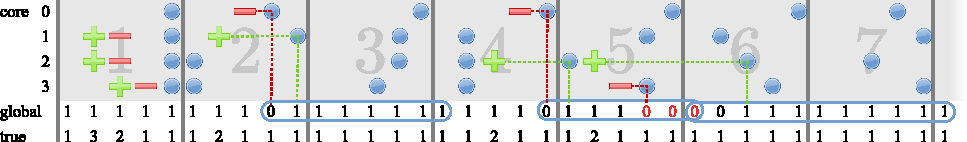
\includegraphics[width=\textwidth]{figures/refcache.pdf}
  \caption{\refcache example showing a single object over eight
    epochs.  Plus and minus symbols represent increment and decrement
    operations, dotted lines show when cores flush these to the object's
    global count, and blue circles show when each core flushes its
    local reference cache.  The loops around the global count show
    when the object is in core 0's review queue and
    the red zeroes indicate dirty zeroes.}
  \label{fig:refcache-ex}
\end{figure*}

\Cref{fig:refcache-ex} gives an example of a single object over
the course of eight epochs.  Epoch 1 demonstrates the power of
batching: despite six reference count manipulations spread over three
cores, the object's global reference count is never written to and
cache line conflicts arise only from epoch maintenance.  The
remaining epochs demonstrate the complications that arise from
batching and the resulting lag between the true reference count and
the global reference count of an object.

Because of the flush order, the two updates in epoch 2 are applied to
the global reference count in the opposite order of how they actually
occurred.  As a result, core 0 observes the global count temporarily
drop to zero when it flushes in epoch 2, even though the true count is
non-zero.  This is remedied as soon as core 1 flushes its increment,
and when core 0 reexamines the object at the beginning of epoch 4,
after all cores have again flushed their delta caches, it can see
that the global count is non-zero; hence, the zero count it observed
was not a true zero and the object should not be freed.

It is necessary but not sufficient for the global reference count to
be zero when an object is reexamined; there must also have been no
deltas flushed to the object's global count in the interim, even if
those changes canceled out or the deltas themselves were zero.
%
For example, core 0 will observe a zero global reference count
at the end of epoch 4, and again when it reexamines the object in
epoch 6.  However, the true count is not zero, and the global
reference count was temporarily non-zero during the epoch.  We call
this a \emph{dirty} zero and in this situation \refcache will
queue the object to be examined again two epochs later, in epoch 8.

\subsubsection{Weak references}
As described, \refcache is well suited to reference counts that track
the number of true references to an object, since there is no danger
of the count going back up from zero once the object becomes unreachable.
However, operating systems often need untracked references to objects;
for example, \fs's caches track objects that may be deleted at any time,
and may even need to bring an object's reference count back up from
zero.  \vm's radix tree has similar requirements.  To support such
uses, we extend \refcache with \emph{weak references}, which provide a
\code{tryget} operation that will either increment the object's
reference count (even if it has reached zero) and return the object,
or will indicate that the object has already been deleted.

A weak reference is simply a pointer marked with a ``dying'' bit,
along with a back-reference from the referenced object.  When an
object's global reference count initially reaches zero, \refcache sets
the weak reference's dying bit.  After this, \code{tryget} can
``revive'' the object by atomically clearing the dying bit and
fetching the pointer value, and then incrementing the object's
reference count as usual.  When \refcache decides to free an object,
it first atomically clears both the dying bit and the pointer in the
weak reference.  If this succeeds, it can safely delete the object.
If this fails, it reexamines the object again two epochs later.  In a
race between \code{tryget} and deletion, which operation succeeds is determined
by which clears the dying bit first.

This protocol can be extended to support multiple weak references per
object using a two phase approach in which all weak references are
first put in an intermediate state that can be rolled back if any
reference turns out to be revived.  Our current implementation does
not support this because it was not necessary for \vm or \fs.

\subsubsection{Algorithm}
\Cref{fig:refcache-code} gives pseudocode for \refcache.  Each core
maintains a hash table
storing its reference delta cache and the review queue that tracks
objects whose global reference counts reached zero.  A core reviews an
object after two epoch boundaries have passed, which guarantees
that all cores have flushed their
reference caches at least once.

\XXX![AC]{Make pseudo-code formatting consistent with rule chapter.}

\begin{figure}
  \def\fgap{-0.25em}            % Fit on a page
  \begin{tabbing}
    \quad\=\quad\=\quad\=\quad\=\quad\=\quad\=\kill
    inc(obj): \+\\
      if local cache[hash(obj)].obj $\ne$ obj: \+\\
        evict(local cache[hash(obj)]) \\
        local cache[hash(obj)] $\gets$ $\langle$obj, 0$\rangle$ \-\\
      local cache[hash(obj)].delta += 1 \\
    \-\\[\fgap]
    tryget(weakref): \+\\
      do: \+\\
        $\langle$obj, dying$\rangle$ $\gets$ weakref \-\\
      while weakref.cmpxchng($\langle$obj, dying$\rangle$,
        $\langle$obj, false$\rangle$) fails \\
      if obj is not null: \+\\
        inc(obj) \-\\
      return obj \\
    \-\\[\fgap]
    evict(obj, delta): \+\\
      % If this condition is true, then the locked region would be a
      % no-op, but why is it safe to do it without the lock?  The
      % danger is that the read of refcnt will slip in the middle of
      % another region that modified refcnt with obj locked.  evict
      % is the only place this happens and it does only a single write
      % to refcnt.  Assuming both this read and that write are
      % atomic, then we can consider this check atomic with the entire
      % locked region in the competing evict.
      if delta = 0 and obj.refcnt $\ne$ 0: return \\
      with obj locked: \+\\
        obj.refcnt $\gets$ obj.refcnt + delta \\
        if obj.refcnt = 0: \+\\
          if obj is not on any review queue: \+\\
            obj.dirty $\gets$ false \\
            obj.weakref.dying $\gets$ true \\
            add $\langle$obj, epoch$\rangle$ to the local review
            queue \-\\
          else: \+\\
            obj.dirty $\gets$ true \\
    \-\-\-\-\\[\fgap]
    flush(): \+\\
      evict all local cache entries and clear cache \\
      update the current epoch \\
    \-\\[\fgap]
    review(): \+\\
      flush() \\
      for each $\langle$obj, objepoch$\rangle$ in local review queue: \+\\
        if epoch $<$ objepoch + 2: continue \\
        with obj locked: \+\\
          remove obj from the review queue \\
          if obj.refcnt $\ne$ 0: \+\\
            obj.weakref.dying $\gets$ false \-\\
          else if obj.dirty or obj.weakref.cmpxchng(%
                $\langle$obj, true$\rangle$,
                $\langle$null, false$\rangle$) fails: \+\\
            obj.dirty $\gets$ false \\
            obj.weakref.dying $\gets$ true \\
            add $\langle$obj, epoch$\rangle$ to the local review queue \-\\
          else: \+\\
            free obj
  \end{tabbing}
  \vspace{-1em}                 % No idea where this space comes from
  \rule{\columnwidth}{0.5pt}
  \vspace{-\baselineskip}
  \caption[\refcache algorithm.]
  {\refcache algorithm.  Each core calls \code{review}
    periodically.  \code{evict} may be called by \code{flush} or because of a
    collision in the reference cache.  \code{dec} is identical to \code{inc} except
    that it decrements the locally cached delta.}
  \label{fig:refcache-code}
\end{figure}

All of the functions in \cref{fig:refcache-code} execute with
preemption disabled, meaning they are atomic with respect to each
other on a given core, which protects the consistency of per-core data
structures.  Fine-grained locks protect the \refcache-related fields
of individual objects.

For epoch management, our current implementation uses a barrier scheme
that tracks a global epoch counter, per-core epochs, and a count of
how many per-core epochs have reached the current global epoch.  This
scheme suffices for our benchmarks, but schemes with fewer cache-line
conflicts are
possible, such as the tree-based quiescent state detection used
by Linux's hierarchical RCU implementation~\cite{lwn:treercu}.

\subsubsection{Discussion}
\refcache trades latency for scalability by batching increment and
decrement operations in per-core caches.  As a result, except when
collisions in the reference delta cache cause evictions, \code{inc}
and \code{dec} are naturally conflict-free with all other operations.
%
Furthermore, because \refcache uses per-core caches
rather than per-core counts, it is more space-efficient than other
scalable reference counting techniques.  While not all uses of
reference counting can tolerate \refcache's latency, its scalability
and space-efficiency are well suited to the requirements of \vm and
\fs.

\XXX[Austin]{Design alternatives: token-passing or broadcast IPI for
epoch detection; lock-free versus fine-grained locking?}


\subsection{RadixVM: Scalable address space operations}

\XXX[AC]{``Disjoint'' instead of ``non-overlapping''?  Should at least
be consistent.}

The POSIX virtual memory interface is rife with commutativity, but
existing implementations scale poorly.  We model a virtual memory
system as four key logical operations: \code{mmap} adds a region of
memory to a process' virtual address space, \code{munmap} removes a
region of memory from the address space, and \code{memread} and
\code{memwrite} access virtual memory at a particular virtual address
or fail if no mapped region contains that address.  In reality, the
hardware implements \code{memread} and \code{memwrite} directly and
the VM system instead implements a \code{pagefault} operation; we
discuss this distinction below.

% Old, implementation-oriented text:
% A typical virtual memory system supports three key operations:
% \code{mmap} to add a region of memory to a process's virtual memory
% address space, \code{munmap} to remove a region of memory from the
% address space and the corresponding pages from the hardware page
% tables, and \code{pagefault}, which inserts a page into the hardware
% page tables at the faulting virtual address, allocating a new physical
% page if necessary.

% Old, more detailed memread/memwrite text:
% In reality, the hardware implements \code{memread} and \code{memwrite}
% directly using a cache of virtual-to-physical translations; when an
% operation misses in this translation cache, the hardware invokes
% \code{pagefault}, which is provided by the VM system.  This
% translation cache does not affect the interface specification or its
% commutativity; we'll discuss its effect on implementation below.

VM operations from \emph{different} processes (and hence address
spaces) trivially commute.  Most existing implementations use
per-process address space representations, so such operations are also
naturally conflict-free (and scale well).  VM operations from the same
process also often commute; in particular, operations on
\emph{non-overlapping} regions of the address space commute.
%
Many multithreaded applications exercise exactly this increasingly
important scenario: \code{mmap}, \code{munmap}, and related variants
lie at the core of high-performance memory allocators and garbage
collectors and partitioning the address space between threads is a key
design component of these
systems~\cite{ssmalloc:apsys,jemalloc,tcmalloc}.  Applications that
frequently map and unmap files also generate such workloads for the OS
kernel.

Unfortunately, owing to complex invariants in virtual memory systems,
widely used kernels such as Linux and FreeBSD protect each address
space with a single lock.  This induces not only conflicts but, often,
complete serialization between commutative VM operations on the same
address space, which can dramatically limit application
scalability~\cite{boyd-wickizer:scaling,clements:bonsai}.
\XXX{Mention workarounds or at least add that tidbit from Google?}

\vm is a novel virtual memory system in which commutative operations
on non-overlapping address space regions are almost always
conflict-free.  This ensures that if two threads operate on distinct
regions of virtual memory, the VM system does not limit the
application's scalability.  Furthermore, if multiple threads operate
on the same shared region, \vm constrains conflicts to the cores
executing those threads.

Achieving this within the constraints of virtual memory hardware,
without violating POSIX's strict requirements on the ordering and
global visibility of VM operations, and without unacceptable memory
overhead is challenging.  The following sections describe \vm's
approach.  \Cref{sec:radixvm:arch} describes the general architecture
of POSIX VM systems.  \Cref{sec:radixvm:tree,sec:radixvm:tlb} describe
the data structures that form the core of \vm.  Finally,
\cref{sec:radixvm:ops} describes how \vm uses these structures to
implement standard VM operations.


\XXX[AC]{Not sure where to say the following, but I think we need to
  be clear that none of these subsystems 100\% follows the rule, but
  that that's okay from an engineering standpoint:

  Like \refcache, \vm sacrifices strict adherence to the scalable
  commutativity rule in the interest of practical constraints on
  memory consumption and sequential performance.  Complex software
  systems inevitably involve conflicting requirements and scalability
  is no different.  However, in designing \vm, the presence of the
  rule forced us to explicitly recognize, evaluate, and justify where
  we made such trade-offs.}

\XXX![AC]{This uses subsubsections, but \refcache uses paragraphs.}

\XXX![AC]{Copy in some related work section bits from EuroSys.}

\subsubsection{POSIX VM architecture}
\label{sec:radixvm:arch}

\begin{figure}
  \centering
  \XXX!{Mapped regions, page tables, TLB with application on top.  See
    Bonsai Figure 1 and \vm talk.}
  \caption[Key structures in a POSIX VM system.]{Key structures in a
    POSIX VM system, showing an address space with four mapped
    regions.  Crossed-out page table entries are marked ``not
    present.''  Some pages have not been faulted yet, and thus are not
    present, despite being in a mapped region.}
  \label{fig:vm-structures}
\end{figure}

Between the POSIX VM interface on one side and the hardware virtual
memory interface on the other, \vm's general architecture necessarily
resembles typical Unix VM systems.  \Cref{fig:vm-structures} shows the
principle structures any Unix VM system must manage.  On the left is
the kernel's internal representation of the address space.  Logically,
this consists of a set of mapped regions of the virtual address space,
where each region may map either a file or ``anonymous'' (heap)
memory, has various access permissions, and may be either shared
across \code{fork} or copied.  \code{mmap} and \code{munmap} directly
manipulate this view of the address space.

However, translating virtual addresses to physical addresses is
ultimately performed in hardware---specifically by the memory
management unit (MMU)---and the MMU's representation of virtual memory
generally differs significantly from the kernel's internal
representation of the address space.  Most hardware architectures
specify some form of page table, like the x86 page table depicted in
\cref{fig:vm-structures}, for the kernel to inform the MMU of the
mapping from virtual addresses to physical addresses.  These
structures map addresses at a page granularity (typically 4~KB, though
most architectures also support larger pages) and represent access
permissions (which are checked by the MMU), but have little
flexibility.

While we model the VM system in terms of \code{mmap}, \code{munmap},
\code{memread}, and \code{memwrite}, only the first two are directly
implemented by the VM system.  The latter two are implemented by the
MMU using the kernel-provided page table.  However, the VM system has
a key hook into the MMU: when the virtual address of a read or a write
is marked ``not present'' in the page table or fails a permission
check, the MMU invokes the VM system's \code{pagefault} operation.
Modern Unix kernels exploit this mechanism to implement \emph{demand
  paging}, populating page table entries by allocating pages or
reading them from disk only once a page is first accessed, rather than
when it is mapped.
%
Hence, \code{mmap} and \code{munmap} simply clear the page table
entries of the region being mapped or unmapped; \code{mmap} depends on
\code{pagefault} operations to later fill these entries with mappings.
%
While demand paging significantly affects the implementation of the VM
system, it is nevertheless an implementation issue and does not affect
the commutativity of \code{memread} or \code{memwrite}.

The final key structure the VM system must manage is the hardware
translation lookaside buffer (TLB).  The TLB is a per-core associative
cache of virtual-to-physical mappings.  In architectures with a
hardware-filled TLB (x86, ARM, PowerPC, and many others), the MMU
transparently fills this cache from the page table.  Invalidating the
TLB, however, is the responsibility of the VM system.  Hence,
\code{munmap}, in addition to removing regions from the kernel's
internal address space representation and clearing entries in the page
table, must also invalidate the corresponding TLB entries.


\subsubsection{Radix tree}
\label{sec:radixvm:tree}

% At its core, an address space is a mapping from virtual addresses to
% physical addresses and metadata.  Hence, \vm needs a data structure
% that can track this mapping and support \code{mmap}ing and
% \code{munmap}ing ranges of virtual address space while avoiding
% conflicts between operations on disjoint regions.

We first tackle \vm's internal address space representation.
%
Widely-used operating system kernels represent an address space as a
balanced tree of mapped memory regions.  For example, Linux uses a
red-black tree~\cite{linux-source}, FreeBSD uses a splay
tree~\cite{freebsd-source}, and Solaris and Windows use AVL
trees~\cite{windows:wrk,windows:slides}).  This ensures fast lookups
and modifications for address spaces that can easily contain thousands
of mapped regions, but these data structures are poorly suited for
concurrent access: not only do they induce cache line conflicts
between operations on disjoint regions, they force all of these
kernels to use coarse-grained locking.

Lock-free data structures seem like a compelling solution to this
problem.  However, while lock-free data structures such as the Bonsai
tree used by the Bonsai VM~\cite{clements:bonsai} and lock-free skip
lists~\cite{herlihy:art} eliminate the coarse-grained serialization
that plagues popular VM systems, their operations are far from
conflict-free.  For example, \code{insert} and \code{lookup}
operations for a lock-free concurrent skip list can conflict on
interior nodes in the skip list---even when the \code{lookup} and
\code{insert} involve different keys and hence commute---because
\code{insert} must modify interior nodes to maintain $O(\log n)$
lookup time.  Indeed, any balanced data structure will suffer from
such problems.

A (completely impractical) way to achieve conflict-free commutative
operations is to represent a process's address space by storing the
metadata for each
virtual page individually in a large linear array indexed by virtual
page number.  In this linear representation, \code{mmap}, \code{munmap},
and \code{pagefault} can lock and manipulate precisely the pages being
mapped, unmapped, or faulted and operations on non-overlapping regions
are clearly conflict-free.  The design of \vm follows the same general
scheme as this strawman design, but reins in its memory consumption
using a multilevel, compressed radix tree.

\begin{figure}
\centering
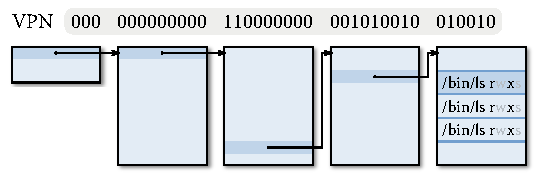
\includegraphics{figures/radix.pdf}
\caption{A radix tree containing both an anonymous mapping
  and a file mapping.  Blue indicates the path for looking up the 36-bit
  virtual page number shown in bits at the top of the figure.  The last
  level of the tree contains separate mapping metadata for each page.
}
\label{fig:radix}
\end{figure}

The index data structure of \vm resembles a hardware page table
structurally, storing mapping metadata in a fixed-depth radix tree,
where each level of the tree is indexed by nine (or fewer) bits of the
virtual page number (\cref{fig:radix}).  Like the linear array,
the radix tree supports only point queries (not range queries) and
iteration, but unlike the linear array, \vm can compress repeated
entries and lazily allocate the nodes of the radix tree.  Logically,
any node that would consist entirely of identical values is folded
into a single value stored in the parent node.  This continues up to
the root node of the tree, allowing the radix tree to represent vast
swaths of unused virtual address space with a handful of empty slots
and to set large ranges to identical values very quickly.  This
folding comes at a small cost: operations that expand a subtree will
conflict with other operations in that same subtree, even if their
regions do not ultimately overlap.  However, after initial address
space construction, the radix tree is largely ``fleshed out'' and
these initialization conflicts becomd rare.

To record each mapping, \vm stores a separate copy of the mapping metadata
in the radix tree for each page in the mapped range.  This differs
from a typical design that allocates a single metadata object
to represent the entire range of a mapping (e.g., ``virtual memory
areas'' in Linux).
%
This is practical because \vm's mapping metadata object is small and
designed so that it will initially be byte-wise
identical for every page of a mapping, meaning that large mappings can
created efficiently and folded into just a few slots in the radix
tree's nodes.

Also unlike typical virtual memory system designs, \vm stores pointers
to physical memory pages in the mapping metadata for pages that have
been allocated.  This is easy to do in \vm because, modulo folding,
there is a single mapping metadata object for each page.  It's also
important to have this canonical representation of the physical memory
backing a virtual address space because of the way \vm handles TLB
shootdown (see \cref{sec:radixvm:tlb}).  This does increase the space
required by the radix tree, but, asymptotically, it's no worse than
the hardware page tables, and it means that the hardware page tables
themselves are cacheable memory that can be discarded by the OS to
free memory.

To keep the memory footprint of the radix tree in check, the OS must be
able to free nodes that no longer contain any valid mapping metadata.
To accomplish this without introducing undue conflicts, we leverage
\refcache to scalably track the number of used slots in each node.
When this count drops to zero, the radix tree can remove the node from
the tree and delete it.  Since \vm may begin using a node again before
\refcache reconciles the used slot count, nodes link to their children
using weak references, which allows the radix tree to revive nodes
that go from empty to used before \refcache deletes them, and to
safely detect when an empty child node has been deleted.

Collapsing the radix tree does potentially introduce conflicts;
however, unlike with eager garbage collection schemes, rapidly
changing
mappings cannot cause the radix tree to rapidly delete and recreate
nodes.  Since a node must go unused for at least two \refcache epochs
before it is deleted, any cost of deleting or recreating it (and any
additional contention that results) is amortized.
\XXX[AC]{We don't actually implement this, but if we did, when we
analyze performance without \refcache, things would be even worse.
Might be worth mentioning.}

In contrast with more traditional balanced trees, using a radix tree
to manage address space metadata allows \vm to achieve near-perfect
conflict-freedom (and hence scalability) for metadata operations on
non-overlapping regions of an address
space.  This comes at the cost of a potentially larger memory
overhead; however, address space layouts tend to exhibit good
locality and folding efficiently compresses large ranges, making radix
trees a good fit for a VM system.
\XXX[AC]{We show this in the \vm paper.  Pull that in here or in the
  evaluation?}

\subsubsection{TLB management}
\label{sec:radixvm:tlb}

The other major impediment to scaling \code{mmap} and \code{munmap}
operations is the need to explicitly invalidate cached
virtual-to-physical mappings in per-core TLBs when a page is unmapped
(or remapped).
%
Because TLB shootdowns must be performed on every CPU that may have
cached a page mapping that's being modified, and because hardware does
not provide
information about which CPUs may have cached a particular mapping,
typical Unix VM systems send TLB shootdown interrupts to all
CPUs using the modified address space, inducing cache line conflicts
and limiting scalability.

\vm addresses this problem by precisely tracking the set of CPUs that
have accessed each page mapping.
%
In architectures with software-filled TLBs (such as the MIPS or
UltraSPARC) this is easy, since the MMU informs the kernel of each
miss in the TLB.  The kernel can use these TLB miss faults to track
exactly which CPUs have a given mapping cached and, when a later
\code{mmap} or \code{munmap} changes this mapping, it can deliver
shootdown requests
only to cores that have accessed this mapping.  On architectures
with hardware-filled TLBs such as the x86, \vm achieves the
same effect using per-core page tables.
%
With TLB tracking, if an application thread
allocates, accesses, and frees memory on one core, with no other threads
accessing the same memory region, then \vm will perform no TLB shootdowns.

The obvious downside to this approach is the extra memory required for
per-core page tables.  We show in \cref{eval:memory} that this
overhead is small in practice compared to the total memory footprint
of an application, but for applications with poor partitioning, it may
be necessary for the application to provide hints about widely shared
regions so the kernel can share page tables (similar to Corey address
ranges~\cite{boyd-wickizer:corey}) or for the kernel to detect such
regions.
%
\XXX![AC]{Do we show this in \cref{eval:memory}?}
%
The kernel could also reduce overhead by simply discarding page table
pages when memory is low.

\subsubsection{VM operations}
\label{sec:radixvm:ops}

With the components described above, \vm's implementation of the core
VM operations is surprisingly straightforward.
%
One of the most difficult aspects of the POSIX VM interface in a
multicore setting is its strict ordering and global visibility
requirements~\cite{clements:bonsai}.  For example, after the return
of an \code{munmap}, no thread on any core should be able to access
the unmapped
region.  Similarly, after \code{mmap} returns, any thread on any core
must be able to access the mapped region.  Furthermore, though not
required by POSIX, it is generally assumed that these operations are
atomic.

\vm enforces these semantics by always locking, from left to right,
the bottom-most radix tree entries for the region of an operation.
This simple mechanism ensures all operations on an address space are
linearizable~\cite{herlihy:linearizability} and, for fully expanded
subtrees, prevents cache line conflicts between operations on disjoint
regions.

% When locking a region that has not been expanded out to leaf nodes
% yet, \vm acquires locks on the corresponding internal node slots
% instead.  When \vm expands the tree by allocating new nodes, it
% propagates the lock bit to every entry in the newly allocated node,
% and unlocks the parent interior node slot.  Releasing the lock
% clears the lock bits in the newly allocated child node.  Tree
% traversal does not require locks or indeuce conflicts because it
% increments each node's reference count through a \refcache weak
% reference.

An \code{mmap} invocation, like all \vm operations, first locks the
range being mapped.
%
If there are existing mappings within the
range, \code{mmap} unmaps them, as described later for \code{munmap}.
\code{mmap} then fills in mapping metadata for the new mapping (protection
level and flags arguments to \code{mmap}, as well as what backs this virtual
memory range, such as a file or anonymous memory).  If the mapping covers
an entire radix tree node, and the child nodes have not been allocated
yet, the radix tree collapses the mapping metadata into a single slot
in the interior of the tree.
Otherwise, \vm copies the mapping metadata into each leaf node entry in
the range.  Finally, \vm unlocks the range.  Like in other VM systems,
\code{mmap}
doesn't allocate any physical pages, but leaves that to \code{pagefault},
so that pages are allocated only when they are used.

A \code{pagefault} invocation traverses the radix tree to find the
mapping metadata for the faulting address, and acquires a lock on it.
It then allocates a physical page if one has not been allocated yet
(for anonymous memory), or fetches it from the buffer cache (for file
mappings) and
stores it in the mapping metadata.  Finally, \code{pagefault} fills in the
page table entry in the local core's page table, and adds the local core
number to the TLB shootdown list in the mapping metadata for that address.
\code{pagefault} then releases the lock and returns.

To implement \code{munmap}, \vm must clear mapping metadata from the
radix tree, clear page tables, invalidate TLBs, and free physical
pages.  \code{munmap} begins by locking the range being unmapped,
after which it can scan the region's metadata to gather references to
the physical pages backing the region, collect the set of cores that
have faulted pages in the region into their per-core page tables, and
clear each page's metadata.  It can then send inter-processor
interrupts to the set of cores it collected in the first step.  These
interrupts cause the remote cores (and the core running \code{munmap})
to clear the appropriate range in their per-core page table and
invalidate the corresponding local TLB entries.  Once all cores have
completed this shootdown process, \code{munmap} can safely release its
lock on the range and decrement the reference counts on the physical
pages that were unmapped.

Note that an invocation of \code{pagefault} on one core may concurrently
access a page that another core is in the process of unmapping,
but the mapping metadata lock makes this work out correctly: either
\code{pagefault} acquires the lock first or \code{munmap} does.  In the
first case, the page fault succeeds, which is okay since the pages must be
inaccessible only after \code{munmap} returns.  In the second case,
\code{munmap} runs first and removes the mapping for the unmapped range
before releasing the locks. Then, \code{pagefault} will see that there
is no mapping for the faulting address and will halt the faulting thread.

\subsubsection{Discussion}

By combining \refcache for scalable reference counting, radix trees
for maintaining address space metadata, and per-core page tables for
precise TLB tracking and shootdown, \vm achieves conflict-freedom for
the vast majority of commutative VM operations.  The clear
commutativity properties of the POSIX VM interface, combined with the
right data structures makes this possible with a straightforward
concurrency plan based on precise range locking.
%
As shown in \cref{fig:testcase-breakdown-sv6}, \tool confirmed that
most commutative operations in \vm are conflict-free.  In
\cref{sec:eval}, we further confirm that \vm's design translates into
scalable performance for application workloads. \XXX![AC]{Do we
  confirm this?}


\subsection{\fs: Conflict-free file system operations}

\XXX[FK/AC]{Make this more like \vm section.  Lead with operations and
  their rough commutativity.  Since the high-level structure is much
  more like a conventional VFS than \vm is like a convention VM, say
  that and then explain some key detail (probably something involving
  hash tables).  E.g., how the inode cache works.  (See FK edits for
  init-154-6dbae76)}

\fs encompasses \sys's unified buffer cache and VFS layers, providing
operations such as \code{read}, \code{write}, \code{open}, and
\code{unlink}.  We focused on the VFS and buffer cache layers because
these are the common denominators of all file systems in a Unix
kernel.
%
In contrast with \vm,
\fs makes extensive use of well-known techniques for scalable
implementations, such as per-core resource
allocation, double-checked locking, lock-free readers using
RCU~\cite{rcu:linux},
and seqlocks~\cite[\S6]{lameter:linuxsync}.
%
\fs also employs \refcache for tracking both internal resources and
inode link counts.
%
\fs is also structured much like contemporary Unix VFS subsystems,
with inode and directory caches represented as concurrent hash tables
and per-file page caches.
%
What sets \fs apart is that the details of its implementation were
guided by the scalable commutativity rule and, in particular, by
\tool.
%
This led to several common design patterns, which we illustrate with
example test cases from \tool{}:
%
\XXX[AC]{\fs is more irregular than \vm, so \tool was more important.}


\paragraph{Layer scalability.}  \fs uses data structures that
themselves naturally satisfy the commutativity rule, such as linear
arrays, radix trees, and hash tables.  In
contrast with structures like balanced trees, these data
structures
typically share no cache lines when different elements are accessed
or modified.  For example, \fs stores the cached data pages for a given inode
using a radix tree, so that concurrent reads or writes to different
file pages scale, even in the presence of operations
extending or truncating the file.
% , as long as they don't access the part
% of the file that's being extended or truncated.
\tool led us to an additional benefit of this representation:
many operations also use this radix tree to determine if some offset
is within the file's bounds without reading the size and conflicting
with operations
that change the file's size.
%
For example, \code{pread} first probes this radix tree for the
requested read offset: if the offset is beyond the last page of the
file, it can return 0 immediately without reading (and potentially
conflicting on) the file size.

\XXX[FK]{``Defer work'' can be presented as dealing with
  non-commutative ops.}

\paragraph{Defer work.} Many \fs resources are shared,
such as file descriptions and inode objects, and must be freed when no
longer referenced.
Typically, kernels release resources immediately, but this requires
eagerly tracking references to resources, causing
commutative operations that access the same resource to conflict.  Where
releasing a resource is not time-sensitive, \fs
uses Refcache to batch reference count
reconciliation and zero detection.  This way, resources are eventually
released, but within each Refcache epoch commutative operations can be
conflict-free.

\XXX[AC]{Discuss crazy pipe hybrid reference counting scheme?}

Some resources are artificially scarce, such as inode numbers in a typical
Unix file system.  When a typical Unix file system runs out of free
inodes, it must reuse an inode from a recently deleted file.
%
This requires finding and garbage collecting unused inodes, which
induces conflicts.
%
However,
the POSIX interface does not require that inode numbers be reused, only
that the same inode number is not used for two files at once.  Thus,
\fs never reuses inode numbers.  Instead, inode numbers are
generated by a monotonically increasing per-core counter, concatenated
with the core number that allocated the inode.  This allows \fs to defer
inode garbage collection for longer periods of time, and enables
conflict-free and scalable
per-core inode allocation.


% \paragraph{Check before updating.}  Before updating any data structure,
% \fs first checks whether the data structure already contains the new
% value, and avoid any writes if so.  For example, the Linux file system
% always acquires a lock on an inode when truncating the file.  This means
% that concurrent truncate operations do not scale, even if the file
% is already empty.  \fs first checks the current length of the file,
% and avoids updating the length or acquiring any locks if the file is
% already at the right size.

% As another example, if one thread tries to create an existing file using
% \code{open(O_CREAT|O_EXCL)}, it should fail, but a na\"ive implementation
% might first acquire a lock to prepare for creating the file, and then
% check whether the file already exists.  This makes
% concurrent \code{open(O_CREAT|O_EXCL)} calls for an existing file name
% non-scalable.  \fs first checks whether the file already exists without
% modifying any cache lines, making these operations scale.

% \XXX[AC]{The above two examples are slightly off.  E.g., if I do two
% truncates and the first writes to the file length and the second reads
% that, that's sharing.  These are both idempotent updates, which is one
% of the few things we \emph{don't} do scalably.}

% As a final example, if two file names \code{a} and \code{b} point to the
% same inode, \code{rename(a, b)} should remove the directory entry for
% \code{a}, but it should not modify the directory entry for \code{b}, since
% it already points at the right inode.  By checking the directory
% entry for \code{b} before updating it, \fs allows \code{rename(a, b)}
% to scale with other operations that look up \code{b}.


\paragraph{Precede pessimism with optimism.} Many operations
in \fs have an optimistic check stage followed by a pessimistic update
stage, a generalized sort of double-checked locking.  The optimistic
stage checks conditions for the operation and returns immediately if
no updates are necessary (this is often the case for error returns,
but can also happen for success returns).  This stage does no writes
or locking, but because no updates are necessary, it is often easy to
make atomic.  If updates are necessary, the operation acquires
locks or uses lock-free protocols, re-verifies its conditions to
ensure atomicity of the update stage, and performs updates.  For
example, \code{lseek} first computes the new offset using a lock-free
read-only protocol and returns early if the new offset is invalid or
equal to the current offset.  Otherwise, \code{lseek} locks the file
offset and re-computes the new offset to ensure consistency.
%
In fact, \code{lseek} has surprisingly complex interactions with
system state and other operations, and arriving at a protocol that was
both correct and conflict-free in all commutative cases would have
been difficult without \tool.

\code{rename} is similar.  If two file names \code{a} and \code{b}
point to the
same inode, \code{rename(a, b)} should remove the directory entry for
\code{a}, but it does not need to modify the directory entry for
\code{b}, since
it already points at the right inode.  By checking the directory
entry for \code{b} before updating it, \code{rename(a, b)} avoids
conflicts with other operations that look up \code{b}.
%
As we saw in \cref{sec:topic:rename-conditions}, \code{rename} has
many surprising and subtle commutative cases and, much like
\code{lseek}, \tool was instrumental in helping us arrive at an
implementation that was conflict-free in these cases.


\paragraph{Don't read unless necessary.}  A common internal interface
in a file system implementation is a \code{namei} function that
checks whether a path name exists, and if so, returns the inode for
that path.
%
However, reading the inode is unnecessary
if the caller wants to know only whether a path name existed, such as
an \code{access(F_OK)} system call.  In particular, the \code{namei}
interface makes it impossible for concurrent \code{access(b, F_OK)}
and \code{rename(a, b)} operations to scale when \code{a} and \code{b}
point to different inodes, even though they commute.
\fs has a separate internal interface to check for existence of a
file name, without looking up the inode, which allows \code{access}
and \code{rename} to scale in such situations.


\subsection{Difficult-to-scale cases}

As \cref{fig:testcase-breakdown-sv6} illustrates, there are a few
(\pyexpr{mscan.xv6.shared} out of \pyexpr{mscan.ntestcases})
commutative test cases for
which \vm and \fs are not conflict-free.
%
The majority of these tests involve idempotent updates to internal
state, such as two \code{lseek} operations that both seek a file
descriptor to the same offset, or two anonymous \code{mmap} operations
with the same fixed base address and permissions.  While it is
possible implement these scalably, every implementation we considered
significantly impacted the performance of more common operations, so
we explicitly chose to favor common-case performance over total
scalability.  Even though we decided to forego scalability in these
cases, the commutativity rule and \tool forced us to consciously make
this trade-off.
%
\XXX[AC]{About 75\% are known idempotent.}

% Non-idempotent shared case list (incomplete):
% close_close_pe_5: Closing pipe writer (eager counting)
% close_read_pdc_0: Closing pipe writer, reading writer always EBADF
% close_write_pd8_0: Symmetric to close_read_pdc_0
% lseek_read_pad8_2: Reading nothing from two different offsets
% lseek_read_p8b6_3: Same as lseek_read_pad8_2
% mmap_mprotect_pf8_41: Making different read-only mappings read-only
%   (The mprotect is a no-op, but what it reads is modified)
% mmap_mprotect_pae_40: Same
% read_read_pce4_0: Two reads from a file full of zeroes
% read_write_pbb0_2: Reading nothing from different end-of-file offsets
% write_write_pff8_1: Writing to a pipe with no readers
%   (We could probably fix this one)
% write_write_pff8_2: Same
% write_write_pf78_1: Same

Other difficult-to-scale cases are more varied.  Several involve
reference counting of pipe file descriptors.  Closing the last file
descriptor for one end of a pipe must immediately affect the other
end; however, since there's generally no way to know a priori if a
\code{close} will close the pipe, a shared reference count is used in
some situations.  Other cases involve operations that return the same
result in either order, but for different reasons, such as two reads
from a file filled with identical bytes.
%
By the rule, each of these cases has some conflict-free
implementation, but making these particular cases conflict-free would
have required sacrificing the conflict-freedom of many other
operations.


\XXX[AC]{fstest works around all radix tree expansion.  Is this
cheating?  That's actually an interesting case.}

\XXX[AC]{Summarize or something?}

\section{Performance evaluation}
\label{sec:eval}

\XXX[STATUS]{Draft v2 ready.  Merged SOSP and \vm evaluations.
  New(ish) intro and discussion sections.  Applied Frans' edits from
  init-228-g69596c0, except for moving more implementation-related
  content to previous chapter.}

Given that nearly all commutative \fs and \vm operations are
conflict-free, in principle, applications built on these operations
should scale perfectly.
%
\Thiscref{sec:eval} confirms this, completing a pyramid whose
foundations were set in \cref{sec:scalability} when we demonstrated
that conflict-free memory accesses scale in most circumstances on real
hardware.
%
\Thiscref{sec:eval} extends these results, showing that complex
operating system calls built on conflict-free memory accesses scale
and that, in turn, applications built on these operations scale.
%
We focus on the following questions:

\begin{CompactItemize}

\item Do conflict-free implementations of commutative operations and
  applications built using them scale on real hardware?

\item Do non-commutative operations limit performance on real
  hardware?

% \item Does optimizing for scalability sacrifice sequential performance?

\end{CompactItemize}

Since real systems cannot focus on scalability to the exclusion of
other performance characteristics, we also consider the balance of
performance requirements by exploring the following question:

\begin{CompactItemize}

\item Can implementations optimized for linear scalability of
  commutative operations also achieve competitive sequential
  performance, reasonable (albeit sub-linear) scalability of
  non-commutative operations, and acceptable memory use?

\end{CompactItemize}


To answer these questions, we use \sys.
In addition to the operations analyzed in \cref{sec:sv6}, we scalably
implemented
other commutative operations (e.g., \code{posix_spawn})
and many of the modified POSIX APIs from
\cref{sec:posix}.
%
All told, \sys
totals \pyexpr{const["xv6-loc"]["all"]} lines of code, including user
space and library code.
%
Using \sys, we evaluate two microbenchmarks and one application
benchmark focused on file system operations, and three microbenchmarks
and one application benchmark focused on virtual memory operations.


\subsection{Experimental setup}
\label{sec:topic:ben}


We ran experiments on an 80-core machine with eight 2.4~GHz 10-core
Intel E7-8870 chips and 256~GB of RAM (detailed earlier in
\cref{fig:machines}).
%
When varying the number of
cores, benchmarks enable whole sockets at a time, so each 30~MB
socket-level L3 cache is shared by exactly 10~enabled cores.
We also report single-core numbers for
comparison, though these are expected to be higher because without
competition from other cores in the socket, the one
core can use the entire 30~MB cache.

We run all benchmarks with the hardware prefetcher disabled because we
found that it often prefetched contended cache lines to cores that did
not ultimately access those cache lines, causing significant
variability in our benchmark results and hampering our efforts to
precisely control sharing.  We believe that, as large multicores and
highly parallel applications become more prevalent, prefetcher
heuristics will likewise evolve to not induce this false sharing.

As a performance baseline, we compare against the same
benchmarks running on Linux~3.5.7 from Ubuntu Quantal.
%
All benchmarks compile and run on Linux and \sys without modifications.
%
Direct comparison is difficult because
Linux implements many features \sys does not, but this comparison
confirms \sys's sequential performance is sensible.
% \XXX[AC]{Different version from mtrace, which is a little awkward.}
% %
% In the virtual memory benchmarks, we additionally compare against
% Linux with the Bonsai VM system~\cite{clements:bonsai} (based on
% kernel version 2.6.37).
% %
% Bonsai implements a \code{pagefault} operation that is usually
% conflict-free with commutative \code{pagefault}s, but still serializes
% \code{mmap} and \code{munmap} operations.

We run each benchmark three times and report the mean.  Variance from
the mean is always under 5\% and typically under 1\%.
% \XXX[AC]{Except mailbench with regular APIs on 80 cores, where
% something clearly went bonkers, and a few VM microbenchmark points
% on Linux and Bonsai, but they're so collapsed that mean variance
% doesn't mean much.}

\subsection{File system microbenchmarks}
\label{sec:eval:fs-microbenchmarks}

% Many interfaces provide stricter or more complex semantics than
% generally required by applications.  \code{fstat}, for example, combines
% several return values, including properties like a file's
% link count, while applications typically only need one or two of these
% properties, such as the file size or modification time.  Such interfaces
% often have limited commutativity, where slightly modified interfaces
% that better align with application needs may commute in more situations.
% \code{fstat} does not commute with \code{link} on the same inode because
% \code{link} modifies the link count that \code{fstat} returns, but if an
% application could request only, say, the file size, the resulting
% interface would commute with \code{link}.

% We call such cases, where operations do not commute according to the
% specification but weaker and more widely commutative semantics suffice
% for many applications, \emph{needless non-commutativity}.
% \XXX[AC]{Avoid ``needless non-commutativity.''  The point of the
% commutative versions of the benchmarks is just to verify that it's the
% non-commutativity limiting scalability.}

% In this section, we explore the impact of non-commutative interfaces on
% scalability by examining the scalability of some of the needlessly
% non-commutative POSIX interfaces discussed in
% \cref{sec:posix}. \XXX[FK]{I don't think we need this reference to
% section 6, and we could do without section 6, and turning it into a
% future work and discussion section.}

Each file system benchmark has
two variants, one that uses standard, non-commutative POSIX APIs and
another that accomplishes the same task using the modified, more broadly
commutative APIs from \cref{sec:posix}.
%
By benchmarking the standard interfaces against
their commutative counterparts, we can isolate the cost of
non-commutativity and also examine the scalability of
conflict-free implementations of commutative operations.

% We examine three different classes of
% non-commutativity: statbench exercises \code{fstat}, which combines
% several operations into one; openbench exercises file descriptor
% allocation, which has process-wide invariants; and sockbench exercises
% local sockets, which have strict ordering requirements.

\paragraph{\cmd{statbench}.} In general, it's difficult to argue that an
implementation of a
non-commutative interface achieves the best possible scalability for
that interface and that no implementation could scale better.  However,
in limited cases, we can do exactly this.  We start with \cmd{statbench},
which measures the scalability of \code{fstat} with respect to
\code{link}.  This benchmark creates a single file that $n/2$ cores
repeatedly \code{fstat}. The other $n/2$ cores repeatedly
\code{link} this file to a new, unique file name, and then \code{unlink}
the new file name.  As discussed in \cref{sec:posix}, \code{fstat} does not
commute with \code{link} or \code{unlink} on the same file because
\code{fstat} returns the link count.  In practice,
applications rarely invoke \code{fstat} to get the link count, so \sys
introduces \code{fstatx}, which allows applications to request specific
fields (a similar system call has been proposed for
Linux~\cite{linux:xstat}).

\XXX[AC]{Mention that commutative statbench helps verify our
disjoint-access parallelism assertion on real hardware.}

\newcounter{mysubfigure}[figure]
\renewcommand{\themysubfigure}{\thefigure(\alph{mysubfigure})}

\begin{figure*}
  \centering
  % Make subfigure labels refer to correct figure
  \stepcounter{figure}
  % Top-align the two graphs
  \tikzset{gnuplot/.append style={baseline=(current bounding box.north)}}
  \input{graph/linkbench.tex}
  \refstepcounter{mysubfigure}
  \label{fig:linkbench}
  \hspace{-.05in}
  \input{graph/fdbench.tex}
  \hspace{-0.2in}
  \refstepcounter{mysubfigure}
  \label{fig:fdbench}
  \addtocounter{figure}{-1}
  %
  \splitcaption{File system microbenchmark throughput}{in operations
    per second per core with
    varying core counts on \sys.
    The blue dots indicate single core Linux
    performance for comparison.}
\end{figure*}

% \begin{figure}
%   \centering
%   \input{graph/linkbench.tex}
%   \caption{\code{fstat} throughput with $n/2$ cores running \code{fstat}
%     and $n/2$ cores running \code{link}/\code{unlink}.}
%   \label{fig:linkbench}
% \end{figure}

We run \cmd{statbench} in two modes: one mode uses \code{fstat}, which does
not commute with the \code{link} and \code{unlink} operations performed
by the other threads, and the other mode uses \code{fstatx} to request
all fields except the link count, an operation that \emph{does} commute
with \code{link} and \code{unlink}.  We use a \refcache scalable
counter for the link count so that the
\code{link}s and \code{unlink}s are conflict-free, and place it on
its own cache line to avoid false sharing.
\Cref{fig:linkbench} shows the results.  With the commutative
\code{fstatx}, \cmd{statbench} scales perfectly for both \code{fstatx} and
\code{link}/\code{unlink} and experiences zero L2 cache
misses in \code{fstatx}.  On the other hand, the traditional
\code{fstat} scales poorly and the conflicts induced by \code{fstat}
impact the scalability of the threads performing \code{link} and
\code{unlink}.

%This is no implementation fluke. 
To better
isolate the difference between \code{fstat} and \code{fstatx}, we run
\cmd{statbench} in a
third mode that uses \code{fstat}, but represents the link count
using a simple shared counter instead of \refcache.  In this mode, \code{fstat}
performs better at low core counts, but \code{fstat}, \code{link}, and
\code{unlink} all suffer at higher core counts.
%
With a shared link count, each \code{fstat}
call experiences exactly one L2 cache miss (for the cache line
containing the link count), which means this is the most scalable that
\code{fstat} can possibly be in the presence of concurrent \code{link}s
and \code{unlink}s.  Yet, despite sharing only a single cache line, the
seemingly innocuous conflict arising from the non-commutative
interface limits the
implementation's scalability.  One small tweak to make the operation
commute by omitting \code{st_nlink} eliminates the barrier to scaling,
demonstrating that even an optimal implementation of a non-commutative
operation can have severely limited scalability, underscoring the
results of \cref{sec:scalability}.

In the case of \code{fstat}, optimizing for scalability sacrifices some
sequential performance.  Tracking the link count with \refcache
(or some scalable counter) is necessary to make \code{link} and
\code{unlink} scale linearly, but requires \code{fstat} to reconcile the
distributed link count to return \code{st_nlink}.  The exact overhead
depends on the core count, which determines the number of \refcache
caches, but with 80 \refcache caches, \code{fstat} is \pyexpr{times(
  mean(linkbench.filter(("iv.st_nlink",True),("iv.stats",1),("iv.FS_NLINK_REFCOUNT","refcache::"))["dv.cycles/stat"]),
  mean(linkbench.filter(("iv.st_nlink",True),("iv.stats",1),("iv.kernel","Linux"))["dv.cycles/stat"]))}
more expensive than on Linux.  \XXX[AC]{Haven't tried optimizing this.}
%
In contrast, \code{fstatx} can avoid this overhead unless the caller
requests link counts; like \code{fstat} with a shared count, it
performs similarly to Linux's \code{fstat} on a single core.
%\pyexpr{int(mean(linkbench.filter(("iv.st_nlink",True),("iv.stats",1),("iv.FS_NLINK_REFCOUNT","::"))["dv.cycles/stat"]))}~cycles
% Above 20~cores, the shared link count and \refcache link count
% implementations of \code{fstat} scale similarly.

\paragraph{\cmd{openbench}.} \Cref{fig:fdbench} shows the results
of \cmd{openbench}, which stresses the file descriptor allocation performed by
\code{open}.  In \cmd{openbench}, $n$ threads concurrently \code{open} and
\code{close} per-thread files.  These calls do not commute because each
\code{open} must allocate the lowest unused file
descriptor in the process.  For many applications, it suffices to return
any unused file descriptor (in which case the \code{open} calls commute),
so \sys adds an \code{O_ANYFD} flag to \code{open}, which it implements
using per-core partitions of the FD space.  Much like
\cmd{statbench}, the standard, non-commutative \code{open} interface limits
\cmd{openbench}'s scalability, while \cmd{openbench} with \code{O_ANYFD} scales
linearly.

Furthermore, there is no performance penalty to
\fs's \code{open}, with or without \code{O_ANYFD}: at one core, both
cases perform identically and outperform Linux's \code{open} by
\pyexpr{percent(
  mean(fdbench.filter(("iv.cores",1),("iv.kernel","xv6"),("iv.any_fd",False))["dv.opens/sec"])
  /mean(fdbench.filter(("iv.cores",1),("iv.kernel","Linux"))["dv.opens/sec"])
  -1)}.
Some of the performance difference is because \sys doesn't implement things like
permissions checking, but much of Linux's overhead comes from locking
that \fs avoids.

% \begin{figure}
%   \centering
%   \input{graph/fdbench.tex}
%   \caption{\code{open} throughput with varying FD allocation policies.}
%   \label{fig:fdbench}
% \end{figure}

\begin{comment}
\paragraph{sockbench.}

\Cref{fig:sockbench} shows the results of sockbench, which
stresses local sockets.  In sockbench $n$ client processes repeatedly
send a 1-byte message over a local socket to $n$ server processes and
wait for a 1-byte response. The clients send the 1 byte message over a
datagram socket that is shared among all servers.  The POSIX API doesn't
require that datagram messages be delivered in order but most operating
systems do enforce this ordering because a single queue for a socket is
the most straightforward implementation.  This unnecessary ordering,
however, makes \code{sendto} invocations on a datagram socket needlessly
non-commutative.

\sys allows for out of order delivery of datagram messages, making
invocations to \code{sendto} commute with each other.  \sys takes
advantage of this commutativity to achieve scalability as follows. When
\sys notices that several cores are receiving from a shared datagram
socket, it partitions the socket among the cores.  A sending core puts a
message into its local partition of the socket, unless its partition is
full.  If the partition is full, \sys invokes a scalable load balancing
algorithm to deliver the message into another partition.

As the results in \Cref{fig:sockbench} show, \sys scales
perfectly, because each pair of a client and a server communicate
through its local partition of the datagram socket.  Thus, cores don't
need to share any cache lines, and \sys scales perfectly.  Linux scales
until a small number of cores, and then collapses because of a contended
spin lock protecting the in-kernel queue for the datagram socket.
\sys's scalability doesn't come at the cost of single-core performance;
in fact, \sys's single core performance is better than Linux.

If an application performs its own load balancing, it could implement
\sys's approach at the application level by setting up $n$ datagram
sockets, for each pair of a client and a server.  With this setup
invocations to \code{sendto} commute because they involve different
datagram sockets.  Unfortunately, today this setup does not result in
better scalability on Linux.  The line labeled ``$n$ datagram sockets''
shows better scalability than the line ``1 datagram socket'', but it
also collapses. At 20 cores, a spin lock protecting the name lookup in
\code{sendto} becomes contended.

The application could perform the name lookup once by a setting up a
stream socket at the beginning, and then using \code{send} to
communicate.  This setup results in better scalability (see the line
labeled ``Linux with $n$ streams''). But, in this setup, a spin
lock in the scheduler becomes a bottleneck (\XXX[FK]{double check}).
Clearly, Linux developers could remove these bottlenecks.  What is nice
about our approach is that the commutativity rule makes clear that these
locks can be removed and that \tool{} can catch these non-scalable
invocations that should be scalable.  \XXX[FK]{We should mention
somewhere that we have a model for unordered and ordered sockets.}

\begin{figure}
  \centering
  \input{graph/usocket.tex}
  \caption{Scalability of $n$ clients concurrently sending and receiving 1
    byte messages to/from $n$ server  processes.}
  \label{fig:sockbench}
\end{figure}
\end{comment}

%     lazy unmap [doing more than one thing]
%     thread-level mmap?
%     stat vs. fstat (name lookup)

\subsection{File system application performance}
\label{sec:eval:app}

We perform a similar experiment using a simple mail server to
produce a file system workload more representative of a real
application.  The mail server uses a sequence of separate, communicating
processes, each with a specific task, roughly like qmail~\cite{qmail}.
\cmd{mail-enqueue} takes a mailbox name and a single message on
standard in, writes the message and the envelope to two files in a
mail queue directory, and notifies the queue manager by writing the
envelope file
name to a Unix domain datagram socket.  \cmd{mail-qman} is a long-lived
multithreaded process where each thread reads from the notification
socket, reads the envelope information, opens the queued message, spawns
and waits for the delivery process, and then deletes the queued message.
Finally, \cmd{mail-deliver} takes a mailbox name and a single message
on standard in and delivers the message to the appropriate Maildir.
The benchmark models a mail client with $n$ threads that continuously
deliver email by spawning and feeding \cmd{mail-enqueue}.

As in the microbenchmarks, we run the mail server in two configurations:
in one we use lowest FD, an order-preserving socket for queue
notifications, and \code{fork}/\code{exec} to spawn helper processes; in
the other we use \code{O_ANYFD}, an unordered notification socket, and
\code{posix_spawn}, all as described in \cref{sec:posix}.
%\cmd{openbench} explored the limitations of lowest
%FD.
For queue notifications, we use a Unix domain datagram socket.
\sys implements this with a single shared queue in ordered mode
%
In unordered mode, \sys uses load-balanced per-core message queues.
Load balancing only triggers when a core attempts to read from an
empty queue, so operations on unordered sockets are conflict-free as
long as consumers don't outpace producers.
%
Finally, because \code{fork} commutes with essentially no other
operations in the same process,
\sys implements \code{posix_spawn} by constructing the new process image
directly and building the new file
table. This implementation is conflict-free with most other operations,
including operations on
\code{O_CLOEXEC} files (except those specifically \code{dup}ed into the
new process).

\begin{figure}
  \centering
  \input{graph/mailbench.tex}
  %
  \splitcaption{Mail server benchmark throughput.}{The blue dot
    indicates single core Linux performance for comparison.}
  \label{fig:mailbench}
\end{figure}

\Cref{fig:mailbench} shows the resulting scalability of these two
configurations.  Even though the mail server performs a much broader mix
of operations than the microbenchmarks and doesn't focus solely on
non-commutative operations, the results are quite similar.
Non-commutative operations cause the benchmark's throughput to collapse
at a small number of cores, while the configuration that uses
commutative APIs achieves \pyexpr{times(
  mean(mailbench.filter(("iv.cores",80),("iv.alt","all"),("iv.kernel","xv6"))["dv.messages/sec"]),
  mean(mailbench.filter(("iv.cores",10),("iv.alt","all"),("iv.kernel","xv6"))["dv.messages/sec"]))}
scalability from 1~socket
(10~cores) to 8~sockets.
%
% In the non-commutative case, mailbench on \sys slightly outperforms
% Linux.
%
\XXX[AC]{We could also make the point that, the commutative APIs
outperform the non-commutative APIs on one core, in addition to
out-scaling them.}

\XXX[AC]{In the commutative case, our scalability is currently limited
by the growing chains in the fixed-size dcache hash table of the
Maildir.  A resizable hash table would probably help.}

\XXX[AC]{In the non-commutative case, the top problem is fork by far.
However, with \code{posix_spawn} instead of fork, we spend all of our
time in \code{posix_spawn}, which scales but is slow.  If its
\emph{sequential} performance were better, the other things mailbench
does would matter more.}

% \begin{figure}
%   \centering
%   \input{graph/mailbench.tex}
%   \caption{Throughput of $n$ mail agents sending messages to a mail
%     server, which delivers them to a Maildir.}
%   \label{fig:mailbench}
% \end{figure}

\begin{comment}
\begin{figure}
  \centering
  \input{graph/forktest.tex}
  \caption{Scalability of $n$ cores forking and exiting a process on xv6
    and Linux.}
  \label{fig:forktest}
\end{figure}
\end{comment}


\subsection{Virtual memory microbenchmarks}

To understand the scalability and performance of \sys's \vm virtual
memory system, we use three microbenchmarks, each of which exercises a
specific pattern of address space usage.

As in the earlier benchmarks, we compare \vm against Linux~3.5.7.  We
additionally compare against the Bonsai VM
system~\cite{clements:bonsai} (which is based on Linux~2.6.37).
%
As discussed in \cref{sec:topic:linux-coarse}, in the Linux kernel
\code{mmap}, \code{munmap}, and \code{pagefault} all acquire a
per-address space lock.  This serializes \code{mmap} and \code{munmap}
operations.  Linux's \code{pagefault} acquires the lock in shared
mode, allowing \code{pagefault}s to proceed in parallel, but acquiring
the address space lock in shared mode still induces conflicts on the
cache line storing the lock.
%
Bonsai modifies the Linux virtual memory system so that
\code{pagefault}s do not acquire this lock.  This makes most
commutative \code{pagefault}s conflict-free in Bonsai, though Bonsai
does not modify the locking behavior of \code{mmap} and \code{munmap},
so all \code{mmap} and \code{munmap} operations on the same address
space conflict.

\Cref{fig:vm-tput} shows the throughput of our three microbenchmarks
on \sys, Bonsai, and Linux.
%
For consistency, we measure the number of pages written per second per
core in all three benchmarks.
%
Because \sys uses per-core page tables, each of these writes
translates into a page fault, even if the page has already been
faulted by another core.
%
Linux and Bonsai incur fewer page faults than \sys for the pipeline
and global microbenchmarks because all cores use the same page table.

\begin{figure*}
  \centering
    \stepcounter{figure}
    \input{graph/vm-local-tput.tex}
    \refstepcounter{mysubfigure}
    \label{fig:vm-tput:local}
    \hspace{-.25in}
    \input{graph/vm-pipeline-tput.tex}
    \refstepcounter{mysubfigure}
    \label{fig:vm-tput:pipeline}
    \hspace{-.25in}
    \input{graph/vm-global-tput.tex}
    \refstepcounter{mysubfigure}
    \label{fig:vm-tput:global}
    \addtocounter{figure}{-1}
  %
  \splitcaption{Virtual memory microbenchmark throughput}{in page
    writes per second per core with varying core counts.}
  \label{fig:vm-tput}
\end{figure*}

\paragraph{\cmd{vmlocal}.} The \cmd{vmlocal} microbenchmark exercises
completely disjoint address space usage.
%
In \cmd{vmlocal}, each thread \code{mmap}s a single page in the shared
address space, writes to the page (invoking \code{pagefault}), and
then \code{munmap}s the page.
%
Because each thread maps a page at a different virtual address, all
operations performed by \cmd{vmlocal} commute.

Many concurrent memory allocators use per-thread memory pools that
specifically optimize for thread-local allocations and exhibit this
pattern of address space manipulation~\cite{jemalloc,tcmalloc}.
However, such memory allocators typically map memory in large batches
and conservatively return memory to the operating system to avoid
burdening on the virtual memory system.
%
Our microbenchmark does the opposite, using 4~KB regions to maximally
stress the VM system.

The \cmd{vmlocal} microbenchmark scales linearly on \sys.
%
While this benchmark does incur cache misses, none are conflict misses
and none require cross-core communication.
%
Regardless of the number of cores, we observe about 75 L2 cache misses
per iteration and about 50 L3 cache misses, almost all a result of
page zeroing.
%
None of these require cross-socket communication as all are satisfied
from the core's local DRAM, which is consistent with \tool's
determination that these operations are conflict-free.
%
Likewise, because \sys can track remote TLBs precisely, the \cmd{vmlocal}
microbenchmark sends no TLB shootdowns.
%
Because these operations are conflict-free---there is no lock
contention, a small and fixed number of cache misses, no remote DRAM
accesses, and no TLB shootdowns---the time required to \code{mmap},
\code{pagefault}, and \code{munmap} is constant regardless of the
number of cores.

Linux and Bonsai, on the other hand, slow down as we add more cores.
%
This is not unexpected: Linux acquires the address space lock three
times per iteration and Bonsai twice per iteration, effectively
serializing the benchmark.
% \XXX[AC]{Non-scalable locks are the reason for slow down beyond
% serialization.}
%
\sys also demonstrates good sequential performance: at one core,
\sys's performance is within 8\% of Linux, and it is likely this could
be improved.

\paragraph{\cmd{vmpipeline}.} The \cmd{vmpipeline} benchmark captures
the pattern of streaming or pipeline communication, such as a
\emph{map} task communicating with a \emph{reduce} task in
MapReduce~\cite{dean:mapreduce}.
%
In \cmd{vmpipeline}, each thread \code{mmap}s a page of memory, writes to
the page, and passes the page to the next thread in sequence, which
also writes to the page and then \code{munmap}s it.
%
The operations performed by neighboring cores do not commute and their
implementation is not conflict-free.
%
However, the operations of non-neighboring cores do commute, so unlike
the non-commutative cases in the file system benchmarks, increasing
the number of cores in \cmd{vmlocal} increases the number of conflicted
cache lines without increasing the number of cores conflicting on each
cache line.
%
As a result, \cmd{vmpipeline} still scales well on \sys, but not linearly.
%
We observe similar cache miss rates as \cmd{vmlocal}, but \cmd{vmpipeline} induces
cross-socket memory references for pipeline synchronization, returning
freed pages to their home nodes when they are passed between sockets,
and cross-socket shootdown IPIs.
% 0.07 cache lines moved per iteration
For Linux and Bonsai, \cmd{vmpipeline} is almost identical to \cmd{vmlocal} except
that it writes twice to each page; hence we see almost identical
performance, scaled up by a factor of two.
%
Again, \sys's single core performance is within 8\% of Linux.

% TLB shootdowns/iteration is fixed at 1.2, but cycles/TLB shootdown
% grows from ~7000 at 10 cores to 37000 at 80 cores (not enough to add
% up to the cycles/iteration growth).  cycles/munmap tracks this.
% cycles/mmap is relatively constant.  cycles/alloc page fault also
% grows from ~6000 at 10 cores to ~12000 at 80 cores.

\paragraph{\cmd{vmglobal}.} Finally, \cmd{vmglobal} simulates a widely shared
region such as a memory-mapped library or a shared data structure like
a hash table.
%
In \cmd{vmglobal}, each thread \code{mmap}s a 64~KB part of a large region
of memory, then all threads access all of the pages in the large
region in a random order.
%
These operations commute within each phase---all \code{mmap}s are to
non-overlapping regions and \code{pagefault}s always commute---but not
between phases.

\cmd{Vmglobal} scales well on \sys, despite being conceptually poorly
suited to \sys's per-core page tables and targeted TLB shootdown.  In
this benchmark, \sys performance is limited by the cost of TLB
shootdowns: at 80 cores, delivering shootdown IPIs to the other 79
cores and waiting for acknowledgments takes nearly a millisecond.
% 1.8 million cycles
However, at 80~cores, the shared region is 20~MB, so this cost is
amortized over a large number of page faults.
%
Linux and Bonsai perform better on this benchmark than on \cmd{vmlocal} and
\cmd{vmpipeline} because it has a higher ratio of page faults to \code{mmap}
and \code{munmap} calls, but they still fail to scale.


\subsection{Virtual memory application benchmark}

To evaluate the impact of \vm on application performance, we use
Metis, a high-performance single-server multithreaded MapReduce
library, to compute a word position index from a 4~GB in-memory text
file~\cite{dean:mapreduce,metis:tr}.
%
Metis exhibits all of the sharing patterns exercised by the
microbenchmarks: it uses core-local memory, it uses a globally shared
B+-tree to store key-value pairs, and it also has pairwise sharing of
intermediate results between \emph{map} tasks and \emph{reduce} tasks.
%
Metis also allows a direct comparison with the Bonsai virtual memory
system~\cite{clements:bonsai}, which used Metis as its main benchmark.

By default Metis uses the Streamflow memory
allocator~\cite{schneider:streamflow}, which is designed to minimize
pressure on the VM system, but nonetheless suffers from contention in
the VM system when running on Linux~\cite{clements:bonsai}.  Previous
systems that used this library avoided contention for in-kernel locks
by using super pages and improving the granularity of the super page
allocation lock in Linux~\cite{boyd-wickizer:scaling}, or by having
the memory allocator pre-allocate all memory upfront~\cite{metis:tr}.
While these workarounds do allow Metis to scale on Linux, we wanted to
focus on the root scalability problem in the VM system rather than the
efficacy of workarounds and to eliminate compounding factors from
differing library implementations, so we use a custom allocator on
both Linux and \sys designed specifically for Metis.  In contrast with
general-purpose memory allocators, this allocator is simple and
designed to have no internal contention: memory is mapped in
fixed-sized blocks, free lists are exclusively per-core, and the
allocator never returns memory to the OS.

Two factors determine the scalability of Metis: conflicts between
concurrent \code{mmap}s during the \emph{map} phase and conflicts
between concurrent \code{pagefault}s during the \emph{reduce} phase.
%
If the memory allocator uses a large allocation unit, Metis
can avoid the first source of contention by minimizing the number of
\code{mmap} invocations.
%
Therefore, we measure Metis using two different allocation units: 8~MB
to stress \code{pagefault} and 64~KB to stress \code{mmap}.
%
At 80 cores, Metis invokes \code{mmap} 5,987 times in the 8~MB
configuration, and 572,292 in the 64~KB configuration.
%
In both cases, it invokes \code{pagefault} approximately 12~million
times, where 70\% of these page faults cause it to allocate new
physical pages and the rest bring pages already faulted on another
core in to the per-core page tables.

\begin{figure}
  \centering
  \input{graph/wrmem.tex}
  %
  \splitcaption{Metis application scalability}{for different VM
    systems and allocation unit sizes.}
  \label{fig:metis}
\end{figure}

\XXX[AC]{Metis's scalability on \sys for 64~KB units is limited by
  umalloc being dumb, not by \vm as far as I can tell.}

\Cref{fig:metis} shows how Metis scales for the inverse indexing
application for the three VM systems.
%
Metis scales poorly on Linux in both configurations, spending most of
its time at high core counts in the virtual memory system acquiring
the address space lock rather than performing useful computation.
%
This is true even in the \code{pagefault}-heavy configuration because,
while \code{pagefault}s run in parallel on Linux, acquiring the
address space lock in shared mode induces cache line conflicts.

Metis on \sys scales comparatively well with both large and small
allocation sizes.
%
For the 8~MB \code{pagefault}-heavy configuration, both \sys and
Bonsai scale near-linearly, both as a result of conflict-free
\code{pagefault} implementations.
%
Furthermore, in this configuration \sys and Bonsai perform
similarly---\sys is $\sim5\%$ slower than Bonsai at all core
counts---suggesting that there is little or no sequential performance
penalty to \vm's very different design.  It's likely we could close
this gap with further work on the sequential performance of \sys.
%
Unlike Bonsai, \sys achieves conflict-free \code{mmap} and
\code{munmap} in addition to conflict-free \code{pagefault}s, enabling
it to out-scale Bonsai in the \code{mmap}-heavy 64~KB configuration.


\subsection{Memory overhead}
\label{sec:eval:memory}

Thus far, we've considered two measures of throughput: scalability and
sequential performance.  \Thiscref{sec:eval:memory} turns to memory
overhead, another important performance metric.

While \fs's data structures closely resemble those of traditional Unix
kernels, \vm's scalability depends on a less-compact representation of
virtual memory than a traditional binary tree of memory regions and
per-core page tables.

To quantify the memory overhead of \vm's radix tree, we took snapshots
of the virtual memory state of various memory-intensive applications
and servers running on Linux and measured the space required to
represent the address space metadata in both Linux and \vm.
%
Linux uses a single object to represent each contiguous range of
mapped memory (a \emph{virtual memory area} or VMA), arranged in a
red-black tree, which makes its basic address space layout metadata
very compact.
%
As a result, Linux must store information about the physical pages
backing mapped virtual pages separately, which it cleverly does in the
hardware page table itself, making the hardware page table a crucial
part of the address space metadata.
%
\vm, on the other hand, stores both OS-specific metadata and physical
page mappings together in the radix tree.
%
This makes the radix tree larger than the equivalent VMA tree, but
means \vm can freely discard memory used for per-core hardware page
tables.

\begin{table}
  \centering
  \figureversion{tab}
  \begin{tabular}{l r r r r@{ }r} \toprule
    & & \multicolumn{2}{c}{Linux} & \multicolumn{2}{c}{Radix tree} \\
    & RSS & VMA tree & Page table & \multicolumn{2}{c}{(rel. to Linux)} \\
    \midrule
    Firefox & \pyexpr{vmsize_row("firefox-10.0.6-used")} \\
    Chrome & \pyexpr{vmsize_row("chrome-used")} \\
    Apache & \pyexpr{vmsize_row("eurosys-apache")} \\
    MySQL & \pyexpr{vmsize_row("eurosys-mysql")} \\
    \bottomrule
  \end{tabular}
  %
  \splitcaption{Memory usage for alternate VM representations.}{RSS
    (resident set size) gives the size of the memory mapped and
    faulted by the application.  The other columns give the size of
    the address space metadata structures used by Linux and \vm.}
  \label{tab:memuse}
\end{table}

\Cref{tab:memuse} summarizes the memory overhead of these two
representations for four applications: the Firefox and Chrome web
browsers, after significant use, and the Apache web server and MySQL
database server used by the EuroSys 2013 paper submission web site.
%
Compared to each application's resident set size (the memory directly
allocated by the application), the radix tree incurred at most a
3.7\% overhead in total memory footprint.


\subsection{Discussion}

\Thiscref{sec:eval} completes our trajectory from theory to practice.
%
The benchmarks herein have demonstrated that commutative operations
can be implemented to scale, confirming the scalable commutativity
rule for complex interfaces and real hardware and validating the
designs and design methodologies set out in \cref{sec:sv6}.
%
Several of these benchmarks have also demonstrated the necessity of
commutativity and conflict-freedom for scalability by showing that
even a single contended cache line in a complex operation can severely
limit scalability.
%
Furthermore, all of this can be accomplished at little cost to
sequential performance or memory use.

% LocalWords:  microbenchmark microbenchmarks vmlocal vmpipeline
% LocalWords:  vmglobal Metis

\section{Conclusion}
\label{sec:concl}

\XXX[STATUS]{v2: Tweaked.  v1: Unchanged from SOSP.}

We are in the midst of a sea change in software performance, as
everything from top-tier servers to embedded devices turns to
increasing parallelism to maintain a competitive performance edge.

This dissertation introduced a new approach for software developers to
understand and exploit multicore scalability during software interface
design, implementation, and testing.
%
We defined, formalized, and proved the scalable commutativity rule,
the key observation that underlies this new approach.
%
We defined \SIM commutativity, which allows developers to apply the
rule to complex, stateful interfaces.
%
We further introduced \tool to help programmers analyze interface
commutativity and test that an implementation scales in commutative
situations.
%
Finally, using \sys, we showed that it is practical to achieve a
broadly scalable implementation of POSIX by applying the rule, and
that commutativity is essential to achieving scalability and
performance on real hardware.
%
As scalability becomes increasingly important at all levels of the
software stack, we hope that the scalable commutativity rule will help
shape the way developers meet this challenge.

% We hope that programmers will find the scalable commutativity rule helpful to
% produce software that is scalable by design.


% Looking forward, as scalability becomes increasingly important at all
% levels of the software stack, we hope that the scalable commutativity
% rule will help shape the way developers design and implement scalable
% software.


% Scalability is becoming increasingly important at all levels of the
% software stack and the software interfaces we define today will have
% to cope with the dramatically more parallel machines of tomorrow.
% %
% We hope that the scalable commutativity rule will shape the way
% developers design and implement scalable software.





{
\begin{singlespace}
% Since we're using natbib in numbers mode, we don't need plainnat,
% which exists to feed authors and years back in to natbib.  As a
% result, it complains about entries without years, which we don't
% care about.
%\bibliographystyle{plainnat}
\bibliographystyle{plain}
\bibliography{n-str,local,n,n-conf,kpubs}
\end{singlespace}
}

\end{document}
